\chapter{Homotopy type theory}
\label{cha:basics}
\chapter{同伦类型论}
\label{cha:basics}
The central new idea in homotopy type theory is that types can be regarded as
spaces in homotopy theory, or higher-dimensional groupoids in category
theory.

\index{classical!homotopy theory|(}
\index{higher category theory|(}
We begin with a brief summary of the connection between homotopy theory
and higher-dimensional category theory.
In classical homotopy theory, a space $X$ is a set of points equipped
with a topology,
\indexsee{space!topological}{topological space}
\index{topological!space}
and a path between points $x$ and $y$ is represented by
a continuous map $p : [0,1] \to X$, where $p(0) = x$ and $p(1) = y$.
\index{path!topological}
\index{topological!path}
This function can be thought of as giving a point in $X$ at each
``moment in time''.  For many purposes, strict equality of paths
(meaning, pointwise equal functions) is too fine a notion.  For example,
one can define operations of path concatenation (if $p$ is a path from
$x$ to $y$ and $q$ is a path from $y$ to $z$, then the concatenation $p
\ct q$ is a path from $x$ to $z$) and inverses ($\opp p$ is a path
from $y$ to $x$).  However, there are natural equations between these
operations that do not hold for strict equality: for example, the path
$p \ct \opp p$ (which walks from $x$ to $y$, and then back along the
same route, as time goes from $0$ to $1$) is not strictly equal to the
identity path (which stays still at $x$ at all times).

The remedy is to consider a coarser notion of equality of paths called
\emph{homotopy}.
\index{homotopy!topological}
A homotopy between a pair of continuous maps $f :
X_1 \to X_2$ and $g : X_1\to X_2$ is a continuous map $H : X_1
\times [0, 1] \to X_2$ satisfying $H(x, 0) = f (x)$ and $H(x, 1) =
g(x)$.  In the specific case of paths $p$ and $q$ from $x$ to $y$, a homotopy is a
continuous map $H : [0,1] \times [0,1] \rightarrow X$
such that $H(s,0) = p(s)$ and $H(s,1) = q(s)$ for all $s\in [0,1]$.
In this case we require also that $H(0,t) = x$ and $H(1,t)=y$ for all $t\in [0,1]$,
so that for each $t$ the function $H(\blank,t)$ is again a path from $x$ to $y$;
a homotopy of this sort is said to be \emph{endpoint-preserving} or \emph{rel endpoints}.
In simple cases, we can think of the image of the square $[0,1]\times [0,1]$ under $H$ as ``filling the space'' between $p$ and $q$, although for general $X$ this doesn't really make sense; it is better to think of $H$ as a continuous deformation of $p$ into $q$ that doesn't move the endpoints.
Since $[0,1]\times [0,1]$ is 2-dimensional, we also speak of $H$ as a 2-dimensional \emph{path between paths}.\index{path!2-}

For example, because
$p \ct \opp p$ walks out and back along the same route, you know that
you can continuously shrink $p \ct \opp p$ down to the identity
path---it won't, for example, get snagged around a hole in the space.
Homotopy is an equivalence relation, and operations such as
concatenation, inverses, etc., respect it.  Moreover, the homotopy
equivalence classes of loops\index{loop} at some point $x_0$ (where two loops $p$
and $q$ are equated when there is a \emph{based} homotopy between them,
which is a homotopy $H$ as above that additionally satisfies $H(0,t) =
H(1,t) = x_0$ for all $t$) form a group called the \emph{fundamental
group}.\index{fundamental!group}  This group is an \emph{algebraic invariant} of a space, which
can be used to investigate whether two spaces are \emph{homotopy
equivalent} (there are continuous maps back and forth whose composites
are homotopic to the identity), because equivalent spaces have
isomorphic fundamental groups.

Because homotopies are themselves a kind of 2-dimensional path, there is
a natural notion of 3-dimensional \emph{homotopy between homotopies},\index{path!3-}
and then \emph{homotopy between homotopies between homotopies}, and so
on.  This infinite tower of points, paths, homotopies, homotopies between
homotopies, \ldots, equipped with algebraic operations such as the
fundamental group, is an instance of an algebraic structure called a
(weak) \emph{$\infty$-groupoid}.  An $\infty$-groupoid\index{.infinity-groupoid@$\infty$-groupoid} consists of a
collection of objects, and then a collection of \emph{morphisms}\indexdef{morphism!in an .infinity-groupoid@in an $\infty$-groupoid} between
objects, and then \emph{morphisms between morphisms}, and so on,
equipped with some complex algebraic structure; a morphism at level $k$ is called a \define{$k$-morphism}\indexdef{k-morphism@$k$-morphism}.  Morphisms at each level
have identity, composition, and inverse operations, which are weak in
the sense that they satisfy the groupoid laws (associativity of
composition, identity is a unit for composition, inverses cancel) only
up to morphisms at the next level, and this weakness gives rise to
further structure. For example, because associativity of composition of
morphisms $p \ct (q \ct r) = (p \ct q) \ct r$ is itself a
higher-dimensional morphism, one needs an additional operation relating
various proofs of associativity: the various ways to reassociate $p \ct
(q \ct (r \ct s))$ into $((p \ct q) \ct r) \ct s$ give rise to Mac
Lane's pentagon\index{pentagon, Mac Lane}.  Weakness also creates non-trivial interactions between
levels.

Every topological space $X$ has a \emph{fundamental $\infty$-groupoid}
\index{.infinity-groupoid@$\infty$-groupoid!fundamental}
\index{fundamental!.infinity-groupoid@$\infty$-groupoid}
whose
$k$-mor\-ph\-isms are the $k$-dimen\-sional paths in $X$.  The weakness of the
$\infty$-group\-oid corresponds directly to the fact that paths form a
group only up to homotopy, with the $(k+1)$-paths serving as the
homotopies between the $k$-paths.  Moreover, the view of a space as an
$\infty$-groupoid preserves enough aspects of the space to do homotopy theory:
the fundamental $\infty$-groupoid construction is adjoint\index{adjoint!functor} to the
geometric\index{geometric realization} realization of an $\infty$-groupoid as a space, and this
adjunction preserves homotopy theory (this is called the \emph{homotopy
hypothesis/theorem},
\index{hypothesis!homotopy}
\index{homotopy!hypothesis}
because whether it is a hypothesis or theorem
depends on how you define $\infty$-groupoid).  For example, you can
easily define the fundamental group of an $\infty$-groupoid, and if you
calculate the fundamental group of the fundamental $\infty$-groupoid of
a space, it will agree with the classical definition of fundamental
group of that space.  Because of this correspondence, homotopy theory
and higher-dimensional category theory are intimately related.

\index{classical!homotopy theory|)}%
\index{higher category theory|)}%

\mentalpause

Now, in homotopy type theory each type can be seen to have the structure
of an $\infty$-groupoid.  Recall that for any type $A$, and any $x,y:A$,
we have an identity type $\id[A]{x}{y}$, also written $\idtype[A]{x}{y}$
or just $x=y$.  Logically, we may think of elements of $x=y$ as evidence
that $x$ and $y$ are equal, or as identifications of $x$ with
$y$. Furthermore, type theory (unlike, say, first-order logic) allows us
to consider such elements of $\id[A]{x}{y}$ also as individuals which
may be the subjects of further propositions.  Therefore, we can
\emph{iterate} the identity type: we can form the type
$\id[{(\id[A]{x}{y})}]{p}{q}$ of identifications between
identifications $p,q$, and the type
$\id[{(\id[{(\id[A]{x}{y})}]{p}{q})}]{r}{s}$, and so on.  The structure
of this tower of identity types corresponds precisely to that of the
continuous paths and (higher) homotopies between them in a space, or an
$\infty$-groupoid.\index{.infinity-groupoid@$\infty$-groupoid}


Thus, we will frequently refer to an element $p : \id[A]{x}{y}$ as
a \define{path}
\index{path}
from $x$ to $y$; we call $x$ its \define{start point}
\indexdef{start point of a path}
\indexdef{path!start point of}
and $y$ its \define{end point}.
\indexdef{end point of a path}
\indexdef{path!end point of}
Two paths $p,q : \id[A]{x}{y}$ with the same start and end point are said to be \define{parallel},
\indexdef{parallel paths}
\indexdef{path!parallel}
in which case an element $r : \id[{(\id[A]{x}{y})}]{p}{q}$ can
be thought of as a homotopy, or a morphism between morphisms;
we will often refer to it as a \define{2-path}
\indexdef{path!2-}\indexsee{2-path}{path, 2-}%
or a \define{2-dimensional path}.
\index{dimension!of paths}%
\indexsee{2-dimensional path}{path, 2-}\indexsee{path!2-dimensional}{path, 2-}%
Similarly, $\id[{(\id[{(\id[A]{x}{y})}]{p}{q})}]{r}{s}$ is the type of
\define{3-dimensional paths}
\indexdef{path!3-}\indexsee{3-path}{path, 3-}\indexsee{3-dimensional path}{path, 3-}\indexsee{path!3-dimensional}{path, 3-}%
between two parallel 2-dimensional paths, and so on.  If the
type $A$ is ``set-like'', such as \nat, these iterated identity types
will be uninteresting (see \cref{sec:basics-sets}), but in the
general case they can model non-trivial homotopy types.

%% (Obviously, the
%% notation ``$\id[A]{x}{y}$'' has its limitations here.  The style
%% $\idtype[A]{x}{y}$ is only slightly better in iterations:
%% $\idtype[{\idtype[{\idtype[A]{x}{y}}]{p}{q}}]{r}{s}$.)

An important difference between homotopy type theory and classical homotopy theory is that homotopy type theory provides a \emph{synthetic}
\index{synthetic mathematics}%
\index{geometry, synthetic}%
\index{Euclid of Alexandria}%
description of spaces, in the following sense. Synthetic geometry is geometry in the style of Euclid~\cite{Euclid}: one starts from some basic notions (points and lines), constructions (a line connecting any two points), and axioms
(all right angles are equal), and deduces consequences logically.  This is in contrast with analytic
\index{analytic mathematics}%
geometry, where notions such as points and lines are represented concretely using cartesian coordinates in $\R^n$---lines are sets of points---and the basic constructions and axioms are derived from this representation.  While classical homotopy theory is analytic (spaces and paths are made of points), homotopy type theory is synthetic: points, paths, and paths between paths are basic, indivisible, primitive notions.

Moreover, one of the amazing things about homotopy type theory is that all of the basic constructions and axioms---all of the
higher groupoid structure---arises automatically from the induction
principle for identity types.
Recall from \cref{sec:identity-types} that this says that if
\begin{itemize}
    \item for every $x,y:A$ and every $p:\id[A]xy$ we have a type $D(x,y,p)$, and
    \item for every $a:A$ we have an element $d(a):D(a,a,\refl a)$,
\end{itemize}
then
\begin{itemize}
    \item there exists an element $\indid{A}(D,d,x,y,p):D(x,y,p)$ for \emph{every} two elements $x,y:A$ and $p:\id[A]xy$, such that $\indid{A}(D,d,a,a,\refl a) \jdeq d(a)$.
\end{itemize}
In other words, given dependent functions
\begin{align*}
    D & :\prd{x,y:A} (\id{x}{y}) \to \type\\
    d & :\prd{a:A} D(a,a,\refl{a})
\end{align*}
there is a dependent function
\[\indid{A}(D,d):\prd{x,y:A}{p:\id{x}{y}} D(x,y,p)\]
such that
\begin{equation}\label{eq:Jconv}
\indid{A}(D,d,a,a,\refl{a})\jdeq d(a)
\end{equation}
for every $a:A$.
Usually, every time we apply this induction rule we will either not care about the specific function being defined, or we will immediately give it a different name.

Informally, the induction principle for identity types says that if we want to construct an object (or prove a statement) which depends on an inhabitant $p:\id[A]xy$ of an identity type, then it suffices to perform the construction (or the proof) in the special case when $x$ and $y$ are the same (judgmentally) and $p$ is the reflexivity element $\refl{x}:x=x$ (judgmentally).
When writing informally, we may express this with a phrase such as ``by induction, it suffices to assume\dots''.
This reduction to the ``reflexivity case'' is analogous to the reduction to the ``base case'' and ``inductive step'' in an ordinary proof by induction on the natural numbers, and also to the ``left case'' and ``right case'' in a proof by case analysis on a disjoint union or disjunction.\index{induction principle!for identity type}%


The ``conversion rule''~\eqref{eq:Jconv} is less familiar in the context of proof by induction on natural numbers, but there is an analogous notion in the related concept of definition by recursion.
If a sequence\index{sequence} $(a_n)_{n\in \mathbb{N}}$ is defined by giving $a_0$ and specifying $a_{n+1}$ in terms of $a_n$, then in fact the $0^{\mathrm{th}}$ term of the resulting sequence \emph{is} the given one, and the given recurrence relation relating $a_{n+1}$ to $a_n$ holds for the resulting sequence.
(This may seem so obvious as to not be worth saying, but if we view a definition by recursion as an algorithm\index{algorithm} for calculating values of a sequence, then it is precisely the process of executing that algorithm.)
The rule~\eqref{eq:Jconv} is analogous: it says that if we define an object $f(p)$ for all $p:x=y$ by specifying what the value should be when $p$ is $\refl{x}:x=x$, then the value we specified is in fact the value of $f(\refl{x})$.

This induction principle endows each type with the structure of an $\infty$-groupoid\index{.infinity-groupoid@$\infty$-groupoid}, and each function between two types with the structure of an $\infty$-functor\index{.infinity-functor@$\infty$-functor} between two such groupoids.  This is interesting from a mathematical point of view, because it gives a new way to work with
$\infty$-groupoids.  It is interesting from a type-theoretic point of view, because it reveals new operations that are associated with each type and function.  In the remainder of this chapter, we begin to explore this structure.

\section{类型和高阶广群}
\label{sec:equality}
\index{类型!恒等|(}%
\index{路径|(}%
\index{.infinity-groupoid@$\infty$-groupoid!类型的结构|(}%
现在从归纳原理开始派生高阶广群结构. 从平等的对称性开始, 即拓扑学语言的``路径可逆''.

\begin{lem}
    \label{lem:opp}
    对于每个类型 $A$ 和每个 $x,y:A$ 有一个函数
    \begin{equation*}
    (x= y)
        \to(y= x)
    \end{equation*}
    表示为 $p\mapsto \opp{p}$, 于是对于每个 $x:A$ 有 $\opp{\refl{x}}\jdeq\refl{x}$.
    我们称 $\opp{p}$ 是 $p$ 的 \define{逆}.
    \indexdef{路径!逆}%
    \indexdef{逆!路径的}%
    \index{等同!的对称}%a
    \index{对称!等同的}%
\end{lem}

因为这是我们第一次使用 ``引理'' 或者 ``定理'', 让我们停下来考虑它的含义. 回顾命题 (可以被证明的陈述) 即类型, 而引理和定理是 (已经被证明的陈述) 即 \emph{被居留的}类型.
因此, 引理或者定理的陈述应该可以被转换为类型, 就像 \cref{sec:pat}, 而且它把证明转换为该类型的居留元.
按照通用量词``对于所有''的理解, 与 \cref{lem:opp} 相当的类型是
\[
    \prd{A:\UU}{x,y:A} (x= y)\to(y= x).
\]
\cref{lem:opp} 的证明包含了这个类型元素的构造, 即对于一些 $f$ 派生判断 $f:\prd{A:\UU}{x,y:A} (x= y)\to(y= x)$.
然后对于该元素 $f$, 引入符号 $\opp{(\blank)}$, 其中省略了参数 $A$, $x$, 和 $y$ 并从上下文中推论出.
(就像 \cref{sec:types-vs-sets} 说的, 第二的陈述句 ``$\opp{\refl{x}}\jdeq\refl{x}$ 对于每个 $x:A$'' 应该被当作 一个分开的判断.)

\begin{proof}[第一个证明]
    假设给定 $A:\UU$,
    令 $D:\prd{x,y:A}(x= y) \to \type$ 为类型族, 并由 $D(x,y,p)\defeq (y= x)$ 定义.
    换句话说, $D$ 是一个函数, 传入任何 $x,y:A$ 和 $p:x=y$ 返回一个类型 $y=x$.
    于是有该元素
    \begin{equation*}
        d\defeq \lam{x} \refl{x}:\prd{x:A} D(x,x,\refl{x}).
    \end{equation*}
    因此, 恒等类型的归纳原理提供了一个元素
    \narrowequation{ \indid{A}(D,d,x,y,p): (y= x)}
    并对每个 $p:(x= y)$ 成立.
    现在可以定义所需函数 $\opp{(\blank)}$ 为 $\lam{p} \indid{A}(D,d,x,y,p)$, 即i令 $\opp{p} \defeq \indid{A}(D,d,x,y,p)$.
    该转换规则~\eqref{eq:Jconv} 提供了所需的 $\opp{\refl{x}}\jdeq \refl{x}$.
\end{proof}

我们使用了这种非常形式化的证明风格, 在对恒等类型归纳规则不熟悉时, 非常有帮助.
甚至更形式化地, \cref{lem:opp} 和其证明都包含于判断
\begin{narrowmultline*}
    \lam{A}{x}{y}{p} \indid{A}((\lam{x}{y}{p} (y=x)), (\lam{x} \refl{x}), x, y, p)
    \narrowbreak : \prd{A:\UU}{x,y:A} (x= y)\to(y= x)
\end{narrowmultline*}
(以及额外的等同判断). 不过, 最终我们还是更喜欢更自然的语言, 就像下面的等价的证明.

\begin{proof}[第二个证明]
    我们像构造, 对于每个 $x,y:A$ 和 $p:x=y$, 有元素 $\opp{p}:y=x$.
    通过归纳, 当 $y$ 是 $x$ 且 $p$ 是 $\refl{x}$ 的情况已经足够.
    不过在这个情况下, $p$ 的类型 $x=y$ 和类型 $y=x$ 即尝试构造的 $\opp{p}$ 都是简单的 $x=x$.
    因此, 在 ``自反的情况'', 可以定义 $\opp{\refl{x}}$ 就是简单的 $\refl{x}$.
    这个通用情况遵循归纳原理, 和转换规则 $\opp{\refl{x}}\jdeq\refl{x}$ 恰好是给出的自反情况的证明.
\end{proof}

接下来会用两种风格来写证明, 来帮助读者喜欢后一种. 接下来证明等同的转递性, 即 ``串联路径''.

\begin{lem}
    \label{lem:concat}
    对于每个类型 $A$ 和每个类型 $x,y,z:A$ 存在一个函数
    \begin{equation*}
    (x= y)
        \to (y= z)\to (x= z),
    \end{equation*}
    写作 $p \mapsto q \mapsto p\ct q$, 于是对于任意 $x:A$ 有 $\refl{x}\ct \refl{x}\jdeq \refl{x}$.
    $p\ct q$ 被称为\define{串联}或 $p$ 和 $q$ 的\define{复合}.
    \indexdef{路径!串联}%
    \indexdef{路径!复合}%
    \indexdef{路径的串联}%
    \indexdef{复合!路径的}%
    \index{等同!的传递性}%
    \index{传递性!等同的}%
\end{lem}

注意我们选择与函数复合相反的顺序来表示路径串联: 从 $p:x=y$ 和 $q:y=z$ 得到 $p\ct q : x=z$, 而从 $f:A\to B$ 和 $g:B\to C$ 得到 $g\circ f : A\to C$ (参见 \cref{ex:composition}).

\begin{proof}[第一个证明]
    所需函数类型是 $\prd{x,y,z:A} (x= y) \to (y= z)\to (x= z)$.
    我们将定义等价的类型 $\prd{x,y:A} (x= y) \to \prd{z:A} (y= z)\to (x= z)$ 来代替, 这允许我们应用两次路径归纳.
    令 $D:\prd{x,y:A} (x=y) \to \type$ 为类型族
    \begin{equation*}
        D(x,y,p)\defeq \prd{z:A}{q:y=z} (x=z).
    \end{equation*}
    注意 $D(x,x,\refl x) \jdeq \prd{z:A}{q:x=z} (x=z)$.
    因此, 为了应用恒等类型的归纳原理到这个 $D$, 需要一个类型函数
    \begin{equation}
        \label{eq:concatD}
        \prd{x:A} D(x,x,\refl{x})
    \end{equation}
    也就是说类型
    \[ \prd{x,z:A}{q:x=z} (x=z). \]
    现在令 $E:\prd{x,z:A}{q:x=z}\type$ 为类型族 $E(x,z,q)\defeq (x=z)$.
    注意 $E(x,x,\refl x) \jdeq (x=x)$.
    因此, 有此函数
    \begin{equation*}
        e(x) \defeq \refl{x} : E(x,x,\refl{x}).
    \end{equation*}
    通过恒等类型归纳原理应用到 $E$, 得到一个函数
    \begin{equation*}
        d : \prd{x,z:A}{q:x=z} E(x,z,q).
    \end{equation*}
    但是 $E(x,z,q)\jdeq (x=z)$, 所以 $d$ 的类型是~\eqref{eq:concatD}.
    因此, 我们可以使用该函数 $d$ 然后应用恒等类型的归纳原理到 $D$, 来得到所需类型的函数
    \begin{equation*}
        \prd{x,y:A} (x= y) \to \prd{z:A} (y= z)\to (x= z)
    \end{equation*}
    因此 $\prd{x,y,z:A} (y=z) \to (x=y) \to (x=z)$.
    这两个归纳原则的转换规则给了我们 $\refl{x}\ct \refl{x}\jdeq \refl{x}$ 对于任何 $x:A$.
\end{proof}

\begin{proof}[第二个证明]
    对于每个 $x,y,z:A$ 和每个 $p:x=y$ 和 $q:y=z$, an 元素 of $x=z$, 我们想构造.
    通过在 $p$ 上归纳, 假设 $y$ 为 $x$ 和 $p$ 是 $\refl{x}$ 即可.
    这个情况下, $q$ 的类型 $y=z$ 是 $x=z$.
    现在在 $q$ 上归纳, 假设 $z$ 是 $x$ 和 $q$ 是 $\refl{x}$ 即可.
    但是在这个情况下, $x=z$ 是 $x=x$, 而我们有 $\refl{x}:(x=x)$.
\end{proof}

读者可能会觉的我们对这个引理给了过于复杂的证明. 事实上, 在 $p$ 上归纳后就可以停止, 因为需要的就是同等 $x=z$, 我们已经有了这样的等同, 即 $q$.
为什么还在 $q$ 上的还做了另一个归纳?

答案就是, 像导论中描述的一样, 我们在做\emph{证明相关}的数学.
\index{数学!证明相关}%
证明一个引理时, 我们在定义元素的一个居留元, 这和证明过程中定义的\emph{特殊}元素有关, 而不仅仅是类型被这个元素居留(即引理的\emph{陈述}).
\cref{lem:concat} 有三个明显的证明: 可以在 $p$ 上归纳, 在 $q$ 上归纳, 或者一起归纳.
如果以三种不同的方式来证明, 那么将拥有同一类型的三个不同元素.
不难证明这三个元素是等同的 (参见 \cref{ex:basics:concat}), 但因为他们不是\emph{定义}等同, 因此可以偏爱其中一个理由.

在 \cref{lem:concat} 的情况下, 差异取决于计算规则.
如果使用在 $p$ 上单次归纳来证明引理, 那么可以得到形式为 $\refl{y} \ct q \jdeq q$ 的计算规则.
如果在 $q$ 上单次归纳来证明, 可以代替为 $p\ct\refl{y}\jdeq p$, 而归纳两次 (如我们所做的) 仅给出 $\refl{x}\ct\refl{x} \jdeq \refl{x}$.

\index{数学!形式}%
在形式数学时, 非对称计算规则有时很方便, 因为它们允许计算机自动简化更多事情.
不过, 在非形式的数学中, 甚至有争议的不形式的情况, 串联操作有时会令人困惑, 因为它不对称的行为而且必须记住哪变是``特殊''的一侧.
对称地对待两边有益于更健壮的证明;
这也是为什么那个证明这样做的原因. (不过, 诚然这是风格上的选择.)

下面的表格总结了目前所做的``等同'', ``同论'', ``高阶广群"的观点.
\begin{center}
    \medskip
    \begin{tabular}{ccc}
        \toprule
        等同                 & 同伦   & $\infty$-Groupoid \\
        \midrule
        自反\index{等同!的自反}   & 常量路径 & 恒等态射              \\
        对称性\index{等同!对称性}  & 路径的逆 & 态射的逆              \\
        传递性\index{等同!的传递性} & 路径串联 & 态射复合              \\
        \bottomrule
    \end{tabular}
    \medskip
\end{center}

实际上, 传递性经常应用于通过一系列中间步骤证明等同. 我们会使用像 $a=b=c=d$ 这样的通用符号.
如果中间表达式很长, 或者想指定每个等同的见证, 可以写作
\begin{align*}
    a &= b &\text{(通过 $p$)}\\ &= c &\text{(通过 $q$)} \\ &= d &\text{(通过 $r$)}.
\end{align*}
在每种情况, 这个符号都表示元素 $(p\ct q)\ct r: (a=d)$ 的构造.
(它是左结合的, 尽管从 \cref{thm:omg}\ref{item:omg4} 来看区别不大.)
如果 $b$ 与 $c$ 是判断等同的, 那么可以写作
\begin{align*}
    a &= b &\text{(通过 $p$)}\\ &\jdeq c \\ &= d &\text{(通过 $r$)}
\end{align*}
来表示 $p\ct r : (a=d)$ 的构造. 同样遵循普通数学惯例, 不需要显示为符号 (``通过 $p$'' 和 ``通过 $r$'') 显式地提供见证;
而是允许简单提及最重要的 (或者不明显的) 构造见证的要素.
例如, 如果``引理 A'' 指出对于所有 $x$ 和 $y$ 我们有 $f(x)=g(y)$, 那么我们可以写 ``通过引理 A'' 作为 $f(a) = g(b)$ 的理由, 相信读者可以演绎应用引理 A 到 $x\defeq a$ 和$y\defeq b$.
我们也可能会完全忽略理由, 如果我们相信读者有能力猜到它.

现在, 因为证明相关的原因, 我们无法在证明等同的``对称性''与``传递性''后就停下来: 我们需要知道等式上的\emph{操作}是表现良好的.
(在集合论中这个问题是不可见的, 因为对称性和传递性是等同的纯\emph{形式}, 而不是路径上的结构.)
从同伦论的观点来看, 串联和逆只是高阶广群的``第一级'' --- 我们同样需要这些操作的一致性\index{一致性}定律, 以及在更高维度的类似运算.
例如, 我们知道串联是\emph{结合}的, 而逆提供了串联的\emph{逆}.

\begin{lem}
    \label{thm:omg}%[The $\omega$-groupoid structure of types]
    \index{结合律!路径串联的}%
    \index{单元!路径串联法则}%
    提供 $A:\type$, $x,y,z,w:A$, $p:x= y$, $q:y = z$ 和 $r:z=w$.
    于是有以下:
    \begin{enumerate}
        \item $p= p\ct \refl{y}$ and $p = \refl{x} \ct p$.\label{item:omg1}
        \item $\opp{p}\ct p= \refl{y}$ and $p\ct \opp{p}= \refl{x}$.\label{item:omg2}
        \item $\opp{(\opp{p})}= p$.\label{item:omg3}
        \item $p\ct (q\ct r)= (p\ct q)\ct r$.\label{item:omg4}
    \end{enumerate}
\end{lem}

备注, 特别的, \ref{item:omg1}--\ref{item:omg4} 是命题等同本身, 存在于恒等类型\emph{的}恒等类型中, 就像 $p=_{x=y}q$ 对于 $p,q:x=y$.
拓扑上, 他们是 \emph{路径的路径}, 即同伦.
事实上, 当串联路径 $p$ 和被反转的路径 $\opp p$ 时, 不会确实得到一个常量路径 (相当于在类型论中的等同 $\refl{}$) --- 而是同伦, 或者路径, 它从 $p\ct\opp p$ 到常量路径.

\begin{proof}[\cref{thm:omg} 的证明]
    所有的证明使用等同的归纳原则.
    \begin{enumerate}
        \item \emph{第一个证明:} 令 $D:\prd{x,y:A} (x=y) \to \type$ 为类型族, 并以此给定
        \begin{equation*}
            D(x,y,p)\defeq (p= p\ct \refl{y}).
        \end{equation*}
        然后 $D(x,x,\refl{x})$ 是 $\refl{x}=\refl{x}\ct\refl{x}$.
        因为 $\refl{x}\ct\refl{x}\jdeq\refl{x}$, 所以 $D(x,x,\refl{x})\jdeq (\refl{x}=\refl{x})$.
        因此, 有函数
        \begin{equation*}
            d\defeq\lam{x} \refl{\refl{x}}:\prd{x:A} D(x,x,\refl{x}).
        \end{equation*}
        现在恒等类型的归纳原理对于每个 $p:x= y$ 给出一个元素 $\indid{A}(D,d,x,y,p):(p= p\ct\refl{y})$.
        另一个等式同样被证明了.
        \mentalpause

        \noindent
        \emph{第二个:} 通过对 $p$ 归纳, 足以假定 $y$ 是 $x$ 和 $p$ 是 $\refl x$.
        在这种情况下, 有 $\refl{x}\ct\refl{x}\jdeq\refl{x}$.
        \item \emph{第一个证明:} 令 $D:\prd{x,y:A} (x=y) \to \type$ 为类型族, 并以此给定
        \begin{equation*}
            D(x,y,p)\defeq (\opp{p}\ct p= \refl{y}).
        \end{equation*}
        然后 $D(x,x,\refl{x})$ 是 $\opp{\refl{x}}\ct\refl{x}=\refl{x}$.
        因为 $\opp{\refl{x}}\jdeq\refl{x}$ 和 $\refl{x}\ct\refl{x}\jdeq\refl{x}$, 得到 $D(x,x,\refl{x})\jdeq (\refl{x}=\refl{x})$.
        因此发现这个函数
        \begin{equation*}
            d\defeq\lam{x} \refl{\refl{x}}:\prd{x:A} D(x,x,\refl{x}).
        \end{equation*}
        现在路径归纳对于任何 $p:x= y$ in $A$ 给定一个元素 $\indid{A}(D,d,x,y,p):\opp{p}\ct p=\refl{y}$.
        另一个等同也类似.

        \mentalpause

        \noindent \emph{第二个证明:} 通过归纳, 足以假定 $p$ 是 $\refl x$.
        在这种情况下, 有 $\opp{p} \ct p \jdeq \opp{\refl x} \ct \refl x \jdeq \refl x$.

        \item \emph{第一个证明:} 令 $D:\prd{x,y:A} (x=y) \to \type$ 为类型族, 并以此给定
        \begin{equation*}
            D(x,y,p)\defeq (\opp{\opp{p}}= p).
        \end{equation*}
        然后 $D(x,x,\refl{x})$ 是这个类型 $(\opp{\opp{\refl x}}=\refl{x})$.
        不过因为 $\opp{\refl{x}}\jdeq \refl{x}$ for each $x:A$, 有 $\opp{\opp{\refl{x}}}\jdeq \opp{\refl{x}} \jdeq\refl{x}$, 因此 $D(x,x,\refl{x})\jdeq(\refl{x}=\refl{x})$.
        因此发现这个函数
        \begin{equation*}
            d\defeq\lam{x} \refl{\refl{x}}:\prd{x:A} D(x,x,\refl{x}).
        \end{equation*}
        现在路径归纳对每个 $p:x= y$ 给定一个元素 $\indid{A}(D,d,x,y,p):\opp{\opp{p}}= p$.

        \mentalpause

        \noindent \emph{第二个证明:} 通过归纳, 足以假定 $p$ 是 $\refl x$.
        在这种情况下, 有 $\opp{\opp{p}}\jdeq \opp{\opp{\refl x}} \jdeq \refl x$.

        \item \emph{第一个证明:} 令 $D_1:\prd{x,y:A} (x=y) \to \type$ 为类型族, 并以此给定
        \begin{equation*}
            D_1(x,y,p)\defeq\prd{z,w:A}{q:y= z}{r:z= w} \big(p\ct (q\ct r)= (p\ct q)\ct r\big).
        \end{equation*}
        然后 $D_1(x,x,\refl{x})$ 就是
        \begin{equation*}
            \prd{z,w:A}{q:x= z}{r:z= w} \big(\refl{x}\ct(q\ct r)= (\refl{x}\ct q)\ct r\big).
        \end{equation*}
        为了构造此类型的元素, 令 $D_2:\prd{x,z:A} (x=z) \to \type$ 为类型族
        \begin{equation*}
            D_2 (x,z,q) \defeq \prd{w:A}{r:z=w} \big(\refl{x}\ct(q\ct r)= (\refl{x}\ct q)\ct r\big).
        \end{equation*}
        然后 $D_2(x,x,\refl{x})$ 是
        \begin{equation*}
            \prd{w:A}{r:x=w} \big(\refl{x}\ct(\refl{x}\ct r)= (\refl{x}\ct \refl{x})\ct r\big).
        \end{equation*}
        为了构造\emph{这个}类型的元素, 令 $D_3:\prd{x,w:A} (x=w) \to \type$ 为类型族
        \begin{equation*}
            D_3(x,w,r) \defeq \big(\refl{x}\ct(\refl{x}\ct r)= (\refl{x}\ct \refl{x})\ct r\big).
        \end{equation*}
        然后 $D_3(x,x,\refl{x})$ 就是
        \begin{equation*}
            \big(\refl{x}\ct(\refl{x}\ct \refl{x})= (\refl{x}\ct \refl{x})\ct \refl{x}\big)
        \end{equation*}
        它与类型 $(\refl{x} = \refl{x})$ 定义等同, 因此被 $\refl{\refl{x}}$ 所居留.
        应用三次路径归纳规则, 得到全部所需类型一个元素.

        \mentalpause

        \noindent \emph{第二个证明:} 通过归纳, 足够假设 $p$, $q$, 和 $r$ 都是 $\refl x$.
        在这中情况下, 有
        \begin{align*}
            p\ct (q\ct r)
            &\jdeq \refl{x}\ct(\refl{x}\ct \refl{x})\\
            &\jdeq \refl{x}\\
            &\jdeq (\refl{x}\ct \refl x)\ct \refl x\\
            &\jdeq (p\ct q)\ct r.
        \end{align*}
        因此, 我们有 $\refl{\refl{x}}$ 居留于这个类型. \qedhere
    \end{enumerate}
\end{proof}

\begin{rmk}
    有另外一种定义这种高阶路径的方法.
    例如, 在 \cref{thm:omg}\ref{item:omg4} 可以只在一个或者两个路径上归纳归纳路径, 而不是所有三个.
    每种都可以缠身\emph{定义}不同的证明, 但是它们彼此相等.
    同样, 可以通过回纳证明任意两个特定的证明之间的等同性, 简化问题所有的路径到自反性, 然后就观察到两个证明都简化自己为自反.
\end{rmk}

因为\cref{thm:omg}\ref{item:omg4}, 我们经常经用 $p\ct q\ct r$ 表示 $(p\ct q)\ct r$, 以及用 $p\ct q\ct r \ct s$ 表示 $((p\ct q)\ct r)\ct s$ 等等.
我们选择做结合作为定义, 但是并没有更本的区别.
我们相信读者可以添加\cref{thm:omg}\ref{item:omg4} 的实例, 根据需要关联这样表达式.

我们还没有真正的在高阶广群结构上做: 路径~\ref{item:omg1}--\ref{item:omg4} 还必须满足其高阶一致性\index{一致性}法则, 他们本身就是高阶路径, \index{结合律!路径串联的!的一致性}%
\index{globular operad}%
\index{operad}%
\index{groupoid!higher}%
以及等等``一直到无穷大'' (这种用法更精确, 例如 globular operad 的概念).
不过, 大部分情况没有必要显式形成整个无限维度.
同伦类型论的一个优点是所有这样的结构只需从恒等类型的归纳性质即可\emph{证明}, 所以显式的多少可以根据需要来.

特别的, 这本书内我们不需要涉及复杂的组合数学来提出精确的概念, ``所有高阶等级的一致结构''.
除普通路径外, 我们还会使用路径的路径 (即类型 $p =_{x=_A y} q$ 的元素), 也就是之前的\emph{2-paths}\index{path!2-}或者\emph{二维路径}, 和路径的路径的路径 (即元素类型的 $r = _{p =_{x=_A y} q} s$), 我们称其为 \emph{3-paths}\index{path!3-}或者\emph{三维路径}.
也可以定义一般化的\emph{$n$维路径}概念\indexdef{路径!n-@$n$-}%
\indexsee{n-path@$n$-path}{path, $n$-}%
\indexsee{n-dimensional path@$n$-dimensional path}{path, $n$-}%
\indexsee{path!n-dimensional@$n$-dimensional}{path, $n$-}%
(参见\cref{ex:npaths}), 不过我们不需要它.

不过, 我们使用高阶路径的一种特别重要的简单情况, 也就是当起点和终点相同时.
在集合论中, 命题 $a=a$ 完全没有意义, 不过在同伦论, 从一个点到它自己的路径被称为\emph{环圈}\index{环圈}, 而它带来了很多有趣的高阶结构.
因此, 给定一个类型 $A$ 和一个点 $a:A$, 我们定义它的\define{环圈空间} \index{环圈空间}%
$\Omega(A,a)$ 为类型 $\id[A]{a}{a}$. 有时简写为 $\Omega A$ 如果点 $a$ 在上下文中是明确的.

因为任意两个 $\Omega A$ 的元素都是具有相同起点和终点的路径, 可以被串联;
因此我们有操作 $\Omega A\times \Omega A\to \Omega A$. 推而广之, $A$ 的高阶广群结构给了 $\Omega A$ 类似的一个``高阶群''结构.

$A$ 的环圈空间\emph{的}环圈空间\index{环圈空间!迭代的}\index{迭代的环圈空间}也是有用的, 它就是 $a$ 的恒等环圈上, 二维环圈的空间.
写做 $\Omega^2(A,a)$ 和表示在类型论中的类型 $\id[({\id[A]{a}{a}})]{\refl{a}}{\refl{a}}$.
$\Omega^2(A,a)$ 作为一个环圈空间是一个``高阶群'', 而它还有一些额外的结构, 因为它的元素是一维环圈之间的二维的环圈.

\begin{thm}[Eckmann--Hilton]
    \label{thm:EckmannHilton}
    第二个环圈空间上的复合运算符
%
    \begin{equation*}
        \Omega^2(A)\times \Omega^2(A)\to \Omega^2(A)
    \end{equation*}
    对于 $\alpha, \beta:\Omega^2(A)$, 满足交换律: $\alpha\ct\beta = \beta\ct\alpha$.
    \index{Eckmann–Hilton argument}%
\end{thm}

\begin{proof}
    首先, 观察到 $1$-loops 的复合 $\Omega A\times \Omega A\to \Omega A$ 得到一个运算符
    \[
        \star : \Omega^2(A)\times \Omega^2(A)\to \Omega^2(A)
    \]
    如下: 考虑到元素 $a, b, c : A$ 以及一维二维路径, %

    \begin{align*}
        p &: a = b, &r &: b = c \\
        q &: a = b, &s &: b = c \\
        \alpha &: p = q, &\beta &: r = s
    \end{align*}
%
    如下图所示(其中箭头代表路径). % Changed this to xymatrix in the name of having uniform source code,

% maybe the original using xy looked better (I think it was too big).
% It is commented out below in case you want to reinstate it.
    \[
        \xymatrix@+5em{
                {a} \rtwocell<10>^p_q{\alpha}
            &
                {b} \rtwocell<10>^r_s{\beta}
            &
                {c}
        }
    \]
    分别复合上方和下方的一维路径, 我们得到两个路径 $p\ct r,\ q\ct s : a = c$, 它们都是``水平复合'' %

    \begin{equation*}
        \alpha\hct\beta : p\ct r = q\ct s
    \end{equation*}
%
    它们之间, 有如下定义. 首先, 通过路径归纳在 $r$ 上定义 $\alpha \rightwhisker r : p\ct r = q\ct r$, 有
    \[
        \alpha \rightwhisker \refl{b} \jdeq \opp{\mathsf{ru}_p} \ct \alpha \ct \mathsf{ru}_q
    \]
    其中 $\mathsf{ru}_p : p = p \ct \refl{b}$ 是 \cref{thm:omg}\ref{item:omg1} 中的右单元法则.
    类似地可以通过 $\alpha$ 上的归纳定义 $\rightwhisker$, 和其它的所有路径, 得到不同的判断等同, 不过在 $r$ 上归纳定义更简单.
    类似的, 通过归纳 $q$ 定义 $q\leftwhisker \beta : q\ct r = q\ct s$, 于是
    \[ \refl{b} \leftwhisker \beta \jdeq \opp{\mathsf{lu}_r} \ct \beta \ct \mathsf{lu}_s \]
    其中 $\mathsf{lu}_r$ 表示做单元法则.
    操作符 $\leftwhisker$ 和 $\rightwhisker$ 被称为\define{触须}\indexdef{触须}.
    然后, 因为 $\alpha \rightwhisker r$ 和 $q\leftwhisker \beta$ 是二维路径, 我们可以定义\define{水平复合} \indexdef{水平复合!路径的}%
    \indexdef{复合!路径的!水平的}%
    通过:
    \[
        \alpha\hct\beta\ \defeq\ (\alpha\rightwhisker r) \ct (q\leftwhisker \beta).
    \]
    现在令 $a \jdeq b \jdeq c$, 于是所有一维路径 $p$, $q$, $r$, 和 $s$ 都是元素 $\Omega(A,a)$, 此外假设 $p\jdeq q \jdeq r \jdeq s\jdeq \refl{a}$, 于是 $\alpha:\refl{a} = \refl{a}$ 和 $\beta:\refl{a} = \refl{a}$ 都能以相同方式复合.
    这种情况, 我们有
    \begin{align*}
        \alpha\hct\beta
        &\jdeq (\alpha\rightwhisker\refl{a}) \ct (\refl{a}\leftwhisker \beta)\\
        &= \opp{\mathsf{ru}_{\refl{a}}} \ct \alpha \ct \mathsf{ru}_{\refl{a}} \ct \opp{\mathsf{lu}_{\refl a}} \ct \beta \ct \mathsf{lu}_{\refl{a}}\\
        &\jdeq \opp{\refl{\refl{a}}} \ct \alpha \ct \refl{\refl{a}} \ct \opp{\refl{\refl a}} \ct \beta \ct \refl{\refl{a}}\\
        &= \alpha \ct \beta.
    \end{align*}
    (回顾 $\mathsf{ru}_{\refl{a}} \jdeq \mathsf{lu}_{\refl{a}} \jdeq \refl{\refl{a}}$, 通过路径归纳的计算规则.)
    一方面, 我们类似地定义另一复合, 通过
    \[
        \alpha\hct'\beta\ \defeq\ (p\leftwhisker \beta)\ct (\alpha\rightwhisker s)
    \]
    我们类似地了解到
    \[
        \alpha\hct'\beta = \beta\ct\alpha.
    \]
    \index{交换法}%
    但是, 普通的, 这两种定义水平复合满足了, $\alpha\hct\beta = \alpha\hct'\beta$, 可以看见通过在 $\alpha$ 和 $\beta$ 上归纳从而在剩下两个一维路径上, 缩小到自反.
    因此 我们有
    \[\alpha \ct \beta = \alpha\hct\beta = \alpha\hct'\beta = \beta\ct\alpha.
    \qedhere
    \]
\end{proof}

上述的事实, 被称为 \emph{Eckmann–Hilton 观点}, 来自于经典的同伦理论, 而且的确在后面的\cref{cha:homotopy}中使用它来表明高阶同伦群的类型始终为阿贝尔\index{群!阿贝尔}群.
触须和水平复合操作定义, 同样也是 $\infty$-groupoid 结构类型的的一部分.
它们满足自身的法则(直到高阶同伦), 比如
\[
    \alpha \rightwhisker (p\ct q) = (\alpha \rightwhisker p) \rightwhisker q
\]
和等等.
从现在开始, 我们相信读者可以在需要时应用路径归纳来定义进一步的操作并校验其属性.

这个例子表明了, 高阶路径类型代数比每个等级上的群结构更加复杂;
每个等级的相互作用产生了进一步的操作和法则, 例如在同伦论中环圈空间迭代的研究中.
的确, 在经典的同伦理论, 我们可以做下面的通用的定义:

\begin{defn}
    \label{def:pointedtype}
    一个\define{点类型}
    \indexsee{点!类型}{类型, 点}%
    \indexdef{类型!点}%
    $(A,a)$ 是一个类型 $A:\type$, 伴随一个点 $a:A$, 被称为\define{单位元}.
    \indexdef{单位元}%
    我们写作 $\pointed{\type} \defeq \sm{A:\type} A$ 表示为宇宙 $\type$ 中的点类型.
\end{defn}

\begin{defn}
    \label{def:loopspace}
    给定一个点类型 $(A,a)$, 我们定义 $(A,a)$ 的\define{环圈空间}
    \indexdef{环圈空间}%
    为下面的点类型:
    \[\Omega(A,a)\defeq ((\id[A]aa),\refl a).\]
    它的一个元素被称为一个 $a$ 上的\define{环圈}\indexdef{环圈}.
    对于 $n:\N$, 点类型 $(A,a)$ 的 \define{$n$-fold 迭代环圈空间} $\Omega^{n}(A,a)$
    \indexdef{环圈空间!迭代}%
    \indexsee{环圈空间!n-fold@$n$-fold}{环圈空间, 迭代}%
    是通过递归来定义:
    \begin{align*}
        \Omega^0(A,a)&\defeq(A,a)\\
        \Omega^{n+1}(A,a)&\defeq\Omega^n(\Omega(A,a)).
    \end{align*}
    它的元素被称为 $a$ 上的\define{$n$-环圈}
    \indexdef{环圈!n-@$n$-}%
    \indexsee{n-loop@$n$-环圈}{环圈, $n$-}%
    或者\define{$n$ 维环圈}.
    \indexsee{环圈!n 维@$n$ 维}{环圈, $n$ }%
    \indexsee{n 维环圈@$n$ 维环圈}{环圈, $n$}%

\end{defn}

我们会在\cref{cha:hlevels,cha:hits,cha:homotopy}返回到迭代环圈空间.
\index{.infinity-groupoid@$\infty$-groupoid!结构的类型|)}%
\index{类型!恒等|)}
\index{路径|)}%

\section{函数即函子}
\label{sec:functors}
\index{函数|(}%
\index{类型论中的函子性函@类型论中的``函子性''}%
现在希望明确函数 $f:A\to B$ 在路径上的具备函子性.
在传统的类型论, 这等价于函数遵守等同关系.
\index{类型论中函数的连续性@``连续性''类型论中函数的连续性}%
拓扑学上, 这相当于说每个函数都是``连续的'', 即保持路径.

\begin{lem}
    \label{lem:map}
    设 $f:A\to B$ 是一个函数.
    那么对于任意 $x,y:A$ 都有一个运算
    \begin{equation*}
        \apfunc f : (\id[A] x y) \to (\id[B] {f(x)} {f(y)}).
    \end{equation*}
    此外, 对于所有 $x:A$ 有 $\apfunc{f}(\refl{x})\jdeq \refl{f(x)}$.
    \indexdef{应用!函数到路径的}%
    \indexdef{路径!函数到其的应用}%
    \indexdef{函数!应用到路径的}%
    \indexdef{行为!函数在路径的}%
\end{lem}

符号 $\apfunc f$ 可以看作是 ``the \underline{ap}plication of $f$ to a path'', 或者是 ``the \underline{a}ction on \underline{p}aths of $f$''.

\begin{proof}[第一个证明]
    令 $D:\prd{x,y:A} (x=y) \to \type$ 为类型族, 定义如下
    \[D(x,y,p)\defeq (f(x)= f(y)).\]
    然后有
    \begin{equation*}
        d\defeq\lam{x} \refl{f(x)}:\prd{x:A} D(x,x,\refl{x}).
    \end{equation*}
    通过路径归纳, 得到 $\apfunc f : \prd{x,y:A} (x=y) \to (f(x)=f(y))$.
    这个计算规则意味对于每个 $x:A$ 有 $\apfunc f({\refl{x}})\jdeq\refl{f(x)}$.
\end{proof}

\begin{proof}[第二个证明]
    对于所有 $p:x=y$, 为了定义 $\apfunc{f}(p)$, 只需通过归纳假设 $p$ 是 $\refl{x}$.
    这种情况下, 可以定义 $\apfunc f(p) \defeq \refl{f(x)}:f(x)= f(x)$.
\end{proof}

$\apfunc f (p)$ 经常被简写为 $\ap f p$.
严格来说, 这是含糊的, 不过通常不会引起困惑.
这符合范畴论中的约定, 使用与函子到对象和态射的应用相同的符号.

注意 $\apfunc{}$ 满足期望的的函子性.

\begin{lem}
    \label{lem:ap-functor}
    对于函数 $f:A\to B$, $g:B\to C$, 路径 $p:\id[A]xy$ 和 $q:\id[A]yz$, 有:
    \begin{enumerate}
        \item $\apfunc f(p\ct q) = \apfunc f(p) \ct \apfunc f(q)$.\label{item:apfunctor-ct}
        \item $\apfunc f(\opp p) = \opp{\apfunc f (p)}$.\label{item:apfunctor-opp}
        \item $\apfunc g (\apfunc f(p)) = \apfunc{g\circ f} (p)$.\label{item:apfunctor-compose}
        \item $\apfunc {\idfunc[A]} (p) = p$.
    \end{enumerate}
\end{lem}
\begin{proof}
    留给读者.
\end{proof}
\index{函数|)}%

就像 \cref{thm:omg} 中的等同一样, \cref{lem:ap-functor}是它们自己的路径, 满足自己的一致性等原则(可以用相同的方式证明).

\section{类型族即纤维化}
\label{sec:fibrations}
\index{类型!族的|(}%
\index{运输|(defstyle}%
因为在类型伦中\emph{依赖类型}函数是必须的, 所以也需要依赖类型版本的\cref{lem:map}. 然而这并不简单, 因为如果 $f:\prd{x:A} B(x)$ 和 $p:x=y$, 那么 $f(x):B(x)$ 和 $f(y):B(y)$ 是不同类型的元素, 所以\emph{事实上}, 我们甚至不能询问他们是否相等. 缺少的部分是, $p$ 本身给了一个关联 $B(x)$ 和 $B(y)$ 的方式.

我们已经在\autoref{sec:identity-types}见过了, 它被称为``恒等的不可区分性''. \index{恒等的不可区分性}%
现在介绍它的一个不同的名字和符号, 我们从现在开始使用.

\begin{lem}[运输]
    \label{lem:transport}
    提供 $A$ 上的类型族 $P$ 和 $p:\id[A]xy$.
    则有一个函数 $\transf{p}:P(x)\to P(y)$.
\end{lem}

\begin{proof}[第一个证明]
    令$D:\prd{x,y:A} (\id{x}{y}) \to \type$ 为一个类型族, 其定义为
    \[D(x,y,p)\defeq P(x)\to P(y).\]
    那么有函数
    \begin{equation*}
        d\defeq\lam{x} \idfunc[P(x)]:\prd{x:A} D(x,x,\refl{x}),
    \end{equation*}
    于是归纳原理给出对于 $p:x= y$ 有 $\indid{A}(D,d,x,y,p):P(x)\to P(y)$, 也就是 $\transf p$ 的定义.
\end{proof}

\begin{proof}[第二个证明]
    通过归纳, 足以认为 $p$ 是 $\refl x$.
    在这个情况下, 可以令 $\transf{(\refl x)}:P(x)\to P(x)$ 为恒等函数.
\end{proof}

有时, 在运输符号上, 有必要把类型族 $P$ 用符号表示. 这种情况下, 可以写作 \[\transfib P p \blank : P(x) \to P(y).\]

回顾 $A$ 上的类型族 $P$ 可以被视作 $A$ 的元素的性质, 当 $x$ 是 $A$ 的元素且 $P(x)$ 有居留元时, 这个性质成立. 然后运输定理表示 $P$ 的平等性, 从在种意义上, 如果 $x$ 等于 $y$, 那么当且仅当 $P(y)$ 成立时 $P(x)$ 成立. 实际上, 以后可以看到如果 $x=y$ 则实际上 $P(x)$ 和 $P(y)$ 是\emph{等价的}.

Topologically, the transportation lemma can be viewed as a ``path lifting'' operation in a fibration.
\index{fibration}%
\indexdef{total!space}%
We think of a type family $P:A\to \type$ as a \emph{fibration} with base space $A$, with $P(x)$ being the fiber over $x$, and with $\sm{x:A}P(x)$ being the \define{total space} of the fibration, with first projection $\sm{x:A}P(x)\to A$.
The defining property of a fibration is that given a path $p:x=y$ in the base space $A$ and a point $u:P(x)$ in the fiber over $x$, we may lift the path $p$ to a path in the total space starting at $u$ (and this lifting can be done continuously).
The point $\trans p u$ can be thought of as the other endpoint of this lifted path.
We can also define the path itself in type theory:

\begin{lem}[路径提升性质]
    \label{thm:path-lifting}
    \indexdef{路径!提升}%
    \indexdef{提升!路径}%
    令 $P:A\to\type$ 为一个经过 $A$ 的类型族, 并假设对于一些 $x:A$ 有 $u:P(x)$.
    然后对于任何 $p:x=y$, 有
    \begin{equation*}
        \mathsf{lift}(u,p):(x,u)=(y,\trans{p}{u})
    \end{equation*}
    在 $\sm{x:A}P(x)$, 于是 $\ap{\proj1}{\mathsf{lift}(u,p)} = p$.
\end{lem}
\begin{proof}
    留给读者.
    在\cref{sec:compute-sigma}会证明更通用的定理.
\end{proof}

In classical homotopy theory, a fibration is defined as a map for which there \emph{exist} liftings of paths; while in contrast, we have just shown that in type theory, every type family comes with a \emph{specified} ``path-lifting function''.
This accords with the philosophy of constructive mathematics, according to which we cannot show that something exists except by exhibiting it.
\index{continuity of functions in type theory@``continuity'' of functions in type theory}%
It also ensures automatically that the path liftings are chosen ``continuously'', since as we have seen, all functions in type theory are ``continuous''.

\begin{rmk}
    Although we may think of a type family $P:A\to \type$ as like a fibration, it is generally not a good idea to say things like ``the fibration $P:A\to\type$'', since this sounds like we are talking about a fibration with base $\type$ and total space $A$.
    To repeat, when a type family $P:A\to \type$ is regarded as a fibration, the base is $A$ and the total space is $\sm{x:A} P(x)$.

    We may also occasionally use other topological terminology when speaking about type families.
    For instance, we may refer to a dependent function $f:\prd{x:A} P(x)$ as a \define{section}
    \indexdef{section!of a type family}%
    of the fibration $P$, and we may say that something happens \define{fiberwise}
    \indexdef{fiberwise}%
    if it happens for each $P(x)$.
    For instance, a section $f:\prd{x:A} P(x)$ shows that $P$ is ``fiberwise inhabited''.
\end{rmk}

\index{function!dependent|(}
Now we can prove the dependent version of \cref{lem:map}.
The topological intuition is that given $f:\prd{x:A} P(x)$ and a path $p:\id[A]xy$, we ought to be able to apply $f$ to $p$ and obtain a path in the total space of $P$ which ``lies over'' $p$, as shown below.

\begin{center}
    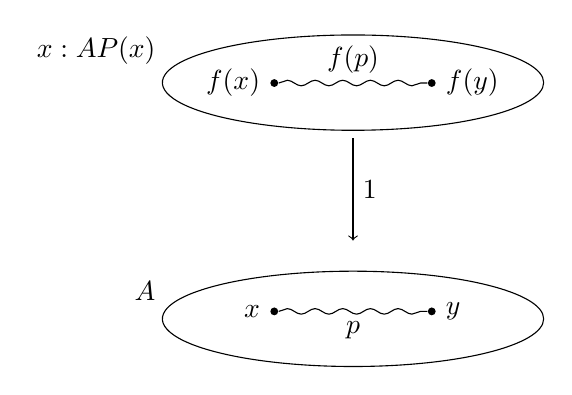
\begin{tikzpicture}[yscale=.5,xscale=2]
        \draw (0,0) arc (-90:170:8ex) node[anchor=south east] {$A$} arc (170:270:8ex);
        \draw (0,6) arc (-90:170:8ex) node[anchor=south east] {$\sm{x:A} P(x)$} arc (170:270:8ex);
        \draw[->] (0,5.8) -- node[auto] {$\proj1$} (0,3.2);
        \node[circle,fill,inner sep=1pt,label=left:{$x$}] (b1) at (-.5,1.4) {};
        \node[circle,fill,inner sep=1pt,label=right:{$y$}] (b2) at (.5,1.4) {};
        \draw[decorate,decoration={snake,amplitude=1}] (b1) -- node[auto,swap] {$p$} (b2);
        \node[circle,fill,inner sep=1pt,label=left:{$f(x)$}] (b1) at (-.5,7.2) {};
        \node[circle,fill,inner sep=1pt,label=right:{$f(y)$}] (b2) at (.5,7.2) {};
        \draw[decorate,decoration={snake,amplitude=1}] (b1) -- node[auto] {$f(p)$} (b2);
    \end{tikzpicture}
\end{center}

We \emph{can} obtain such a thing from \cref{lem:map}.
Given $f:\prd{x:A} P(x)$, we can define a non-dependent function $f':A\to \sm{x:A} P(x)$ by setting $f'(x)\defeq (x,f(x))$, and then consider $\ap{f'}{p} : f'(x) = f'(y)$.
Since $\proj1 \circ f' \jdeq \idfunc[A]$, by \cref{lem:ap-functor} we have $\ap{\proj1}{\ap{f'}{p}} = p$; thus $\ap{f'}{p}$ does ``lie over'' $p$ in this sense.
However, it is not obvious from the \emph{type} of $\ap{f'}{p}$ that it lies over any specific path in $A$ (in this case, $p$), which is sometimes important.

The solution is to use the transport lemma.
By \cref{thm:path-lifting} we have a canonical path $\mathsf{lift}(u,p)$ from $(x,u)$ to $(y,\trans p u)$ which lies over $p$.
Thus, any path from $u:P(x)$ to $v:P(y)$ lying over $p$ should factor through $\mathsf{lift}(u,p)$, essentially uniquely, by a path from $\trans p u$ to $v$ lying entirely in the fiber $P(y)$.
Thus, up to equivalence, it makes sense to define ``a path from $u$ to $v$ lying over $p:x=y$'' to mean a path $\trans p u = v$ in $P(y)$.
And, indeed, we can show that dependent functions produce such paths.

\begin{lem}[依值映射]
    \label{lem:mapdep}
    \indexdef{应用!依值函数到一个路径}%
    \indexdef{路径!依值函数的应用}%
    \indexdef{函数!依值!应用到路径}%
    \indexdef{动作!路径的依值函数的}%
    提供 $f:\prd{x: A} P(x)$; 然后有一个映射
    \[\apdfunc f : \prd{p:x=y}\big(\id[P(y)]{\trans p{f(x)}}{f(y)}\big).\]
\end{lem}

\begin{proof}[第一个证明]
    令 $D:\prd{x,y:A} (\id{x}{y}) \to \type$ 为一个如下定义的类型族
    \begin{equation*}
        D(x,y,p)\defeq \trans p {f(x)}= f(y).
    \end{equation*}
    然后 $D(x,x,\refl{x})$ 是 $\trans{(\refl{x})}{f(x)}= f(x)$.
    但是因为 $\trans{(\refl{x})}{f(x)}\jdeq f(x)$, 得到 $D(x,x,\refl{x})\jdeq (f(x)= f(x))$.
    因此, 有这个饿函数
    \begin{equation*}
        d\defeq\lam{x} \refl{f(x)}:\prd{x:A} D(x,x,\refl{x})
    \end{equation*}
    现在路径归纳给出对于每个 $p:x= y$ 有 $\apdfunc f(p):\trans p{f(x)}= f(y)$ .
\end{proof}

\begin{proof}[第二个证明]
    通过归纳, 可以假设 $p$ 是 $\refl x$.
    这个情况下, 所需的等式 $\trans{(\refl{x})}{f(x)}= f(x)$ 命题上成立.
\end{proof}

We will refer generally to paths which ``lie over other paths'' in this sense as \emph{dependent paths}.
\indexsee{dependent!path}{path, dependent}%
\index{path!dependent}%
They will play an increasingly important role starting in \cref{cha:hits}.
In \cref{sec:computational} we will see that for a few particular kinds of type families, there are equivalent ways to represent the notion of dependent paths that are sometimes more convenient.

现在回顾\cref{sec:pi-types}, 非依值类型函数 $f:A\to B$ 是依值函数 $f:\prd{x:A} P(x)$ 在 $P$ 是静态类型族 $P(x) \defeq B$ 的特殊情况.
这种情况下, $\apdfunc{f}$ 和 $\apfunc{f}$ 是密切相关的, 因为如下定理:

\begin{lem}
    \label{thm:trans-trivial}
    如果 $P:A\to\type$ 定义为 $P(x) \defeq B$ 对于固定的 $B:\type$, 那么对于任何 $x,y:A$ 和 $p:x=y$ 和 $b:B$ 有路径
    \[ \transconst Bpb : \transfib P p b = b. \]
\end{lem}
\begin{proof}[第一个证明]
    固定 $b:B$, 然后令 $D:\prd{x,y:A} (\id{x}{y}) \to \type$ 为一个类型族, 定义为
    \[ D(x,y,p) \defeq (\transfib P p b = b). \]
    然后 $D(x,x,\refl x)$ is $(\transfib P{\refl{x}}{b} = b)$, 通过运输的计算规则与 $(b=b)$ 判断等同.
    因此, 有这个函数
    \[ d \defeq \lam{x} \refl{b} : \prd{x:A} D(x,x,\refl x). \]
    现在路径归纳可以给出所需的元素
    \narrowequation{
        \prd{x,y:A}{p:x=y}(\transfib P p b = b).}
\end{proof}
\begin{proof}[第二个证明]
    通过归纳, 可以假设 $y$ 是 $x$ 而且 $p$ 是 $\refl x$.
    但是 $\transfib P {\refl x} b \jdeq b$, 所以这种情况下必须证明 $b=b$, 为此可以使用 $\refl{b}$.
\end{proof}

因此, 对于任何 $x,y:A$ 和 $p:x=y$ 和 $f:A\to B$, 通过分别连接 $\transconst Bp{f(x)}$ 和它的反转, 得到函数
\begin{align}
    \big(f(x) = f(y)\big) &\to \big(\trans{p}{f(x)} = f(y)\big)\label{eq:ap-to-apd}
    \qquad\text{和} \\
    \big(\trans{p}{f(x)} = f(y)\big) &\to \big(f(x) = f(y)\big).\label{eq:apd-to-ap}
\end{align}
事实上, 这些函数反向等价(它的意义会在\cref{sec:basics-equivalences}引入), 并且它们关联了 $\apfunc f (p)$ 和 $\apdfunc f (p)$.

\begin{lem}
    \label{thm:apd-const}
    对于 $f:A\to B$ 和 $p:\id[A]xy$, 有
    \[ \apdfunc f(p) = \transconst B p{f(x)} \ct \apfunc f (p). \]
\end{lem}
\begin{proof}[第一个证明]
    令 $D:\prd{x,y:A} (\id xy) \to \type$ 为类型族, 定义为
    \[ D(x,y,p) \defeq \big(\apdfunc f (p) = \transconst Bp{f(x)} \ct \apfunc f (p)\big). \]
    因此有
    \[D(x,x,\refl x) \jdeq \big(\apdfunc f (\refl x) = \transconst B{\refl x}{f(x)} \ct \apfunc f ({\refl x})\big).\]
    通过定义, 这个类型中出现的三个路径都是 $\refl{f(x)}$, 所以有
    \[ \refl{\refl{f(x)}} : D(x,x,\refl x). \]
    于是, 路径归纳给出所需的元素 $\prd{x,y:A}{p:x=y} D(x,y,p)$.
\end{proof}
\begin{proof}[第二个证明]
    通过归纳, 足以假定 $y$ 是 $x$ 而且 $p$ 是 $\refl x$.
    这个情况下, 需要证明的是 $\refl{f(x)} = \refl{f(x)} \ct \refl{f(x)}$, 判断上为真.
\end{proof}

因为 $\apdfunc{f}$ 和 $\apfunc{f}$ 的类型不同, 使用不同的符号会更清晰.
% We may sometimes use a notation $\apd f p$ for $\apdfunc{f}(p)$, which is similar to the notation $\ap f p$ for $\apfunc{f}(p)$.

\index{函数!依值|)}%

至此, 希望读者开始找到一些通过恒等类型的归纳做证明的感觉.
从现在开始不再给出两种风格的证明, 而是使用更清晰和使用的 (大部分情况是更简明的第二种).
这里有一些实用的运输定理; 留给读者做证明 (用两种风格).

\begin{lem}
    \label{thm:transport-concat}
    给定 $P:A\to\type$ 和 $p:\id[A]xy$ 与 $q:\id[A]yz$ 并且 $u:P(x)$, 有
    \[ \trans{q}{\trans{p}{u}} = \trans{(p\ct q)}{u}. \]
\end{lem}

\begin{lem}
    \label{thm:transport-compose}
    对于函数 $f:A\to B$ 和类型族 $P:B\to\type$, 和任意 $p:\id[A]xy$ 与 $u:P(f(x))$, 有
    \[ \transfib{P\circ f}{p}{u} = \transfib{P}{\apfunc f(p)}{u}. \]
\end{lem}

\begin{lem}
    \label{thm:ap-transport}
    对于 $P,Q:A\to \type$ 和函数的族 $f:\prd{x:A} P(x)\to Q(x)$, 和任意 $p:\id[A]xy$ 与 $u:P(x)$, 有
    \[ \transfib{Q}{p}{f_x(u)} = f_y(\transfib{P}{p}{u}). \]
\end{lem}

\index{type!family of|)}%
\index{transport|)}

\section{同伦和等价}
\label{sec:basics-equivalences}
\index{同伦|(defstyle}%

迄今为止, 已经见过了恒等类型 $\id[A]xy$ 可以被视为类型 $A$ 的两个元素 $x$ 与~$y$ 之间的 \emph{恒等}, \emph{路径}, 或者 \emph{等价}.
现在要研究一个合适的符号, 表示\emph{函数}和\emph{类型}之间的``恒等'' 或者 ``相同''.
在\cref{sec:compute-pi,sec:compute-universe}可以看到, 同伦类型论允许使用恒等类型的实例来标识它们, 不过在此之前需要清楚它们本身.

传统上, 两个函数相同就是对于所有输入, 它们得到相同的值.
按照命题作为类型的理解, 如果类型 $\prd{x:A} (f(x)=g(x))$ 有居留元, 这两个函数 $f$ 和 $g$ (也许是依值类型) 是相同的.
按照同伦论的理解, 这个依赖函数类型由\emph{连续的}路径或者\emph{函子}等价组成, 因此可以被视为\emph{同伦}的类型或者\emph{自然同构}.\index{同构!自然}
为此, 我们采用拓扑的术语.

\begin{defn}
    \label{defn:homotopy}
    令 $f,g:\prd{x:A} P(x)$ 为类型族 $P:A\to\type$ 的两个截面.
    从 $f$ 到 $g$ 的\define{同伦}是一个依赖函数, 它的类型为
    \begin{equation*}
    (f\htpy g)
        \defeq \prd{x:A} (f(x)=g(x)).
    \end{equation*}
\end{defn}

注意同伦并不是恒等 $(f=g)$.
不过, 在\cref{sec:compute-pi}会引入一个公理让同伦和恒等``等价''.

下面的证明留给读者.

\begin{lem}
    \label{lem:homotopy-props}
    在 $\prd{x:A} P(x)$ 的元素上, 同伦是它们各自的等价关系.
    也就是, 有这些类型的元素
    \begin{gather*}
        \prd{f:\prd{x:A} P(x)} (f\htpy f)\\
        \prd{f,g:\prd{x:A} P(x)} (f\htpy g) \to (g\htpy f)\\
        \prd{f,g,h:\prd{x:A} P(x)} (f\htpy g) \to (g\htpy h) \to (f\htpy h).
    \end{gather*}
\end{lem}

% This is judgmental and is \cref{ex:composition}.
% \begin{lem}
%   Composition is associative and unital up to homotopy.
%   That is:
%   \begin{enumerate}
%   \item If $f:A\to B$ then $f\circ \idfunc[A]\htpy f\htpy \idfunc[B]\circ f$.
%   \item If $f:A\to B, g:B\to C$ and $h:C\to D$ then $h\circ (g\circ f) \htpy (h\circ g)\circ f$.
%   \end{enumerate}
% \end{lem}

\index{类型论中函数的函子性@类型论中函数的``函子性''}%
\index{类型论中函数的连续性@类型论中函数的``连续性''}%
就像在类型伦中, 函数是自然而然的``函子'', 同伦是自然而然的
\index{同伦的自然性@同伦的``自然性''}%
``自然变换''.
这里只对非依赖函数 $f,g:A\to B$ 做了声明和证明; 在\cref{ex:dep-htpy-natural}要求读者推广它们到依值类型.

回顾 $f:A\to B$ 和 $p:\id[A]xy$, 可以把 $\apfunc{f} (p)$ 写作 $\ap f p$.

\begin{lem}
    \label{lem:htpy-natural}
    令 $H:f\htpy g$ 为函数  $f,g:A\to B$ 之间的一个同伦, 并让 $p:\id[A]xy$. 则有
    \begin{equation*}
        H(x)\ct\ap{g}{p}=\ap{f}{p}\ct H(y).
    \end{equation*}
    把它画成一个交换律的示意图:\index{示意图}
    \begin{align*}
        \xymatrix{
            f(x) \ar@{=}[r]^{\ap fp} \ar@{=}[d]_{H(x)} & f(y) \ar@{=}[d]^{H(y)} \\
            g(x) \ar@{=}[r]_{\ap gp} & g(y)
        }
    \end{align*}
\end{lem}
\begin{proof}
    通过归纳, 可以假定 $p$ 为 $\refl x$.
    将代入自反 $\apfunc{f}$ 和 $\apfunc g$ 计算, 得到
    \[ H(x) \ct \refl{g(x)} = \refl{f(x)} \ct H(x). \]
    两边都等于 $H(x)$.
\end{proof}

\begin{cor}\label{cor:hom-fg}
  令 $H : f \htpy \idfunc[A]$ 为一个同伦, 其中 $f : A \to A$. 那么对于任何 $x : A$ 有 \[ H(f(x)) = \ap f{H(x)}. \]
  % The above path will be denoted by $\com{H}{f}{x}$.
\end{cor}
\noindent
这里 $f(x)$ 表示一般的代入 $x$ 到 $f$, 而 $\ap f{H(x)}$ 代表 $\apfunc{f}(H(x))$.
\begin{proof}
    根据 $H$ 的自然性, 得到下面这个路径交换示意图:
    \begin{align*}
        \xymatrix@C=3pc{
            ffx \ar@{=}[r]^-{\ap f{Hx}} \ar@{=}[d]_{H(fx)} & fx \ar@{=}[d]^{Hx} \\
            fx \ar@{=}[r]_-{Hx} & x
        }
    \end{align*}
    也就是, $\ap f{H x} \ct H x = H(f x) \ct H x$.
    现在 whisker by $\opp{(H x)}$ 来消去 $H x$, 得到所需的
    \[ \ap f{H x}
    = \ap f{H x} \ct H x \ct \opp{(H x)}
    = H(f x) \ct H x \ct \opp{(H x)}
    = H(f x)
    \]
    (其中隐藏了路径的结合律).
\end{proof}

当然, 就像函数的函子性 (\cref{lem:ap-functor}), \cref{lem:htpy-natural}中的等同是一个满足它自己的一致性的路径, 诸如此类.

\index{同伦|)}%

\index{等价|(}%
接着讲类型, 按照传统观点, 函数 $f:A\to B$ 是一个\emph{同构}, 则有一个函数 $g:B\to A$, 并满足组合 $f\circ g$ 和 $g\circ f$ 都逐点等于恒等函数, 即 $f \circ g \htpy \idfunc[B]$ 和 $g\circ f \htpy \idfunc[A]$.
\indexsee{同伦!等价}{等价}%
按照同伦论的观点, 它可以被称为\emph{同伦等价}, 而在范畴论上, 它可以被称为\emph{ (高阶) 广群的等价}.
然而, 在 proof-relevant 的数学,
\index{数学!proof-relevant}%
相应的类型
\begin{equation}
  \sm{g:B\to A} \big((f \circ g \htpy \idfunc[B]) \times (g\circ f \htpy \idfunc[A])\big)\label{eq:qinvtype}
\end{equation}
表现并不好.
例如, 对于同一个函数 $f:A\to B$, 有一些~\eqref{eq:qinvtype}的居留元, 彼此不同.
(这和高阶范畴论中观察到的密切相关, 通常要考虑\emph{伴随}等价\index{伴随!等价}而不是简单的等价.)
因为这个原因, 所以把~\eqref{eq:qinvtype}按照这个历史准确的, 但是带有贬义的名字来代替.

\begin{defn}\label{defn:quasi-inverse}
  对于一个函数 $f:A\to B$, 它的 \define{quasi-inverse}
  \indexdef{quasi-inverse}%
  \indexsee{函数的!quasi-inverse}{quasi-inverse}%
  是一个三元对 $(g,\alpha,\beta)$,由一个函数 $g:B\to A$ , 同伦 $\alpha:f\circ g\htpy \idfunc[B]$ 与 $\beta:g\circ f\htpy \idfunc[A]$ 组成.
\end{defn}

\symlabel{qinv}
因此,~\eqref{eq:qinvtype}是\emph{$f$ 的 quasi-inverses 的类型}; 把它记作 $\qinv(f)$.

\begin{eg}\label{eg:idequiv}
  \index{identity!function}%
  \index{function!identity}%
  恒等函数 $\idfunc[A]:A\to A$ 有一个 quasi-inverse, 由 $\idfunc[A]$ 本身给定, 其中的同论被定义为 $\alpha(y) \defeq \refl{y}$ 和 $\beta(x) \defeq \refl{x}$.
\end{eg}

\begin{eg}\label{eg:concatequiv}
  对于任何 $p:\id[A]xy$ 和 $z:A$, 函数
  \begin{align*}
    (p\ct \blank)&:(\id[A]yz) \to (\id[A]xz) \qquad\text{和}\\
    (\blank \ct p)&:(\id[A]zx) \to (\id[A]zy)
  \end{align*}
  有 quasi-inverses, 由 $(\opp p \ct \blank)$ 和 $(\blank \ct \opp p)$ 分别给定; 参见 \cref{ex:equiv-concat}.
\end{eg}

\begin{eg}\label{thm:transportequiv}
  对于任何 $p:\id[A]xy$ 和 $P:A\to\type$, 函数
  \[\transfib{P}{p}{\blank}:P(x) \to P(y)\]
  有一个由 $\transfib{P}{\opp p}{\blank}$ 给定的  quasi-inverse ; 可以从 \narrowbreak \cref{thm:transport-concat} 推出.
\end{eg}

\symlabel{basics-isequiv}\symlabel{basics:iso}
通常, \emph{同构}
\index{同构!集合的}
(和熟悉的词语比如\emph{双射}, 和关联的符号 $A\cong B$)
\index{双射}
只用于类型 $A$ 和 $B$ ``像一个集合''的情况 (参见 \cref{sec:basics-sets}).
这种情况下, 类型~\eqref{eq:qinvtype}没有问题.
改进符号 $\isequiv (f)$, 作为\emph{等价}, 有以下性质:%
\begin{enumerate}
    \item 对于每个 $f:A\to B$ 有函数 $\qinv(f) \to \isequiv (f)$.\label{item:be1}
    \item 类似地, 对于每个 $f$ 有 $\isequiv (f) \to \qinv(f)$; 因此他们两个逻辑上相等(参见 \cref{sec:pat}).\label{item:be2}
    \item 对于每两个 $e_1,e_2:\isequiv(f)$ 有 $e_1=e_2$.\label{item:be3}
\end{enumerate}
在\cref{cha:equivalences} 会看到 $\isequiv(f)$ 有一些不同的定义满足这三个性质, 而它们都是等价的.
现在, 为了让读者确定它存在, 只介绍最简单的定义:
\begin{equation}\label{eq:isequiv-invertible}
  \isequiv(f) \;\defeq\;
  \Parens{\sm{g:B\to A} (f\circ g \htpy \idfunc[B])}
  \times
  \Parens{\sm{h:B\to A} (h\circ f \htpy \idfunc[A])}.
\end{equation}
现在可以这样从这个定义展示~\ref{item:be1}和~\ref{item:be2}.
函数 $\qinv(f) \to \isequiv (f)$ 很容易通过提取 $(g,\alpha,\beta)$ 为 $(g,\alpha,g,\beta)$ 定义.
另外一个方向, 给定 $(g,\alpha,h,\beta)$, 令 $\gamma$ 为同伦组合
\[ g \overset{\beta}{\htpy} h\circ f\circ g \overset{\alpha}{\htpy} h, \]
即 $\gamma(x) \defeq \opp{\beta(g(x))} \ct \ap{h}{\alpha(x)}$.
现在定义 $\beta':g\circ f\htpy \idfunc[A]$ 为 $\beta'(x) \defeq \gamma(f(x)) \ct \beta(x)$.
于是 $(g,\alpha,\beta'):\qinv(f)$.

这个定义的性质~\ref{item:be3}, 也不难证明, 不过需要笛卡尔积和依赖对子类型的声明恒等类型, 会在\cref{sec:compute-cartprod,sec:compute-sigma}中讨论.
因此降其推迟到\cref{sec:biinv}.
现在最重要的事是有了一个表现良好的类型来表示``$f$ 是一个等价'', 而且可以通过 quasi-inverse 来证明 $f$ 是一个等价.
实际上, 这是证明一个函数是一个等价的通用的方法.

和 proof-relevant 的哲学一致,
\index{数学!proof-relevant}%
从 $A$ 到 $B$ 的\emph{一个等价}定义为一个函数 $f:A\to B$ 与一个 $\isequiv (f)$ 的居留元, 即它们等价的一个证明.
将从 $A$ 到 $B$ 的等价的类型写作 $(\eqv A B)$, 即
\begin{equation}\label{eq:eqv}
  (\eqv A B) \defeq \sm{f:A\to B} \isequiv(f).
\end{equation}
之前的性质~\ref{item:be3} 确保了两个等价中的函数是相等的(也就是说, $A\to B$ 的元素之间相等), 那么等价也是相等的 (参见 \cref{sec:compute-sigma}).
因此, 经常滥用这个符号, 并模糊在等价和它的底层函数之间的区别.
如果有函数 $f:A\to B$ 并知道 $e:\isequiv(f)$, 可以写作 $f:\eqv A B$, 而不是 $\tup{f}{e}$.
反过来, 如果有一个等价 $g:\eqv A B$, 给定 $a:A$, 可以写作 $g(a)$, 而不是 $(\proj1 g)(a)$.

通过观察得出:

\begin{lem}
    \label{thm:equiv-eqrel}
    等价的类型是一个 \type 上的等价关系.
    更准确地说:
    \begin{enumerate}
        \item 对于任何 $A$, 恒等函数 $\idfunc[A]$ 是等价; 因此 $\eqv A A$.
        \item 对于任何 $f:\eqv A B$, 存在等价 $f^{-1} : \eqv B A$.
        \item 对于任何 $f:\eqv A B$ 和 $g:\eqv B C$, 存在 $g\circ f : \eqv A C$.
    \end{enumerate}
\end{lem}
\begin{proof}
  显然恒等函数是它自己的 quasi-inverse; 因此它是一个等价.

  如果 $f:A\to B$ 是等价, 那么它有 quasi-inverse, 叫做 $f^{-1}:B\to A$.
  然后 $f$ 也是 $f^{-1}$ 的 quasi-inverse, 所以 $f^{-1}$ 是等价 $B\to A$.

  最后, 给定 $f:\eqv A B$ 和 $g:\eqv B C$ 与 quasi-inverses $f^{-1}$ 和 $g^{-1}$, 然后对于任何 $a:A$ 有 $f^{-1} g^{-1} g f a = f^{-1} f a = a$, 对于任何 $c:C$ 有 $g f f^{-1} g^{-1} c = g g^{-1} c = c$.
  然后 $f^{-1} \circ g^{-1}$ 是 $g\circ f$ 的 quasi-inverse, 所以后者是一个等价.
\end{proof}

\index{等价|)}%

\section{类型的构造的高维群胚结构}
\label{sec:computational}
我们在 \cref{cha:typetheory}介绍了很多构造新类型的方式: 笛卡尔积, 不交并, 依值乘积, 依值和, 等等.
在 \cref{sec:equality,sec:functors,sec:fibrations}, 可以看到同伦类型论中\emph{所有}类型具备空间或者高维群胚的特征.
本章的目标是搞清楚 \cref{cha:typetheory} 中定义的特定类型的高维结构特征.

事实证明, 对于很多类型 $A$, 等同类型 $\id[A]xy$ 可以用构成 $A$ 的数据等价地表征.
例如, 如果 $A$ 是一个笛卡尔积 $B\times C$, 而 $x\jdeq (b,c)$ 和 $y\jdeq(b',c')$, 那么有等价
\begin{equation}\label{eq:prodeqv}
  \eqv{\big((b,c)=(b',c')\big)}{\big((b=b')\times (c=c')\big)}.
\end{equation}
更传统的语言中, 只有在两个有序对子的组成部分都相等时, 它们才相等(而等价~\eqref{eq:prodeqv} 有更多的含义).
这些等价关系的式子, 也能表达恒等类型的高阶结构;
例如, 连接两个序对间的等同相当于它的组成部分逐对地连接.

类似地, 类型族 $P:A\to\type$, 如果它由 \cref{cha:typetheory} 中的类型形成规则逐纤维地构造, 运算 $\transfib{P}{p}{\blank}$ 可以用进入 $P$ 的数据上对应的运算同伦地表征.
例如, 如果 $P(x) \jdeq B(x)\times C(x)$, 那么有
\[\transfib{P}{p}{(b,c)} = \big(\transfib{B}{p}{b},\transfib{C}{p}{c}\big).\]

最后, 类型形成规则也是函子性的, 如果用这些函子构造函数 $f$, 那么可以基于进入 $f$ 的数据, 得到运算 $\apfunc f$ 和 $\apdfunc f$.
例如, 如果 $g:B\to B'$ 和 $h:C\to C'$ 并将 $f:B\times C \to B'\times C'$ 定义为 $f(b,c)\defeq (g(b),h(c))$, 然后根据等价~\eqref{eq:prodeqv}, 可以将 $\apfunc f$ 表示为 ``$(\apfunc g,\apfunc h)$''.

接下来的小节 (\crefrange{sec:compute-cartprod}{sec:compute-nat}) 会专注于陈述和证明那些基础类型的形成规则, 每个小节对应一个基础类型形成器.
目前的类型论中, 明显地缺乏某些东西;
接下来的章节中, 恒等类型, 运输等\emph{判断}\index{判断等同}等同, 可以更方便和直观地描述.
然而, \cref{cha:typetheory} 提出的理论中, 恒等类型被其归纳原理对于所有类型统一定义, 所以无法 ``重新定义'' 它们, 让它在不同类型下成为不同的东西.
因此, 本章讨论的哪些特定类型大部分是, 可以发现和证明的\emph{定理}.

实际上, \cref{cha:typetheory}的类型论不足以证明这两个类型的形成器: $\Pi$-类型和全集.
因此, 我们被迫引入公理到我们的类型论中, 来让这些``定理''为真.
类型论上, 一个\emph{公理} (比较~\cref{sec:axioms}) 是一个``原子性''元素, 它被声明是特定类型的居留元, 没有任何规则管理它的行为, 除了这些它的居留类型.
\index{公理!与规则}%

\index{函数外延性}%
\indexsee{外延性, 函数的}{函数外延性}
\index{一价公理}%
$\Pi$-类型的公理(\cref{sec:compute-pi}) 是类型论学家熟悉的: \emph{函数外延性}, 粗略地说就是, 若两个函数在 \cref{sec:basics-equivalences} 的意义上是同伦的, 那么它们相等.
而全集的公理 (\cref{sec:compute-universe}), 是 Voevodsky 对同伦类型论的新贡献: 被称为\emph{一价公理}, 粗略地说就是, 若两个类型等价(\cref{sec:basics-equivalences}), 那么它们相等.
在导论中已经见过这个公理; 这本书中它将扮演一个重要角色.%
\footnote{我们选择引入这些原则作为公理, 但还有潜在地其它方法, 来指定一个它们成立的类型论.
  参见本章的备注.}

值得注意的是, 不是\emph{所有}恒等类型可以通过在类型的构造上归纳来``确定''.
反例包含了大部分非平凡高维归纳类型 (参见 \cref{cha:hits,cha:homotopy}).
例如, 计算类型 $\Sn^n$ 的恒等类型 (参见 \cref{sec:circle}) 等价于球的计算高维同伦群, 代数拓扑学的一个深刻而重要的研究领域.

\section{笛卡尔积类型}
\label{sec:compute-cartprod}
\index{类型!积|(}%
给定类型 $A$ 和 $B$, 考虑笛卡尔积类型 $A \times B$.
对于任何元素 $x,y:A\times B$ 和路径 $p:\id[A\times B]{x}{y}$, 根据函子性可以提取类型 $\ap{\proj1}p:\id[A]{\proj1(x)}{\proj1(y)}$ 和 $\ap{\proj2}p:\id[B]{\proj2(x)}{\proj2(y)}$.
因此有函数
\begin{equation}
    \label{eq:path-prod}
    (\id[A\times B]{x}{y}) \to (\id[A]{\proj1(x)}{\proj1(y)}) \times (\id[B]{\proj2(x)}{\proj2(y)}).
\end{equation}

\begin{thm}
    \label{thm:path-prod}
    对于任何 $x$ 和 $y$, 函数~\eqref{eq:path-prod} 是一个等价.
\end{thm}

从逻辑上阅读, 这说明两个对子相等, 就是它逐组成地相等.
从范畴论上看, 这说明积群胚中的态射是态射的对子.
从同伦论上看, 这说明积空间中的路径是路径的对子.

\begin{proof}
    需要另一个方向的函数:
    \begin{equation}
    (\id[A]{\proj1(x)}{\proj1(y)})
        \times (\id[B]{\proj2(x)}{\proj2(y)}) \to (\id[A\times B]{x}{y}). \label{eq:path-prod-inverse}
    \end{equation}
    根据笛卡尔积的归纳规则, 可以任务 $x$ 和 $y$ 都是对子, 也就是 $x\jdeq (a,b)$ 和 $y\jdeq (a',b')$ 其中 $a,a':A$ 而 $b,b':B$.
    这种情况下, 想要的就是函数
    \begin{equation*}
    (\id[A]{a}{a'})
        \times (\id[B]{b}{b'}) \to \big(\id[A\times B]{(a,b)}{(a',b')}\big).
    \end{equation*}
    现在, 在它的定义域进行笛卡尔积的归纳, 可以认为 $p:a=a'$ 和 $q:b=b'$.
    经过两次路径归纳, 可以认为 $a\jdeq a'$ 和 $b\jdeq b'$ 而 $p$ 和 $q$ 都为自反.
    这种个情况下, 有 $(a,b)\jdeq(a',b')$, 所以可以用自反作为输出.

    接下来证明~\eqref{eq:path-prod-inverse} 准逆于 ~\eqref{eq:path-prod}.
    只需简单连续使用递归, 不过必须按照正确的顺序来.

    其中一个方向, 从 $r:\id[A\times B]{x}{y}$ 开始.
    首先在 $r$ 上进行路径归纳, 并认为 $x\jdeq y$ 而且 $r$ 是自反.
    这种情况下, 因为 $\apfunc{\proj1}$ 和 $\apfunc{\proj2}$ 是通过路径归纳定义的,~\eqref{eq:path-prod} 将 $r\jdeq \refl{x}$ 变为序对 $(\refl{\proj1x},\refl{\proj2x})$.
    对 $x$ 归纳, 可以假定 $x\jdeq (a,b)$, 于是它就是 $(\refl a, \refl b)$.
    因此, 根据定义, ~\eqref{eq:path-prod-inverse} 得到 $\refl{(a,b)}$, 即 (根据目前的假定) $r$.

    另一个方向, 如果从 $s:(\id[A]{\proj1(x)}{\proj1(y)}) \times (\id[B]{\proj2(x)}{\proj2(y)})$ 开始, 首先对 $x$ 和 $y$ 归纳, 假定它们分别是对子 $(a,b)$ 和 $(a',b')$, 然后对 $s:(\id[A]{a}{a'}) \times (\id[B]{b}{b'})$ 归纳来化简到对子 $(p,q)$, 其中 $p:a=a'$ 而 $q:b=b'$.
    现在对 $p$ 和 $q$ 归纳, 假定它们是自反 $\refl a$ 和 $\refl b$, 这种情况~\eqref{eq:path-prod-inverse} 得到 $\refl{(a,b)}$ 而~\eqref{eq:path-prod} 返回 $(\refl a,\refl b)\jdeq (p,q)\jdeq s$.
\end{proof}

特别地, 我们展示了~\eqref{eq:path-prod} 有一个逆~\eqref{eq:path-prod-inverse}, 可以记作
\symlabel{defn:pairpath}
\[
    \pairpath : (\id{\proj{1}(x)}{\proj{1}(y)}) \times (\id{\proj{2}(x)}{\proj{2}(y)}) \to (\id x y).
\]
注意这个特殊情况, 得到了乘积类型命题上的唯一性原理\index{唯一性!原理, 命题!乘积类型的}: $z = (\proj1(z),\proj2(z))$.

可以将 \pairpath 看作 $\id x y$ 的\emph{构造器}或者\emph{构造规则}, 类似于 $A\times B$ 自己的``对子''构造器, 即给定 $a:A$ 和 $b:B$ 构造对子 $(a,b)$.
从这个观点, ~\eqref{eq:path-prod} 的两个组成部分:
\begin{align*}
    \projpath{1} &: (\id{x}{y}) \to (\id{\proj{1}(x)}{\proj{1} (y)})\\
    \projpath{2} &: (\id{x}{y}) \to (\id{\proj{2}(x)}{\proj{2} (y)})
\end{align*}
是\emph{消去}规则.
类似的, 这两个同伦, 也就是 ~\eqref{eq:path-prod-inverse} 准逆于 ~\eqref{eq:path-prod} 的证据, 分别是\emph{命题上的计算规则}:
\index{计算规则!命题上的!对子间的恒等}%
\begin{align*}
{\projpath{1}{(\pairpath(p, q)})}
    &= %_{(\id{\proj{1} x}{\proj{1} y})}
        {p} \\
    {\projpath{2}{(\pairpath(p,q)})}
    &= %_{(\id{\proj{2} x}{\proj{2} y})}
        {q}
\end{align*}
对于 $p:\id{\proj{1} x}{\proj{1} y}$ 和 $q:\id{\proj{2} x}{\proj{2} y}$, 有一个\emph{命题上的唯一性原理}:
\index{唯一性!原理, 命题上的!对于对子之间的恒等}%
\[
    \id{r}{\pairpath(\projpath{1} (r), \projpath{2} (r)) }
    \qquad\text{for } r : \id[A \times B] x y.
\]

对于 $A\times B$ 每个组件的路径, 可以表征自反, 逆, 和组合:
\begin{align*}
{\refl{(z : A \times B)}}
    &= {\pairpath (\refl{\proj{1} z},\refl{\proj{2} z})} \\
    {\opp{p}}
    &= {\pairpath \big(\opp{\projpath{1} (p)},\, \opp{\projpath{2} (p)}\big)} \\
    {{p \ct q}}
    &= {\pairpath \big({\projpath{1} (p)} \ct {\projpath{1} (q)},\,{\projpath{2} (p)} \ct {\projpath{2} (q)}\big)}.
\end{align*}
或者, 写作:
\begin{alignat*}{2}
    \projpath{i}(\refl{(z : A \times B)}) &= \refl{\proj{i} z} &\qquad (i=1,2)\\
    \pairpath(\opp p, \opp q) &= \opp{\pairpath(p,q)}\\
    \pairpath(p\ct q, p'\ct q') &= \pairpath(p,p') \ct \pairpath(q,q').
\end{alignat*}
这些等式全都可以这样推导出来, 通过对给定的路径进行路径归纳, 然后返回自反.
\cref{sec:equality} 中高维群胚结构的剩余部分也同样符合, 尽管这会变得冗长, 要插入足够多的其它连贯路径, 来得到一个通过类型检查的等式.
例如, 如果要表示 \cref{thm:omg}\ref{item:omg4} 中路径的逆, 其中使用 $\ctassoc(p,q,r)$ 并用 $\pairct(p,q,p',q')$ 表示上面的最后一个路径, 然后对于任何 $u,v,z,w:A\times B$ 和 $p,q,r,p',q',r'$ 属于合适的类型, 有
\begin{equation*}
    \begin{array}{l}
        \pairct(p\ct q, r, p'\ct q', r')                                    \\
        \ct\;  (\pairct(p,q,p',q') \rightwhisker \pairpath(r,r'))             \\
        \ct\;  \ctassoc(\pairpath(p,p'),\pairpath(q,q'),\pairpath(r,r'))      \\
        =
        \begin{array}[t]{l}
            \apfunc{\pairpath}({\pairpath(\ctassoc(p,q,r),\ctassoc(p',q',r'))}) \\
            \ct\; \pairct(p, q\ct r, p', q'\ct r')                              \\
            \ct\; (\pairpath(p,p') \leftwhisker \pairct(q,r,q',r')).
        \end{array}
    \end{array}
\end{equation*}
幸运的是, 之后将不会使用任何这样的高维连贯.

\index{运输!乘积类型中}%
现在考虑在类型族逐点的乘积中的运输.
给定类型族 $ A, B : Z \to \type$, 滥用地写作 $A\times B:Z\to \type$ 对于定义为 $(A\times B)(z) \defeq A(z) \times B(z)$ 的类型族.
现在给定 $p : \id[Z]{z}{w}$ 和 $x : A(z) \times B(z)$, 可以沿着 $p$ 运输 $x$ 得到一个 $A(w)\times B(w)$ 元素.

\begin{thm}
    \label{thm:trans-prod}
    上述情况下, 有
    \[
        \id[A(w) \times B(w)]
            {\transfib{A\times B}px}
            {(\transfib{A}{p}{\proj{1}x}, \transfib{B}{p}{\proj{2}x})}.
    \]
\end{thm}
\begin{proof}
    根据路径归纳, 可以假定 $p$ 是自反, 其中
    \begin{align*}
        \transfib{A\times B}px&\jdeq x\\
        \transfib{A}{p}{\proj{1}x}&\jdeq \proj1x\\
        \transfib{B}{p}{\proj{2}x}&\jdeq \proj2x.
    \end{align*}
    因此, 还要展示 $x = (\proj1 x, \proj2x)$.
    而这就是乘积类型命题的唯一性公理, 之前备注过, 来自 \cref{thm:path-prod}.
\end{proof}

最后, 考虑笛卡尔积上的 $\apfunc{}$ 的函子性.
给定类型 $A,B,A',B'$ 与函数 $g:A\to A'$ 和 $h:B\to B'$;
然后可以定义函数 $f:A\times B\to A'\times B'$ 通过 $f(x) \defeq (g(\proj1x),h(\proj2x))$.

\begin{thm}
    \label{thm:ap-prod}
    上述情况下, 给定 $x,y:A\times B$ 和 $p:\proj1x=\proj1y$ 以及 $q:\proj2x=\proj2y$, 有
    \[ \id[(f(x)=f(y))]{\ap{f}{\pairpath(p,q)}} {\pairpath(\ap{g}{p},\ap{h}{q})}. \]
\end{thm}
\begin{proof}
    注意, 首先上面的等式是良类型的.
    一方面, 因为 $\pairpath(p,q):x=y$ 有 $\ap{f}{\pairpath(p,q)}:f(x)=f(y)$.
    另一方面, 因为 $\proj1(f(x))\jdeq g(\proj1x)$ 和 $\proj2(f(x))\jdeq h(\proj2x)$, 同样有 $\pairpath(\ap{g}{p},\ap{h}{q}):f(x)=f(y)$.

    现在, 通过归纳, 可以假定 $x\jdeq(a,b)$ 和 $y\jdeq(a',b')$, 这种情况下有 $p:a=a'$ 和 $q:b=b'$.
    因此, 通过路径归纳, 可以假定 $p$ 和 $q$ 是自反的, 这种情况下所需的等式判断地成立.
\end{proof}

\index{类型!乘积|)}%

\section{\texorpdfstring{$\Sigma$}{Σ}-类型}
\label{sec:compute-sigma}
\index{type!dependent pair|(}%
Let $A$ be a type and $P:A\to\type$ a type family.
Recall that the $\Sigma$-type, or dependent pair type, $\sm{x:A} P(x)$ is a generalization of the cartesian product type.
Thus, we expect its higher groupoid structure to also be a generalization of the previous section.
In particular, its paths should be pairs of paths, but it takes a little thought to give the correct types of these paths.

Suppose that we have a path $p:w=w'$ in $\sm{x:A}P(x)$.
Then we get $\ap{\proj{1}}{p}:\proj{1}(w)=\proj{1}(w')$.
However, we cannot directly ask whether $\proj{2}(w)$ is identical to $\proj{2}(w')$ since they don't have to be in the same type.
But we can transport\index{transport} $\proj{2}(w)$ along the path $\ap{\proj{1}}{p}$, and this does give us an element of the same type as $\proj{2}(w')$.
By path induction, we do in fact obtain a path $\trans{\ap{\proj{1}}{p}}{\proj{2}(w)}=\proj{2}(w')$.

Recall from the discussion preceding \cref{lem:mapdep} that
\narrowequation{
  \trans{\ap{\proj{1}}{p}}{\proj{2}(w)}=\proj{2}(w')
}
can be regarded as the type of paths from $\proj2(w)$ to $\proj2(w')$ which lie over the path $\ap{\proj1}{p}$ in $A$.
\index{fibration}%
\index{total!space}%
Thus, we are saying that a path $w=w'$ in the total space determines (and is determined by) a path $p:\proj1(w)=\proj1(w')$ in $A$ together with a path from $\proj2(w)$ to $\proj2(w')$ lying over $p$, which seems sensible.

\begin{rmk}
  Note that if we have $x:A$ and $u,v:P(x)$ such that $(x,u)=(x,v)$, it does not follow that $u=v$.
  All we can conclude is that there exists $p:x=x$ such that $\trans p u = v$.
  This is a well-known source of confusion for newcomers to type theory, but it makes sense from a topological viewpoint: the existence of a path $(x,u)=(x,v)$ in the total space of a fibration between two points that happen to lie in the same fiber does not imply the existence of a path $u=v$ lying entirely \emph{within} that fiber.
\end{rmk}

The next theorem states that we can also reverse this process.
Since it is a direct generalization of \cref{thm:path-prod}, we will be more concise.

\begin{thm}\label{thm:path-sigma}
Suppose that $P:A\to\type$ is a type family over a type $A$ and let $w,w':\sm{x:A}P(x)$. Then there is an equivalence
\begin{equation*}
\eqvspaced{(w=w')}{\dsm{p:\proj{1}(w)=\proj{1}(w')} \trans{p}{\proj{2}(w)}=\proj{2}(w')}.
\end{equation*}
\end{thm}

\begin{proof}
We define a function
\begin{equation*}
f : \prd{w,w':\sm{x:A}P(x)} (w=w') \to \dsm{p:\proj{1}(w)=\proj{1}(w')} \trans{p}{\proj{2}(w)}=\proj{2}(w')
\end{equation*}
by path induction, with
\begin{equation*}
f(w,w,\refl{w})\defeq(\refl{\proj{1}(w)},\refl{\proj{2}(w)}).
\end{equation*}
We want to show that $f$ is an equivalence.

In the reverse direction, we define
\begin{narrowmultline*}
  g : \prd{w,w':\sm{x:A}P(x)}
      \Parens{\sm{p:\proj{1}(w)=\proj{1}(w')}\trans{p}{\proj{2}(w)}=\proj{2}(w')}
      \to
      \narrowbreak
      (w=w')
\end{narrowmultline*}
by first inducting on $w$ and $w'$, which splits them into $(w_1,w_2)$ and
$(w_1',w_2')$ respectively, so it suffices to show
\begin{equation*}
\Parens{\sm{p:w_1 = w_1'}\trans{p}{w_2}=w_2'} \to ((w_1,w_2)=(w_1',w_2')).
\end{equation*}
Next, given a pair $\sm{p:w_1 = w_1'}\trans{p}{w_2}=w_2'$, we can
use $\Sigma$-induction to get $p : w_1 = w_1'$ and $q :
\trans{p}{w_2}=w_2'$.  Inducting on $p$, we have $q :
\trans{(\refl{w_1})}{w_2}=w_2'$, and it suffices to show
$(w_1,w_2)=(w_1,w_2')$.  But $\trans{(\refl{w_1})}{w_2} \jdeq w_2$, so
inducting on $q$ reduces the goal to
$(w_1,w_2)=(w_1,w_2)$, which we can prove with $\refl{(w_1,w_2)}$.

Next we show that $f(g(r))=r$ for all $w$, $w'$ and
$r$, where $r$ has type
\[\dsm{p:\proj{1}(w)=\proj{1}(w')} (\trans{p}{\proj{2}(w)}=\proj{2}(w')).\]
First, we break apart the pairs $w$, $w'$, and $r$ by pair induction, as in the
definition of $g$, and then use two path inductions to reduce both components
of $r$ to \refl{}.  Then it suffices to show that
$f (g(\refl{w_1},\refl{w_2})) = (\refl{w_1},\refl{w_2})$, which is true by definition.

Similarly, to show that $g(f(p))=p$ for all $w$, $w'$,
and $p : w = w'$, we can do path induction on $p$, and then pair induction to
split $w$, at which point it suffices to show that
$g(f (\refl{(w_1,w_2)})) = \refl{(w_1,w_2)}$, which is true by
definition.

Thus, $f$ has a quasi-inverse, and is therefore an equivalence.
\end{proof}

As we did in the case of cartesian products, we can deduce a propositional uniqueness principle as a special case.

\begin{cor}\label{thm:eta-sigma}
  \index{uniqueness!principle, propositional!for dependent pair types}%
  For $z:\sm{x:A} P(x)$, we have $z = (\proj1(z),\proj2(z))$.
\end{cor}
\begin{proof}
  We have $\refl{\proj1(z)} : \proj1(z) = \proj1(\proj1(z),\proj2(z))$, so by \cref{thm:path-sigma} it will suffice to exhibit a path $\trans{(\refl{\proj1(z)})}{\proj2(z)} = \proj2(\proj1(z),\proj2(z))$.
  But both sides are judgmentally equal to $\proj2(z)$.
\end{proof}

Like with binary cartesian products, we can think of
the backward direction of \cref{thm:path-sigma} as
an introduction form (\pairpath{}{}), the forward direction as
elimination forms (\projpath{1} and \projpath{2}), and the equivalence
as giving a propositional computation rule and uniqueness principle for these.

Note that the lifted path $\mathsf{lift}(u,p)$  of $p:x=y$ at $u:P(x)$ defined in \cref{thm:path-lifting} may be identified with the special case of the introduction form
\[\pairpath(p,\refl{\trans p u}):(x,u) = (y,\trans p u).\]
\index{transport!in dependent pair types}%
This appears in the statement of action of transport on $\Sigma$-types, which is also a generalization of the action for binary cartesian products:

\begin{thm}\label{transport-Sigma}
  Suppose we have type families
  %
  \begin{equation*}
    P:A\to\type
    \qquad\text{and}\qquad
    Q:\Parens{\sm{x:A} P(x)}\to\type.
  \end{equation*}
  %
  Then we can construct the type family over $A$ defined by
  \begin{equation*}
    x \mapsto \sm{u:P(x)} Q(x,u).
  \end{equation*}
  For any path $p:x=y$ and any $(u,z):\sm{u:P(x)} Q(x,u)$ we have
  \begin{equation*}
    \trans{p}{u,z}=\big(\trans{p}{u},\,\trans{\pairpath(p,\refl{\trans pu})}{z}\big).
  \end{equation*}
\end{thm}

\begin{proof}
Immediate by path induction.
\end{proof}

We leave it to the reader to state and prove a generalization of
\cref{thm:ap-prod} (see \cref{ex:ap-sigma}), and to characterize
the reflexivity, inverses, and composition of $\Sigma$-types
componentwise.

\index{type!dependent pair|)}%

\section{单元类型}
\label{sec:compute-unit}
\index{type!unit|(}%
有时平凡的事情也很重要, 所以简单提一下单元类型~\unit.

\begin{thm}\label{thm:path-unit}
  对于任何 $x,y:\unit$, 有 $\eqv{(x=y)}{\unit}$.
\end{thm}

也许会从 $x$ 和 $y$ 上的 $\unit$-归纳开始证明, 化简问题为 $\eqv{(\ttt=\ttt)}{\unit}$.
然而, 会卡住在这个点上, 无法在 $p:\ttt=\ttt$ 上作路径归纳.
因此, 改为尽可能地使用通用的 $x$ 和 $y$, 最后才用归纳化简它们到 $\ttt$.

\begin{proof}
  函数 $(x=y)\to\unit$ 很容易定义, 对于任何输入都返回 \ttt.
  反过来, 对于任何 $x,y:\unit$ 可以通过归纳假定 $x\jdeq \ttt\jdeq y$.
  这种情况下有 $\refl{\ttt}:x=y$, 得到常量函数 $\unit\to(x=y)$.

  为了展示它们互逆, 首先考虑元素 $u:\unit$.
  可以假定 $u\jdeq\ttt$, 而它也是这个组合 $\unit \to (x=y)\to\unit$ 的结果.

  另一变, 给定 $p:x=y$.
  通过路径归纳, 假定 $x\jdeq y$ 和 $p$ 是 $\refl x$.
  然后假定 $x$ 是 \ttt, 这种情况下, 组合 $(x=y) \to \unit\to(x=y)$ 传入 $p$ 返回 $\refl x$, 即~$p$.
\end{proof}

特别地, 任何两个 $\unit$ 的元素是相等的.
留给读者用表达式来形式该等价的构造, 消去, 计算, 和唯一性规则.
\index{传输!单元类型}%
\unit 的传输引理就是常量类型族的传输引理 (\cref{thm:trans-trivial}).

\index{类型!单元|)}%

\section{\texorpdfstring{$\Pi$}{Π}-types and the function extensionality axiom}
\label{sec:compute-pi}
\index{type!dependent function|(}%
\index{type!function|(}%
\index{homotopy|(}%
Given a type $A$ and a type family $B : A \to \type$, consider the dependent function type $\prd{x:A}B(x)$.
We expect the type $f=g$ of paths from $f$ to $g$ in $\prd{x:A} B(x)$ to be equivalent to
the type of pointwise paths:\index{pointwise!equality of functions}
\begin{equation}
  \eqvspaced{(\id{f}{g})}{\Parens{\prd{x:A} (\id[B(x)]{f(x)}{g(x)})}}.\label{eq:path-forall}
\end{equation}
From a traditional perspective, this would say that two functions which are equal at each point are equal as functions.
\index{continuity of functions in type theory@``continuity'' of functions in type theory}%
From a topological perspective, it would say that a path in a function space is the same as a continuous homotopy.
\index{functoriality of functions in type theory@``functoriality'' of functions in type theory}%
And from a categorical perspective, it would say that an isomorphism in a functor category is a natural family of isomorphisms.

Unlike the case in the previous sections, however, the basic type theory presented in \cref{cha:typetheory} is insufficient to prove~\eqref{eq:path-forall}.
All we can say is that there is a certain function
\begin{equation}\label{eq:happly}
  \happly : (\id{f}{g}) \to \prd{x:A} (\id[B(x)]{f(x)}{g(x)})
\end{equation}
which is easily defined by path induction.
For the moment, therefore, we will assume:

\begin{axiom}[Function extensionality]\label{axiom:funext}
  \indexsee{axiom!function extensionality}{function extensionality}%
  \indexdef{function extensionality}%
  For any $A$, $B$, $f$, and $g$, the function~\eqref{eq:happly} is an equivalence.
\end{axiom}

We will see in later chapters that this axiom follows both from univalence (see \cref{sec:compute-universe,sec:univalence-implies-funext}) and from an interval type (see \cref{sec:interval} and \cref{ex:funext-from-interval}).

In particular, \cref{axiom:funext} implies that~\eqref{eq:happly} has a quasi-inverse
\[
\funext : \Parens{\prd{x:A} (\id{f(x)}{g(x)})} \to {(\id{f}{g})}.
\]
This function is also referred to as ``function extensionality''.
As we did with $\pairpath$ in \cref{sec:compute-cartprod}, we can regard $\funext$ as an \emph{introduction rule} for the type $\id f g$.
From this point of view, $\happly$ is the \emph{elimination rule}, while the homotopies witnessing $\funext$ as quasi-inverse to $\happly$ become a propositional computation rule\index{computation rule!propositional!for identities between functions}
\[
\id{\happly({\funext{(h)}},x)}{h(x)} \qquad\text{for }h:\prd{x:A} (\id{f(x)}{g(x)})
\]
and a propositional uniqueness principle\index{uniqueness!principle!for identities between functions}:
\[
\id{p}{\funext (x \mapsto \happly(p,{x}))} \qquad\text{for } p: \id f g.
\]

We can also compute the identity, inverses, and composition in $\Pi$-types; they are simply given by pointwise operations:\index{pointwise!operations on functions}.
\begin{align*}
\refl{f} &= \funext(x \mapsto \refl{f(x)}) \\
\opp{\alpha} &= \funext (x \mapsto \opp{\happly (\alpha,x)})  \\
{\alpha} \ct \beta &= \funext (x \mapsto {\happly({\alpha},x) \ct \happly({\beta},x)}).
\end{align*}
The first of these equalities follows from the definition of $\happly$, while the second and third are easy path inductions.

Since the non-dependent function type $A\to B$ is a special case of the dependent function type $\prd{x:A} B(x)$ when $B$ is independent of $x$, everything we have said above applies in non-dependent cases as well.
\index{transport!in function types}%
The rules for transport, however, are somewhat simpler in the non-dependent case.
Given a type $X$, a path $p:\id[X]{x_1}{x_2}$, type families $A,B:X\to \type$, and a function $f : A(x_1) \to B(x_1)$,  we have
\begin{align}\label{eq:transport-arrow}
  \transfib{A\to B}{p}{f} &=
  \Big(x \mapsto \transfib{B}{p}{f(\transfib{A}{\opp p}{x})}\Big)
\end{align}
where $A\to B$ denotes abusively the type family $X\to \type$ defined by
\[(A\to B)(x) \defeq (A(x)\to B(x)).\]
In other words, when we transport a function $f:A(x_1)\to B(x_1)$ along a path $p:x_1=x_2$, we obtain the function $A(x_2)\to B(x_2)$ which transports its argument backwards along $p$ (in the type family $A$), applies $f$, and then transports the result forwards along $p$ (in the type family $B$).
This can be proven easily by path induction.

\index{transport!in dependent function types}%
Transporting dependent functions is similar, but more complicated.
Suppose given $X$ and $p$ as before, type families $A:X\to \type$ and $B:\prd{x:X} (A(x)\to\type)$, and also a dependent function $f : \prd{a:A(x_1)} B(x_1,a)$.
Then for $a:A(x_2)$, we have
\begin{narrowmultline*}
  \transfib{\Pi_A(B)}{p}{f}(a) = \narrowbreak
  \Transfib{\widehat{B}}{\opp{(\pairpath(\opp{p},\refl{ \trans{\opp p}{a} }))}}{f(\transfib{A}{\opp p}{a})}
\end{narrowmultline*}
where $\Pi_A(B)$ and $\widehat{B}$ denote respectively the type families
\begin{equation}\label{eq:transport-arrow-families}
\begin{array}{rclcl}
\Pi_A(B) &\defeq& \big(x\mapsto \prd{a:A(x)} B(x,a) \big) &:& X\to \type\\
\widehat{B} &\defeq& \big(w \mapsto B(\proj1w,\proj2w) \big) &:& \big(\sm{x:X} A(x)\big) \to \type.
\end{array}
\end{equation}
If these formulas look a bit intimidating, don't worry about the details.
The basic idea is just the same as for the non-dependent function type: we transport the argument backwards, apply the function, and then transport the result forwards again.

Now recall that for a general type family $P:X\to\type$, in \cref{sec:functors} we defined the type of \emph{dependent paths} over $p:\id[X]xy$ from $u:P(x)$ to $v:P(y)$ to be $\id[P(y)]{\trans{p}{u}}{v}$.
When $P$ is a family of function types, there is an equivalent way to represent this which is often more convenient.
\index{path!dependent!in function types}

\begin{lem}\label{thm:dpath-arrow}
  Given type families $A,B:X\to\type$ and $p:\id[X]xy$, and also $f:A(x)\to B(x)$ and $g:A(y)\to B(y)$, we have an equivalence
  \[ \eqvspaced{ \big(\trans{p}{f} = {g}\big) } { \prd{a:A(x)}  (\trans{p}{f(a)} = g(\trans{p}{a})) }. \]
  Moreover, if $q:\trans{p}{f} = {g}$ corresponds under this equivalence to $\widehat q$, then for $a:A(x)$, the path
  \[ \happly(q,\trans p a) : (\trans p f)(\trans p a) = g(\trans p a)\]
  is equal to the concatenated path $i\ct j\ct k$, where
  \begin{itemize}
  \item $i:(\trans p f)(\trans p a) = \trans p {f (\trans {\opp p}{\trans p a})}$ comes from~\eqref{eq:transport-arrow},
  \item $j:\trans p {f (\trans {\opp p}{\trans p a})} = \trans p {f(a)}$ comes from \cref{thm:transport-concat,thm:omg}, and
  \item $k:\trans p {f(a)}= g(\trans p a)$ is $\widehat{q}(a)$.
  \end{itemize}
\end{lem}
\begin{proof}
  By path induction, we may assume $p$ is reflexivity, in which case the desired equivalence reduces to function extensionality.
  The second statement then follows by the computation rule for function extensionality.
\end{proof}

In general, it happens quite frequently that we want to consider a concatenation of paths each of which arises from some previously proven lemmas or hypothesized objects, and it can be rather tedious to describe this by giving a name to each path in the concatenation as we did in the second statement above.
Thus, we adopt a convention of writing such concatenations in the familiar mathematical style of ``chains of equalities with reasons'', and allow ourselves to omit reasons that the reader can easily fill in.
For instance, the path $i\ct j\ct k$ from \cref{thm:dpath-arrow} would be written like this:
  \begin{align*}
    (\trans p f)(\trans p a)
    &= \trans p {f (\trans {\opp p}{\trans p a})}
    \tag{by~\eqref{eq:transport-arrow}}\\
    &= \trans p {f(a)}\\
    &= g(\trans p a).
    \tag{by $\widehat{q}$}
  \end{align*}
In ordinary mathematics, such a chain of equalities would be merely proving that two things are equal.
We are enhancing this by using it to describe a \emph{particular} path between them.

As usual, there is a version of \cref{thm:dpath-arrow} for dependent functions that is similar, but more complicated.
\index{path!dependent!in dependent function types}

\begin{lem}\label{thm:dpath-forall}
  Given type families $A:X\to\type$ and $B:\prd{x:X} A(x)\to\type$ and $p:\id[X]xy$, and also $f:\prd{a:A(x)} B(x,a)$ and $g:\prd{a:A(y)} B(y,a)$, we have an equivalence
  \[ \eqvspaced{ \big(\trans{p}{f} = {g}\big) } { \Parens{\prd{a:A(x)}  \transfib{\widehat{B}}{\pairpath(p,\refl{\trans pa})}{f(a)} = g(\trans{p}{a}) } } \]
  with $\widehat{B}$ as in~\eqref{eq:transport-arrow-families}.
\end{lem}

We leave it to the reader to prove this and to formulate a suitable computation rule.

\index{homotopy|)}%
\index{type!dependent function|)}%
\index{type!function|)}%

\section{Universes and the univalence axiom}
\label{sec:compute-universe}
\index{类型!宇宙|(}%
\index{等价关系|(}%
给定两个类型 $A$ 和 $B$, 可以将它们视作宇宙类型 \type 的元素, 因此可以形成恒等类型 $\id[\type]AB$.
正如导论中介提及的一样, 对于 $\id[\type]AB$ 和 $A$ 到 $B$ 的等价关系 $(\eqv AB)$, \emph{宇价}是它们的在 \cref{sec:basics-equivalences} 中描述的恒等关系.
下面通过这个典型函数来表现这个恒等关系.

\begin{lem}\label{thm:idtoeqv}
  对于类型 $A,B:\type$, 有一个典型的函数,
  \begin{equation}\label{eq:uidtoeqv}
    \idtoeqv : (\id[\type]AB) \to (\eqv A B),
  \end{equation}
  证明如下.
\end{lem}
\begin{proof}
  可以通过等同的归纳直接定义, 不过下列描述更方便.
  \index{恒等!函数}%
  \index{函数!恒等}%
  注意恒等函数 $\idfunc[\type]:\type\to\type$ 可以被视为以宇宙 \type 为定义域的类型族; 它为每个类型 $X:\type$ 指定类型 $X$ 自己.
  (当视为纤维化时, 全空间是``点类型''的类型 $\sm{A:\type}A$; 参见\cref{sec:object-classification}.)
  因此, 给定路径 $p:A =_\type B$, 有一个 transport\index{transport} 函数 $\transf{p}:A \to B$.
  我们主张 $\transf{p}$ 是一个等价.
  而通过归纳, 足以假定 $p$ 是 $\refl A$, 这种情况下 $\transf{p} \jdeq \idfunc[A]$, 即根据\cref{eg:idequiv}是一个等价关系.
  因此, 可以定义 $\idtoeqv(p)$ 为 $\transf{p}$ (以及上面它是等价关系的证明).
\end{proof}

我们想说 \idtoeqv 是一个等价关系.
然而, 正如 $\happly$ 之于函数类型, 在\cref{cha:typetheory} 中提出的基本的类型论无法证明它.
因此, 就像对函数外延性做的一样, 将这个性质作为公理阐述: Voevodsky 的\emph{宇价公理}.

\begin{axiom}[Univalence]\label{axiom:univalence}
  \indexdef{宇价公理}%
  \indexsee{公理!宇价}{宇价公理}%
  对于任何 $A,B:\type$, 函数~\eqref{eq:uidtoeqv} 是一个等价关系.
\end{axiom}

特殊地, 因此, 我们有
  \[
\eqv{(\id[\type]{A}{B})}{(\eqv A B)}.
\]

严格地说, 宇价公理是关于特殊宇宙类型 $\UU$ 的声明.
如果一个宇宙 $\UU$ 满足这个公理, 它是\define{宇价}的.
\indexdef{类型!宇宙!宇价的}%
\indexdef{宇价的宇宙}%
除非另外说明 (例如 \cref{sec:univalence-implies-funext} 中) 假定\emph{所有}宇宙是宇价的.

\begin{rmk}
  宇价公理的重点在于, 使用\cref{sec:basics-equivalences} 中描述``好''的 $\isequiv$ 来定义 $\eqv AB$ , 而不是 (例如) $\sm{f:A\to B} \qinv(f)$.
  参见 \cref{ex:qinv-univalence}.
\end{rmk}

特别地, 宇价意味着\emph{等价的类型可以是恒等的}.
就像在前一节一样, 将等价关系如下分解是有用的:
%
\symlabel{ua}
\begin{itemize}
  \item 一个构造规则 {(\id[\type]{A}{B})}, 记 ``宇价公理'' 为 $\ua$:
  \[
    \ua : ({\eqv A B}) \to (\id[\type]{A}{B}).
  \]
  \item 消去规则, 即 $\idtoeqv$,
  \[
    \idtoeqv \jdeq \transfibf{X \mapsto X} : (\id[\type]{A}{B}) \to (\eqv A B).
  \]
  \item 命题式的计算规则\index{计算规则!命题式的!宇价},
  \[
    \transfib{X \mapsto X}{\ua(f)}{x} = f(x).
  \]
  \item 命题式的唯一性原理: \index{唯一性!原理, 命题式的!宇价的}
  对于任何 $p : \id A B$,
  \[
    \id{p}{\ua(\transfibf{X \mapsto X}(p))}.
  \]
\end{itemize}
%
We can also identify the reflexivity, concatenation, and inverses of equalities in the universe with the corresponding operations on equivalences:
\begin{align*}
  \refl{A} &= \ua(\idfunc[A]) \\
  \ua(f) \ct \ua(g) &= \ua(g\circ f) \\
  \opp{\ua(f)} &= \ua(f^{-1}).
\end{align*}
这些式子中, 第一个根据 $\idfunc[A] = \idtoeqv(\refl{A})$, 通过 \idtoeqv 的定义得到, 以及 \ua 是 \idtoeqv 的逆.
对于第二个, 如果定义 $p \defeq \ua(f)$ 和 $q\defeq \ua(g)$, 然后有
\[ \ua(g\circ f) = \ua(\idtoeqv(q) \circ \idtoeqv(p)) = \ua(\idtoeqv(p\ct q)) = p\ct q\]
使用 \cref{thm:transport-concat} 和 $\idtoeqv$ 的定义.
第三个也类似.

以下观点是 \cref{thm:transport-compose} 的特殊情况, 在应用宇价公理时很有用.

\begin{lem}\label{thm:transport-is-ap}
  对于类型族 $B:A\to\type$ 和 $x,y:A$ 以及 $p:x=y$ 和 $u:B(x)$, 有
  \begin{align*}
    \transfib{B}{p}{u} &= \transfib{X\mapsto X}{\apfunc{B}(p)}{u}\\
    &= \idtoeqv(\apfunc{B}(p))(u).
  \end{align*}
\end{lem}

\index{等价|)}%
\index{类型!宇宙|)}%

\section{Identity type}
\label{sec:compute-paths}
\index{类型!恒等|(}%
就像类型 \id[A]{a}{a'} 表征为同构, 其中每个 $A$ 都有单独的 ``定义'', 路径 $p,q : \id[A]{a}{a'}$ 之间的路径 \id[{\id[A]{a}{a'}}]{p}{q} 却不能轻易定性.
然而, 通用版本的定理, 扩展了恒等类型, 例如它们遵循等价关系的事实.

\begin{thm}
    \label{thm:paths-respects-equiv}
    如果 $f : A \to B$ 是一个等价关系, 那么对于所有 $a,a':A$,
    \[\apfunc{f} : (\id[A]{a}{a'}) \to (\id[B]{f(a)}{f(a')})\]
    也是一个等价关系.
\end{thm}
\begin{proof}
    令  $f$ 是 $\opp f$ 的准逆, 以及同伦关系
    %
    \begin{equation*}
        \alpha:\prd{b:B} (f(\opp f(b))=b)
        \qquad\text{和}\qquad
        \beta:\prd{a:A} (\opp f(f(a)) = a).
    \end{equation*}
    %
    $\apfunc{f}$ 的准逆本质就是
    \[
        \apfunc{\opp f} : (\id{f(a)}{f(a')}) \to (\id{\opp f(f(a))}{\opp f(f(a'))}).
    \]
    而为了从 $\apfunc{\opp f}(q)$ 得到 $\id[A]{a}{a'}$ 的元素, 必须在两边连接路径 $\opp{\beta_a}$ 和 $\beta_{a'}$.
    为了展示它, 给出 $\apfunc{f}$ 的准逆, 一方面必须展示对于所有 $p:\id[A]{a}{a'}$ 有
    \[
        \opp{\beta_a} \ct \apfunc{\opp f}(\apfunc{f}(p)) \ct \beta_{a'} = p.
    \]
    从 $\apfunc{}$ 的函子性和同伦关系的自然性能得到它, \cref{lem:ap-functor,lem:htpy-natural}.
    另一方面, 必须展示对于所有 $q:\id[B]{f(a)}{f(a')}$ 有
    \[
        \apfunc{f}\big( \opp{\beta_a} \ct \apfunc{\opp f}(q) \ct \beta_{a'} \big) = q.
    \]
    它的证明有一些复杂, 不过每一步都还是 \cref{lem:ap-functor,lem:htpy-natural} 的应用(或者简单逆路径消除):
    \begin{align*}
        \apfunc{f}\big( \narrowamp\opp{\beta_a} \ct \apfunc{\opp f}(q) \ct \beta_{a'} \big) \narrowbreak
        &= \opp{\alpha_{f(a)}} \ct {\alpha_{f(a)}} \ct
        \apfunc{f}\big( \opp{\beta_a} \ct \apfunc{\opp f}(q) \ct \beta_{a'} \big)
        \ct \opp{\alpha_{f(a')}} \ct {\alpha_{f(a')}}\\
        &= \opp{\alpha_{f(a)}} \ct
        \apfunc f \big(\apfunc{\opp f}\big(\apfunc{f}\big( \opp{\beta_a} \ct \apfunc{\opp f}(q) \ct \beta_{a'} \big)\big)\big)
        \ct {\alpha_{f(a')}}\\
        &= \opp{\alpha_{f(a)}} \ct
        \apfunc f \big(\beta_a \ct \opp{\beta_a} \ct \apfunc{\opp f}(q) \ct \beta_{a'} \ct \opp{\beta_{a'}} \big)
        \ct {\alpha_{f(a')}}\\
        &= \opp{\alpha_{f(a)}} \ct
        \apfunc f (\apfunc{\opp f}(q))
        \ct {\alpha_{f(a')}}\\
        &= q.\qedhere
    \end{align*}
\end{proof}

因此, 如果对于类型 $A$ 有一个 $\id[A]{a}{a'}$ 的充分的表征, 类型 $\id[{\id[A]{a}{a'}}]{p}{q}$ 也是确定的.
例如:
\begin{itemize}
    \item 路径 $p = q$, 其中 $p,q : \id[A \times B]{w}{w'}$, 它们等价于路径的对子
    \[\id[{\id[A]{\proj{1} w}{\proj{1} w'}}]{\projpath{1}{p}}{\projpath{1}{q}}
    \quad\text{和}\quad
    \id[{\id[B]{\proj{2} w}{\proj{2} w'}}]{\projpath{2}{p}}{\projpath{2}{q}}.
    \]
    \item 路径 $p = q$, 其中 $p,q : \id[\prd{x:A} B(x)]{f}{g}$, 等价于同伦关系
    \[\prd{x:A} (\id[f(x)=g(x)] {\happly(p)(x)}{\happly(q)(x)}).\]
\end{itemize}

\index{传输!恒等类型中}%
接下来考虑路径的族中的传输, 即 $C:A\to\type$ 中的传输, 其中 $C(x)$ 是恒等类型.
最简单的情况, $C(x)$ 是 $A$ 中自身路径的类型, 允许固定其中一个端点.

\begin{lem}
    \label{cor:transport-path-prepost}
    对于任何 $A$ 和 $a:A$, 以及 $p:x_1=x_2$, 有
    %
    \begin{align*}
        \transfib{x \mapsto (\id{a}{x})} {p} {q} &= q \ct p
        & &\text{其中 $q:a=x_1$,}\\
        \transfib{x \mapsto (\id{x}{a})} {p} {q} &= \opp {p} \ct q
        & &\text{其中 $q:x_1=a$,}\\
        \transfib{x \mapsto (\id{x}{x})} {p} {q} &= \opp{p} \ct q \ct p
        & &\text{其中 $q:x_1=x_1$.}
    \end{align*}
\end{lem}
\begin{proof}
    在 $p$ 上路径归纳, 根据组合的单元法则.
\end{proof}

换句话说, 传输 ${x \mapsto \id{c}{x}}$ 的结果, 是后连接, 而传输 ${x \mapsto \id{x}{c}}$ 的结果是逆变的前连接.
它们就像范畴论中同伦函子的协变 $\hom(c, {\blank})$ 和逆变 $\hom({\blank},c)$ 的函子行为一样令人熟悉.

类似地, 下面可以证明更泛用的 \cref{cor:transport-path-prepost}, 和\cref{thm:transport-compose} 有关.

\begin{thm}
    \label{thm:transport-path}
    对于 $f,g:A\to B$, 以及 $p : \id[A]{a}{a'}$ 和 $q : \id[B]{f(a)}{g(a)}$, 有
    \begin{equation*}
        \id[f(a') = g(a')]{\transfib{x \mapsto \id[B]{f(x)}{g(x)}}{p}{q}}
            {\opp{(\apfunc{f}{p})} \ct q \ct \apfunc{g}{p}}.
    \end{equation*}
\end{thm}

因为 $\apfunc{(x \mapsto x)}$ 是恒等函数, 而 $\apfunc{(x \mapsto c)}$ (其中 $c$ 是常数) 是 $p \mapsto\refl{c}$, \cref{cor:transport-path-prepost} 是一个特殊情况.
更通用的版本是, $B$ 是基于 $A$ 的类型族:

\begin{thm}
    \label{thm:transport-path2}
    对于 $B : A \to \type$ 和 $f,g : \prd{x:A} B(x)$, 以及 $p : \id[A]{a}{a'}$ 和 $q : \id[B(a)]{f(a)}{g(a)}$.
    有
    \begin{equation*}
        \transfib{x \mapsto \id[B(x)]{f(x)}{g(x)}}{p}{q} =
        \opp{(\apdfunc{f}(p))} \ct \apfunc{(\transfibf{B}{p})}(q) \ct \apdfunc{g}(p).
    \end{equation*}
\end{thm}

最后, 就像在\cref{sec:compute-pi} 中, 对于恒等类型族, 还有一个等价的依值路径的表征方法.
\index{路径!依值!恒等路径中}

\begin{thm}
    \label{thm:dpath-path}
    对于 $p:\id[A]a{a'}$ 其中 $q:a=a$ 和 $r:a'=a'$, 有
    \[ \eqvspaced{ \big(\transfib{x\mapsto (x=x)}{p}{q} = r \big) }{ \big( q \ct p = p \ct r \big). } \]
\end{thm}
\begin{proof}
    在 $p$ 上路径归纳, 根据组合单元等同 $q\ct 1 = q$ 和 $r = 1\ct r$ 的事实, 它是一个等价关系.
\end{proof}

还有一些涉及函数应用的更通用的等价关系, 类似于 \cref{thm:transport-path,thm:transport-path2}.

\index{类型!恒等|)}%

\section{Coproducts}
\label{sec:compute-coprod}
\index{type!coproduct|(}%
\index{encode-decode method|(}%
So far, most of the type formers we have considered have been what are called \emph{negative}.
\index{type!negative}\index{negative!type}%
\index{polarity}%
Intuitively, this means that their elements are determined by their behavior under the elimination rules: a (dependent) pair is determined by its projections, and a (dependent) function is determined by its values.
The identity types of negative types can almost always be characterized straightforwardly, along with all of their higher structure, as we have done in \crefrange{sec:compute-cartprod}{sec:compute-pi}.
The universe is not exactly a negative type, but its identity types behave similarly: we have a straightforward characterization (univalence) and a description of the higher structure.
Identity types themselves, of course, are a special case.

We now consider our first example of a \emph{positive} type former.
\index{type!positive}\index{positive!type}%
Again informally, a positive type is one which is ``presented'' by certain constructors, with the universal property of a presentation\index{presentation!of a positive type by its constructors} being expressed by its elimination rule.
(Categorically speaking, a positive type has a ``mapping out'' universal property, while a negative type has a ``mapping in'' universal property.)
Because computing with presentations is, in general, an uncomputable problem, for positive types we cannot always expect a straightforward characterization of the identity type.
However, in many particular cases, a characterization or partial characterization does exist, and can be obtained by the general method that we introduce with this example.

(Technically, our chosen presentation of cartesian products and $\Sigma$-types is also positive.
However, because these types also admit a negative presentation which differs only slightly, their identity types have a direct characterization that does not require the method to be described here.)

Consider the coproduct type $A+B$, which is ``presented'' by the injections $\inl:A\to A+B$ and $\inr:B\to A+B$.
Intuitively, we expect that $A+B$ contains exact copies of $A$ and $B$ disjointly, so that we should have
\begin{align}
  {(\inl(a_1)=\inl(a_2))}&\eqvsym {(a_1=a_2)} \label{eq:inlinj}\\
  {(\inr(b_1)=\inr(b_2))}&\eqvsym {(b_1=b_2)}\\
  {(\inl(a)= \inr(b))} &\eqvsym {\emptyt}. \label{eq:inlrdj}
\end{align}
We prove this as follows.
Fix an element $a_0:A$; we will characterize the type family
\begin{equation}
  (x\mapsto (\inl(a_0)=x)) : A+B \to \type.\label{eq:sumcodefam}
\end{equation}
A similar argument would characterize the analogous family $x\mapsto (x = \inr(b_0))$ for any $b_0:B$.
Together, these characterizations imply~\eqref{eq:inlinj}--\eqref{eq:inlrdj}.

In order to characterize~\eqref{eq:sumcodefam}, we will define a type family $\code:A+B\to\type$ and show that $\prd{x:A+B} (\eqv{(\inl(a_0)=x)}{\code(x)})$.
Since we want to conclude~\eqref{eq:inlinj} from this, we should have $\code(\inl(a)) = (a_0=a)$, and since we also want to conclude~\eqref{eq:inlrdj}, we should have $\code (\inr(b)) = \emptyt$.
The essential insight is that we can use the recursion principle of $A+B$ to \emph{define} $\code:A+B\to\type$ by these two equations:
\begin{align*}
  \code(\inl(a)) &\defeq (a_0=a),\\
  \code(\inr(b)) &\defeq \emptyt.
\end{align*}
This is a very simple example of a proof technique that is used quite a
bit when doing homotopy theory in homotopy type theory; see
e.g.\ \cref{sec:pi1-s1-intro,sec:general-encode-decode}.
%
We can now show:

\begin{thm}\label{thm:path-coprod}
  For all $x:A+B$ we have $\eqv{(\inl(a_0)=x)}{\code(x)}$.
\end{thm}
\begin{proof}
  The key to the following proof is that we do it for all points $x$ together, enabling us to use the elimination principle for the coproduct.
  We first define a function
  \[ \encode : \prd{x:A+B}{p:\inl(a_0)=x} \code(x) \]
  by transporting reflexivity along $p$:
  \[ \encode(x,p) \defeq \transfib{\code}{p}{\refl{a_0}}. \]
  Note that $\refl{a_0} : \code(\inl(a_0))$, since $\code(\inl(a_0))\jdeq (a_0=a_0)$ by definition of \code.
  Next, we define a function
  \[ \decode : \prd{x:A+B}{c:\code(x)} (\inl(a_0)=x). \]
  To define $\decode(x,c)$, we may first use the elimination principle of $A+B$ to divide into cases based on whether $x$ is of the form $\inl(a)$ or the form $\inr(b)$.

  In the first case, where $x\jdeq \inl(a)$, then $\code(x)\jdeq (a_0=a)$, so that $c$ is an identification between $a_0$ and $a$.
  Thus, $\apfunc{\inl}(c):(\inl(a_0)=\inl(a))$ so we can define this to be $\decode(\inl(a),c)$.

  In the second case, where $x\jdeq \inr(b)$, then $\code(x)\jdeq \emptyt$, so that $c$ inhabits the empty type.
  Thus, the elimination rule of $\emptyt$ yields a value for $\decode(\inr(b),c)$.

  This completes the definition of \decode; we now show that $\encode(x,{\blank})$ and $\decode(x,{\blank})$ are quasi-inverses for all $x$.
  On the one hand, suppose given $x:A+B$ and $p:\inl(a_0)=x$; we want to show
  \narrowequation{
    \decode(x,\encode(x,p)) = p.
  }
  But now by (based) path induction, it suffices to consider $x\jdeq\inl(a_0)$ and $p\jdeq \refl{\inl(a_0)}$:
  \begin{align*}
    \decode(x,\encode(x,p))
    &\jdeq \decode(\inl(a_0),\encode(\inl(a_0),\refl{\inl(a_0)}))\\
    &\jdeq \decode(\inl(a_0),\transfib{\code}{\refl{\inl(a_0)}}{\refl{a_0}})\\
    &\jdeq \decode(\inl(a_0),\refl{a_0})\\
    &\jdeq \apfunc{\inl}(\refl{a_0})\\
    &\jdeq \refl{\inl(a_0)}\\
    &\jdeq p.
  \end{align*}
  On the other hand, let $x:A+B$ and $c:\code(x)$; we want to show $\encode(x,\decode(x,c))=c$.
  We may again divide into cases based on $x$.
  If $x\jdeq\inl(a)$, then $c:a_0=a$ and $\decode(x,c)\jdeq \apfunc{\inl}(c)$, so that
  \begin{align}
    \encode(x,\decode(x,c))
    &\jdeq \transfib{\code}{\apfunc{\inl}(c)}{\refl{a_0}}
    \notag\\
    &= \transfib{a\mapsto (a_0=a)}{c}{\refl{a_0}}
    \tag{by \cref{thm:transport-compose}}\\
    &= \refl{a_0} \ct c
    \tag{by \cref{cor:transport-path-prepost}}\\
    &= c. \notag
  \end{align}
  Finally, if $x\jdeq \inr(b)$, then $c:\emptyt$, so we may conclude anything we wish.
\end{proof}

\noindent
Of course, there is a corresponding theorem if we fix $b_0:B$ instead of $a_0:A$.

In particular, \cref{thm:path-coprod} implies that for any $a : A$ and $b : B$ there are functions
%
\[ \encode(\inl(a), {\blank}) : (\inl(a_0)=\inl(a)) \to (a_0=a)\]
%
and
%
\[ \encode(\inr(b), {\blank}) : (\inl(a_0)=\inr(b)) \to \emptyt. \]
%
The second of these states
``$\inl(a_0)$ is not equal to $\inr(b)$'', i.e.\ the images of \inl and \inr are disjoint. The traditional reading of the first one, where identity types are viewed as propositions, is just injectivity of $\inl$.  The
full homotopical statement of \cref{thm:path-coprod} gives more information: the types $\inl(a_0)=\inl(a)$ and
$a_0=a$ are actually equivalent, as are $\inr(b_0)=\inr(b)$ and $b_0=b$.

\begin{rmk}\label{rmk:true-neq-false}
In particular, since the two-element type $\bool$ is equivalent to $\unit+\unit$, we have $\bfalse\neq\btrue$.
\end{rmk}

This proof illustrates a general method for describing path spaces, which we will use often.  To characterize a path space, the first step is to define a comparison fibration ``$\code$'' that provides a more explicit description of the paths.  There are several different methods for proving that such a comparison fibration is equivalent to the paths (we show a few different proofs of the same result in \cref{sec:pi1-s1-intro}).  The one we have used here is called the \define{encode-decode method}:
\indexdef{encode-decode method}
the key idea is to define $\decode$ generally for all instances of the fibration (i.e.\ as a function $\prd{x:A+B} \code(x) \to (\inl(a_0)=x)$), so that path induction can be used to analyze $\decode(x,\encode(x,p))$.

\index{transport!in coproduct types}%
As usual, we can also characterize the action of transport in coproduct types.
Given a type~$X$, a path $p:\id[X]{x_1}{x_2}$, and type families $A,B:X\to\type$, we have
\begin{align*}
  \transfib{A+B}{p}{\inl(a)} &= \inl (\transfib{A}{p}{a}),\\
  \transfib{A+B}{p}{\inr(b)} &= \inr (\transfib{B}{p}{b}),
\end{align*}
where as usual, $A+B$ in the superscript denotes abusively the type family $x\mapsto A(x)+B(x)$.
The proof is an easy path induction.

\index{encode-decode method|)}%
\index{type!coproduct|)}%

\section{Natural numbers}
\label{sec:compute-nat}
\index{natural numbers|(}%
\index{encode-decode method|(}%
We use the encode-decode method to characterize the path space of the natural numbers, which are also a positive type.
In this case, rather than fixing one endpoint, we characterize the two-sided path space all at once.
Thus, the codes for identities are a type family
\[\code:\N\to\N\to\type,\]
defined by double recursion over \N as follows:
\begin{align*}
  \code(0,0) &\defeq \unit\\
  \code(\suc(m),0) &\defeq \emptyt\\
  \code(0,\suc(n)) &\defeq \emptyt\\
  \code(\suc(m),\suc(n)) &\defeq \code(m,n).
\end{align*}
We also define by recursion a dependent function $r:\prd{n:\N} \code(n,n)$, with
\begin{align*}
  r(0) &\defeq \ttt\\
  r(\suc(n)) &\defeq r(n).
\end{align*}

\begin{thm}\label{thm:path-nat}
  For all $m,n:\N$ we have $\eqv{(m=n)}{\code(m,n)}$.
\end{thm}
\begin{proof}
  We define
  \[ \encode : \prd{m,n:\N} (m=n) \to \code(m,n) \]
  by transporting, $\encode(m,n,p) \defeq \transfib{\code(m,{\blank})}{p}{r(m)}$.
  And we define
  \[ \decode : \prd{m,n:\N} \code(m,n) \to (m=n) \]
  by double induction on $m,n$.
  When $m$ and $n$ are both $0$, we need a function $\unit \to (0=0)$, which we define to send everything to $\refl{0}$.
  When $m$ is a successor and $n$ is $0$ or vice versa, the domain $\code(m,n)$ is \emptyt, so the eliminator for \emptyt suffices.
  And when both are successors, we can define $\decode(\suc(m),\suc(n))$ to be the composite
  %
  \begin{narrowmultline*}
    \code(\suc(m),\suc(n))\jdeq\code(m,n)
    \xrightarrow{\decode(m,n)} \narrowbreak
    (m=n)
    \xrightarrow{\apfunc{\suc}}
    (\suc(m)=\suc(n)).
  \end{narrowmultline*}
  %
  Next we show that $\encode(m,n)$ and $\decode(m,n)$ are quasi-inverses for all $m,n$.

  On one hand, if we start with $p:m=n$, then by induction on $p$ it suffices to show
  \[\decode(n,n,\encode(n,n,\refl{n}))=\refl{n}.\]
  But $\encode(n,n,\refl{n}) \jdeq r(n)$, so it suffices to show that $\decode(n,n,r(n)) =\refl{n}$.
  We can prove this by induction on $n$.
  If $n\jdeq 0$, then $\decode(0,0,r(0)) =\refl{0}$ by definition of \decode.
  And in the case of a successor, by the inductive hypothesis we have $\decode(n,n,r(n)) = \refl{n}$, so it suffices to observe that $\apfunc{\suc}(\refl{n}) \jdeq \refl{\suc(n)}$.

  On the other hand, if we start with $c:\code(m,n)$, then we proceed by double induction on $m$ and $n$.
  If both are $0$, then $\decode(0,0,c) \jdeq \refl{0}$, while $\encode(0,0,\refl{0})\jdeq r(0) \jdeq \ttt$.
  Thus, it suffices to recall from \cref{sec:compute-unit} that every inhabitant of $\unit$ is equal to \ttt.
  If $m$ is $0$ but $n$ is a successor, or vice versa, then $c:\emptyt$, so we are done.
  And in the case of two successors, we have
  \begin{multline*}
    \encode(\suc(m),\suc(n),\decode(\suc(m),\suc(n),c))\\
    \begin{aligned}
    &= \encode(\suc(m),\suc(n),\apfunc{\suc}(\decode(m,n,c)))\\
    &= \transfib{\code(\suc(m),{\blank})}{\apfunc{\suc}(\decode(m,n,c))}{r(\suc(m))}\\
    &= \transfib{\code(\suc(m),\suc({\blank}))}{\decode(m,n,c)}{r(\suc(m))}\\
    &= \transfib{\code(m,{\blank})}{\decode(m,n,c)}{r(m)}\\
    &= \encode(m,n,\decode(m,n,c))\\
    &= c
  \end{aligned}
  \end{multline*}
  using the inductive hypothesis.
\end{proof}

In particular, we have
\begin{equation}\label{eq:zero-not-succ}
  \encode(\suc(m),0) : (\suc(m)=0) \to \emptyt
\end{equation}
which shows that ``$0$ is not the successor of any natural number''.
We also have the composite
\begin{narrowmultline}\label{eq:suc-injective}
  (\suc(m)=\suc(n))
  \xrightarrow{\encode} \narrowbreak
  \code(\suc(m),\suc(n))
  \jdeq \code(m,n) \xrightarrow{\decode} (m=n)
\end{narrowmultline}
which shows that the function $\suc$ is injective.
\index{successor}%

We will study more general positive types in \cref{cha:induction,cha:hits}.
In \cref{cha:homotopy}, we will see that the same technique used here to characterize the identity types of coproducts and \nat can also be used to calculate homotopy groups of spheres.

\index{encode-decode method|)}%
\index{natural numbers|)}%

\section{Example: equality of structures}
\label{sec:equality-of-structures}
现在考虑一个例子, 来介绍类型上的广群结构和类型形成器的相互关系.
在导论中评论过, 宇价的优势之一是, 两个同构的事物是可交换的, 从某种意义上来说, 涉及到其中之一的性质或者构造, 都适用于另一个.
通用的 ``符号滥用''\index{滥用!符号的}形式上为真.
宇价本身说, 等价的类型是相等的, 因此也是可交换的, 例如恒等同构集合的常规实践.
进一步说, 其它数学对象例如集合, 乃至具有一定结构或者性质的一般类型, 从宇价可以准取推导它们的等同符号.
\cref{cha:category-theory}中有一个重要的例子来介绍它, 定义了范畴论的基础概念, 其中用到了范畴的等同关系是等价关系, 函子的等同关系是自然同构, 等等.
细节参见 \cref{sec:sip}.
本节会描述一个源自代数的非常简单的例子.

为简单起见, 使用\emph{半群}作为例子, 半群是一个类型, 与一个满足结合律的 ``乘法'' 运算.
同样的思路适用于其他代数结构, 比如幺半群, 群, 和环.
回顾\cref{sec:sigma-types,sec:pat}, 一种数学结构的定义, 应该被理解为该结构作为某个迭代的 $\Sigma$-类型.
半群的结果如下.

\begin{defn}
    给定类型 $A$, 以 $A$ 为载子\index{载子}的\define{半群结构}的类型 \semigroupstr{A}
    \indexdef{半群!结构}%
    \index{结构!半群}%
    \index{结合律!半群的运算}%
    被定义为
    \[
        \semigroupstr{A} \defeq \sm{m:A \to A \to A} \prd{x,y,z:A} m(x,m(y,z)) = m(m(x,y),z).
    \]
%
    \define{半群}
    \indexdef{半群}%
    是一个类型, 具有这样的结构:
%
    \[
        \semigroup \defeq \sm{A:\type} \semigroupstr A
    \]
\end{defn}

\noindent
在接下来两节中, 会介绍宇价让处理此类半群更简单的两种途径.

\subsection{Lifting equivalences}

\index{lifting!equivalences}%
When working loosely, one might say that a bijection between sets $A$
and $B$ ``obviously'' induces an isomorphism between semigroup
structures on $A$ and semigroup structures on $B$.  With univalence,
this is indeed obvious, because given an equivalence between types $A$
and $B$, we can automatically derive a semigroup structure on $B$ from
one on $A$, and moreover show that this derivation is an equivalence of
semigroup structures.  The reason is that \semigroupstrsym\ is a family
of types, and therefore has an action on paths between types given by
$\mathsf{transport}$:
\[
\transfibf{\semigroupstrsym}{(\ua(e))} : \semigroupstr{A} \to \semigroupstr{B}.
\]
Moreover, this map is an equivalence, because
$\transfibf{C}(\alpha)$ is always an equivalence with inverse
$\transfibf{C}{(\opp \alpha)}$, see \cref{thm:transport-concat,thm:omg}.

While the univalence axiom\index{univalence axiom} ensures that this map exists, we need to use
facts about $\mathsf{transport}$ proven in the preceding sections to
calculate what it actually does. Let $(m,a)$ be a semigroup structure on
$A$, and we investigate the induced semigroup structure on $B$ given by
\[
\transfib{\semigroupstrsym}{\ua(e)}{(m,a)}.
\]
First, because
\semigroupstr{X} is defined to be a $\Sigma$-type, by
\cref{transport-Sigma},
\[
\transfib{\semigroupstrsym}{\ua(e)}{(m,a)} = (m',a')
\]
where $m'$ is an induced multiplication operation on $B$
\begin{flalign*}
& m' : B \to B \to B \\
& m'(b_1,b_2) \defeq \transfib{X \mapsto (X \to X \to X)}{\ua(e)}{m}(b_1,b_2)
\end{flalign*}
and $a'$ an induced proof that $m'$ is associative.
We have, again by \cref{transport-Sigma},
\begin{equation}\label{eq:transport-semigroup-step1}
  \begin{aligned}
{}&a' :     \mathsf{Assoc}(B,m')\\
  &a' \defeq \transfib{(X,m) \mapsto \mathsf{Assoc}(X,m)}{(\pairpath(\ua(e),\refl{m'}))}{a},
  \end{aligned}
\end{equation}
where $\mathsf{Assoc}(X,m)$ is the type $\prd{x,y,z:X} m(x,m(y,z)) = m(m(x,y),z)$.
By function extensionality, it suffices to investigate the behavior of $m'$ when
applied to arguments $b_1,b_2 : B$. By applying
\eqref{eq:transport-arrow} twice, we have that $m'(b_1,b_2)$ is equal to
%
\begin{narrowmultline*}
  \transfibf{X \mapsto X}\big(
      \ua(e), \narrowbreak
      m(\transfib{X \mapsto X}{\opp{\ua(e)}}{b_1},
        \transfib{X \mapsto X}{\opp{\ua(e)}}{b_2}
       )
   \big).
\end{narrowmultline*}
%
Then, because $\ua$ is quasi-inverse to $\transfibf{X\mapsto X}$, this is equal to
\[
e(m(\opp{e}(b_1), \opp{e}(b_2))).
\]
Thus, given two elements of $B$, the induced multiplication $m'$
sends them to $A$ using the equivalence $e$, multiplies them in $A$, and
then brings the result back to $B$ by $e$, just as one would expect.

Moreover, though we do not show the proof, one can calculate that the
induced proof that $m'$ is associative (see \eqref{eq:transport-semigroup-step1})
is equal to a function sending
$b_1,b_2,b_3 : B$ to a path given by the following steps:
\begin{equation}
  \label{eq:transport-semigroup-assoc}
  \begin{aligned}
    m'(m'(b_1,b_2),b_3)
    &= e(m(\opp{e}(m'(b_1,b_2)),\opp{e}(b_3))) \\
    &= e(m(\opp{e}(e(m(\opp{e}(b_1),\opp{e}(b_2)))),\opp{e}(b_3))) \\
    &= e(m(m(\opp{e}(b_1),\opp{e}(b_2)),\opp{e}(b_3))) \\
    &= e(m(\opp{e}(b_1),m(\opp{e}(b_2),\opp{e}(b_3)))) \\
    &= e(m(\opp{e}(b_1),\opp{e}(e(m(\opp{e}(b_2),\opp{e}(b_3)))))) \\
    &= e(m(\opp{e}(b_1),\opp{e}(m'(b_2,b_3)))) \\
    &= m'(b_1,m'(b_2,b_3)).
\end{aligned}
\end{equation}
These steps use the proof $a$ that $m$ is associative and the inverse
laws for~$e$.  From an algebra perspective, it may seem strange to
investigate the identity of a proof that an operation is associative,
but this makes sense if we think of $A$ and $B$ as general spaces, with
non-trivial homotopies between paths.  In \cref{cha:logic}, we will
introduce the notion of a \emph{set}, which is a type with only trivial
homotopies, and if we consider semigroup structures on sets, then any
two such associativity proofs are automatically equal.

\subsection{Equality of semigroups}
\label{sec:equality-semigroups}

Using the equations for path spaces discussed in the previous sections,
we can investigate when two semigroups are equal. Given semigroups
$(A,m,a)$ and $(B,m',a')$, by \cref{thm:path-sigma}, the type of paths
\narrowequation{
  (A,m,a) =_\semigroup (B,m',a')
}
is equal to the type of pairs
\begin{align*}
p_1 &: A =_{\type} B \qquad\text{and}\\
p_2 &: \transfib{\semigroupstrsym}{p_1}{(m,a)} = {(m',a')}.
\end{align*}
By univalence, $p_1$ is $\ua(e)$ for some equivalence $e$. By
\cref{thm:path-sigma}, function extensionality, and the above analysis of
transport in the type family $\semigroupstrsym$, $p_2$ is equivalent to a pair
of proofs, the first of which shows that
\begin{equation*} \label{eq:equality-semigroup-mult}
\prd{y_1,y_2:B} e(m(\opp{e}(y_1), \opp{e}(y_2))) = m'(y_1,y_2)
\end{equation*}
and the second of which shows that $a'$ is equal to the induced
associativity proof constructed from $a$ in
\eqref{eq:transport-semigroup-assoc}.  But by cancellation of inverses
\eqref{eq:equality-semigroup-mult} is equivalent to
\[
\prd{x_1,x_2:A} e(m(x_1, x_2)) = m'(e(x_1),e(x_2)).
\]
This says that $e$ commutes with the binary operation, in the sense
that it takes multiplication in $A$ (i.e.\ $m$) to multiplication in $B$
(i.e.\ $m'$).  A similar rearrangement is possible for the equation relating
$a$ and $a'$.  Thus, an equality of semigroups consists exactly of an
equivalence on the carrier types that commutes with the semigroup
structure.

For general types, the proof of associativity is thought of as part of
the structure of a semigroup.  However, if we restrict to set-like types
(again, see \cref{cha:logic}), the
equation relating $a$ and $a'$ is trivially true.  Moreover, in this
case, an equivalence between sets is exactly a bijection.  Thus, we have
arrived at a standard definition of a \emph{semigroup isomorphism}:\index{isomorphism!semigroup} a
bijection on the carrier sets that preserves the multiplication
operation.  It is also possible to use the category-theoretic definition
of isomorphism, by defining a \emph{semigroup homomorphism}\index{homomorphism!semigroup} to be a map
that preserves the multiplication, and arrive at the conclusion that equality of
semigroups is the same as two mutually inverse homomorphisms; but we
will not show the details here; see \cref{sec:sip}.

The conclusion is that, thanks to univalence, semigroups are equal
precisely when they are isomorphic as algebraic structures. As we will see in \cref{sec:sip}, the
conclusion applies more generally: in homotopy type theory, all constructions of
mathematical structures automatically respect isomorphisms, without any
tedious proofs or abuse of notation.

\section{Universal properties}
\label{sec:universal-properties}
\index{泛!性质|(}%
结合上节中的路径计算规则, 各种路径的形成运算满足预期的泛性质, 以同伦的方式, 被解释为等价.
例如, 给定类型 $X,A,B$, 函数
\index{type!product}%
\begin{equation}\label{eq:prod-ump-map}
  (X\to A\times B) \to (X\to A)\times (X\to B)
\end{equation}
定义为 $f \mapsto (\proj1 \circ f, \proj2\circ f)$.

\begin{thm}\label{thm:prod-ump}
  \index{泛!性质!笛卡尔积的}%
  \eqref{eq:prod-ump-map}是一个等价关系.
\end{thm}
\begin{proof}
  定义 quasi-inverse 为输入 $(g,h)$ 输出 $\lam{x}(g(x),h(x))$.
  (技术上, 使用了笛卡尔积 $(X\to A)\times (X\to B)$ 的归纳原理, 来化简为对子.
  现在开始会经常用到这个原理, 而不显式说明.)

  现在给定 $f:X\to A\times B$, 往返的组合产生了这个函数
  \begin{equation}
    \lam{x} (\proj1(f(x)),\proj2(f(x))).\label{eq:prod-ump-rt1}
  \end{equation}
  根据\cref{thm:path-prod}, 对于任何 $x:X$ 有 $(\proj1(f(x)),\proj2(f(x))) = f(x)$.
  因此, 根据函数的外延性, 函数~\eqref{eq:prod-ump-rt1}等于 $f$.

  另外一边, 给定 $(g,h)$, 往返的组合产生了这个对子 $(\lam{x} g(x),\lam{x} h(x))$.
  通过函数的唯一性定理, 它 (判断) 等于 $(g,h)$.
\end{proof}

实际上, 还有一个依值类型版本的泛性质.
给定一个类型 $X$ 和类型族 $A,B:X\to \type$.
然后有函数
\begin{equation}\label{eq:prod-umpd-map}
  \Parens{\prd{x:X} (A(x)\times B(x))} \to \Parens{\prd{x:X} A(x)} \times \Parens{\prd{x:X} B(x)}
\end{equation}
和之前一样, 定义为 $f \mapsto (\proj1 \circ f, \proj2\circ f)$.

\begin{thm}\label{thm:prod-umpd}
  \eqref{eq:prod-umpd-map} 是一个等价关系.
\end{thm}
\begin{proof}
  留给读者.
\end{proof}

就像 $\Sigma$-类型是笛卡尔积的推广, 它们满足这个泛性质的推广版本.
直接到依值类型的版本, 假设有类型 $X$ 和类型族 $A:X\to \type$ 与 $P:\prd{x:X} A(x)\to\type$.
那么有一个函数
\index{type!dependent pair}%
\begin{equation}
  \label{eq:sigma-ump-map}
  \Parens{\prd{x:X}\dsm{a:A(x)} P(x,a)} \to
  \Parens{\sm{g:\prd{x:X} A(x)} \prd{x:X} P(x,g(x))}.
\end{equation}
注意如果 $P(x,a) \defeq B(x)$ 其中 $B:X\to\type$, 那么~\eqref{eq:sigma-ump-map} 简化为~\eqref{eq:prod-umpd-map}.

\begin{thm}\label{thm:ttac}
  \index{泛!性质!依值对子类型}%
  \eqref{eq:sigma-ump-map} 是一个等价关系.
\end{thm}
\begin{proof}
  和之前一样, 定义一个 quasi-inverse, 输入 $(g,h)$ 并输出函数 $\lam{x} (g(x),h(x))$.
  现在给定 $f:\prd{x:X} \sm{a:A(x)} P(x,a)$, 往返的组合产生了这个函数
  \begin{equation}
    \lam{x} (\proj1(f(x)),\proj2(f(x))).\label{eq:prod-ump-rt2}
  \end{equation}
  现在对于任何 $x:X$, 推论\cref{thm:eta-sigma} ($\Sigma$-类型的唯一性原则) we have
  %
  \begin{equation*}
    (\proj1(f(x)),\proj2(f(x))) = f(x).
  \end{equation*}
  %
  因此, 根据函数外延性,~\eqref{eq:prod-ump-rt2} 等于 $f$.
  另一边, 给定 $(g,h)$, 往返的组合产生了 $(\lam {x} g(x),\lam{x} h(x))$, 也判断等同于 $(g,h)$.
\end{proof}

\index{公理!选择!类型论的}
值得注意的是, 因为命题即证明说明~\eqref{eq:sigma-ump-map} 是 ``选择公理''.
如果将 $\Sigma$ 看作 ``存在'' 而将 $\Pi$ (有时)看作 ``对于所有'', 可以宣布:
\begin{itemize}
  \item $\prd{x:X} \sm{a:A(x)} P(x,a)$ 是 ``对于所有 $x:X$ 存在 $a:A(x)$ 满足 $P(x,a)$'', 而且
  \item $\sm{g:\prd{x:X} A(x)} \prd{x:X} P(x,g(x))$ 是 ``存在选择函数 $g:\prd{x:X} A(x)$ 满足对于所有 $x:X$ 有 $P(x,g(x))$''.
\end{itemize}
因此, \cref{thm:ttac}说, 选择公理不仅是``对的'', 它的先行词实际上等同于它的结论.
(一方面, 古典的\index{数学家!古典的}数学会发现~\eqref{eq:sigma-ump-map}不具有选择公理的常规含义, 因为已经指定了 $g$ 的值, 并没有选择可言.
会在\cref{sec:axiom-choice}回到这一点.)

上面对子类型的泛性质针对 ``映射入'', 也就是范畴论中令人熟悉的积的概念.
然而, 对子类型还有针对 ``映射出'' 的泛性质, 而不那么熟悉.
笛卡尔积的情况下, 非依值版本简单表示了这个笛卡尔闭伴随\index{伴随!函子}:
\[ \eqvspaced{\big((A\times B) \to C\big)}{\big(A\to (B\to C)\big)}.\]
它的依值版本由类型族 $C:A\times B\to \type$ 表示:
\[ \eqvspaced{\Parens{\prd{w:A\times B} C(w)}}{\Parens{\prd{x:A}{y:B} C(x,y)}}. \]
这里从右到左的函数就是 $A\times B$ 的归纳原理, 而从左到右的是 is evaluation at a pair.
留给读者证明它们是 quasi-inverses.
同样有 $\Sigma$-类型的版本:
\begin{equation}
  \eqvspaced{\Parens{\prd{w:\sm{x:A} B(x)} C(w)}}{\Parens{\prd{x:A}{y:B(x)} C(x,y)}}.\label{eq:sigma-lump}
\end{equation}
同样, 从右到左的函数是归纳原理.

一些其他归纳原理也是这种泛性质的一部分.
例如, 路径归纳是下面这个等价的从右到左:
\index{类型!恒等}%
\index{泛!性质!恒等类型的}%
\begin{equation}
  \label{eq:path-lump}
  \eqvspaced{\Parens{\prd{x:A}{p:a=x} B(x,p)}}{B(a,\refl a)}
\end{equation}
对于任何 $a:A$ 和类型族 $B:\prd{x:A} (a=x) \to\type$.
不过, 递归的归纳类型, 例如自然数, 有更复杂的泛性质; 参见 \cref{cha:induction}.

\index{类型!极限}%
\index{类型!余极限}%
\index{极限!类型的}%
\index{余极限!类型的}%
因为 \cref{thm:prod-ump} 表示了笛卡尔积的常规泛性质 (在恰当的同伦论的意义上), 范畴倾向的读者可能想知道其它类型的极限和余极限.
\cref{ex:coprod-ump} 询问读者余积类型 $A+B$ 预期的泛性质, 而 $\unit$ (终对象) 和 $\emptyt$ (始对象) 的零元情况是容易的.
\index{类型!空}%
\index{类型!单元}%
\indexsee{始!类型}{类型, 空}%
\indexsee{终!类型}{类型, 单元}%

\indexdef{拉回}%
对于拉回, 预期的显示构造成立: 给定 $f:A\to C$ 和 $g:B\to C$, 定义
\begin{equation}
  A\times_C B \defeq \sm{a:A}{b:B} (f(a)=g(b)).\label{eq:defn-pullback}
\end{equation}
在 \cref{ex:pullback} 请读者来验证它.
一些更泛用的同伦极限可以被简单的方法狗咋, 不过对于余极限, 需要新成分; 参见\cref{cha:hits}.

\index{泛!性质|)}%


\sectionNotes

恒等类型的定义, 以及它的归纳原理, 源自 Martin-L\"of \cite{Martin-Lof-1972}.
\index{内延的类型论}%
\index{外延的!类型论}%
\index{类型论!内延的}%
\index{反射规则}%
正如 \cref{cha:typetheory} 的备注所提及的, 我们的恒等类型属于\emph{内延的}类型论, 而不是\emph{外延的}类型论.
通常, 对于一个等同关系的概念, 如果基于对象的特殊的定义区分对象, 它就是 ``内延的'', 而如果不区分有相同 ``外延性'' 或者 ``可观察行为''的对象, 就是 ``外延的''.
在 Frege 的术语中, 内延的等同关系对比\emph{意义}, 而内延性的只对比\emph{引用}.
可以说一个等同关系比另外的等同关系有``更多'' 或 ``更少''的外延, 分别代表它关注更少或更多对象的内延.

\emph{内延的}类型论被这样命名是因为它的\emph{判断}等同, $x\jdeq y$, 是一个非常内延的等同关系: 它本质上是说, 在展开函数的定义等式后, $x$ 和 $y$ ``有一样的定义''.
通过对比, 命题的等同关系类型 $\id xy$ 更外延, 即使在\cref{cha:typetheory} 的无公理内延类型论: 例如, 对于所有 $m,n:\N$, 可以通过归纳证明 $n+m=m+n$, 但是不能说对于所有 $m,n:\N$ 有 $n+m\jdeq m+n$, 因为加法的\emph{定义}非对称地处理它的参数.
可以通过添加公理让内延的类型论的恒等类型更外延, 例如函数的外延性 (两个函数如果所有输入, 有相同的行为, 它们就是是相等的, 无论它们怎么定义) 和单值性 (可以当作全集的外延性质: 如果两个类型在所有语境行为一致, 那么它们相等).
函数的外延性公理, 和纯命题情况下的单值性 (``命题的外延性''), 已经出现在的 Russell 和 Church 的第一个类型论中.

正如之前提及的, \emph{外延的}类型论也包含了 ``反射规则'', 如果 $p:x=y$, 那么实际上 $x\jdeq y$.
因此外延的类型论如此命名的原因是, 它\emph{不}允许任何纯粹的\emph{内延的}等价: 反射规则强制判上的等同关系与更外延的恒等类型一致.
此外, 从反射规则可以推导出函数的外延性 (至少在函数的判断的唯一性原则存在的情况下).
然而, 反射规则也暗示了所有高阶群胚结构坍塌 (参见 \cref{ex:equality-reflection}), 因此与单值性公理矛盾 (参见 \cref{thm:type-is-not-a-set}).
于是, 单值性被视为外延性质, 也就是说内延的类型论允许恒等类型比外延的类型论 ``更外延''.

类型论中, 等同关系的对称性 (逆) 和传递性 (连接) 的证明是总所周知的.
在~\cite{hs:gpd-typethy}中, 利用些让每种类型成为一阶群胚 (到同伦) 的事实, 为类型论给出了第一 ``同伦'' 风格语义.

正真的同伦解释, 恒等类型作为路径空间, 类型族作为纤维化, 源自 \cite{AW}, 其中使用了 Quillen 模型范畴的形式主义.
(严格) $\infty$-维群胚\index{.infinity-groupoid@$\infty$-groupoid}中的一个解释同样在论文 \cite{mw:thesis} 给定.
对于\emph{所有}高阶运算和类型论中 $\infty$-维群胚的一致性的构造, 参见~\cite{pll:wkom-type} 和~\cite{bg:type-wkom}.

\index{证明!助手!Coq@\textsc{Coq}}%
例如 $\transfib{P}{p}{\blank}$ 和 $\apfunc{f}$ 的运算, 以及更好的等价关系的概念, 在类型论中, 首先是由 Voevodsky 广泛研究, 在证明助手 \Coq 中使用.
接着找到了很多等价关系的等价的定义, 它们会在 \cref{cha:equivalences} 中被比较.

恒等类型, 传输, 等等这些在\cref{sec:computational} 中讨论的``计算科学''的概念, 被~\cite{lh:canonicity} 强调.
它们还被描述为 ``一维截断'' 类型论 (参见 \cref{cha:hlevels}), 即它们的规则是判断等同的.
将它们扩展到完整的非截断理论的可能性是目前研究的一个课题.

\index{函数外延性}%
朴素地, 函数外延性说 ``如果函数逐点的相等, 那么它们相等'' 是类型论中常见的公理, 可以追溯到 \cite{PM2}.
在~\cite{garner:depprod}中, 考虑了一些更强的函数外延性的形式.
我们使用的版本, 让函数类型的恒等类型, 恒等于等价关系, 首先被 Voevodsky 安排, 他还证明了可以从普通的版本推导出来 (通过单值性; 参见 \cref{sec:univalence-implies-funext}).

\index{单值性公理}%
单值性公理同样源自于 Voevodsky.
它最初是为了研究单纯集合模型中语义; 参见~\cite{klv:ssetmodel}.
一个类似的公理叫做``全集外延性'', 由 Hofmann 和 Streicher~\cite{hs:gpd-typethy}提出, 为了研究群胚模型.
它使用准逆~\eqref{eq:qinvtype}而不是更好的 ``等价'', 因此仅对于一阶类型的全集生效 (并等价于单值) (参见 \cref{defn:1type}).

在本书使用的类型论中, 函数外延性和单值性被作为公理给出, 也就是说, 声明元素属于一些类型, 但是不通过这些类型的规则构造.
虽然够用, 但是仍有一些缺点.
例如, 如果能完全基于规则而不是声明公理, 类型论在形式上会更好.
不方便的是, \crefrange{sec:compute-cartprod}{sec:compute-nat} 中的公理只是命题的等同 (路径) 或者等价关系, 每当在它们之间来回穿过时, 都必须显式提及.
现在同伦类型论的一个研究方向是, 描述一个类型系统, 它的规则是\emph{判断的}等同, 将这些问题一次解决.
迄今为止, 这些只在一些简单的情况下做到了, 尽管诸如~\cite{lh:canonicity} 的初步结果是有希望的.
还有一些其它潜在的途径, 引入单值性和函数外延性到类型论中, 例如有一个足够强大的 ``higher quotients'' 或者 ``higher inductive-recursive types'' 概念.

\crefrange{sec:compute-coprod}{sec:compute-nat} 中简单的结论像 ``$\inl$ 和 $\inr$ 单射且不交'' 在类型论中众所周知, 而函数 \encode 的构造是证明它的常规方法.
描述过的更优雅的方法是, 塑造全部正类型的恒等类型 (直到等价), 是最近的发展; 参见例子~\cite{ls:pi1s1}.

\index{公理!选择!类型论的}%
类型论的选择~\eqref{eq:sigma-ump-map}公理, 在 William Howard 的关于命题即类型的对应关系原创论文~\cite{howard:pat} 中被关注, 并由 Martin-L\"of 随着引入他的依值类型论被进一步研究.
在 Bourbaki 的集合论 \cite{Bourbaki} 中, 作为``分配性法则'' 被提及.\index{Bourbaki}%

对于同伦类型论中, 更全面 (和形式的) 拉回和通用的同伦极限的讨论, 参见~\cite{AKL13}.
有向图\index{图}上关系图的极限\index{极限!类型的}是最容易形式化的一种常规极限; 范畴上的关系图 (或者更泛用的 $(\infty,1)$-维范畴) 的问题是
\index{.infinity1-维范畴@$(\infty,1)$-维范畴}%
\indexsee{范畴!.infinity1-@$(\infty,1)$-}{$(\infty,1)$-维范畴}%
一般来说, 在 (同伦一致) 关系图的概念中, 涉及到很多无穷的一致性判断条件.\index{关系图}
在同伦类型论中, 如何解决这个问题是一个重要的开放性问题\index{开放性!问题}.
\sectionExercises

\begin{ex}
    \label{ex:basics:concat}
    逐对展示\cref{lem:concat}的三个显然的证明相等.
\end{ex}

\begin{ex}
    \label{ex:eq-proofs-commute}
    展示上一个练习中构建的三个等式构成一个可交换三角形.
    换句话说, 如果三个串接的定义被记作 $(p \mathbin{\ct_1} q)$, $(p\mathbin{\ct_2} q)$, 和 $(p\mathbin{\ct_3} q)$, 那么串接的等同关系
    \[(p\mathbin{\ct_1} q) = (p\mathbin{\ct_2} q) = (p\mathbin{\ct_3} q)\]
    等于等同关系 $(p\mathbin{\ct_1} q) = (p\mathbin{\ct_3} q)$.
\end{ex}

\begin{ex}
    \label{ex:fourth-concat}
    给出\cref{lem:concat}的第四个不同的证明, 并证明它等同于其它的.
\end{ex}

\begin{ex}
    \label{ex:npaths}
    通过在 $n$ 上归纳, 在类型 $A$ 中, 定义一个通用的 \define{$n$-维路径}\index{路径!n-@$n$-} 的概念, 同时定义这种路径的边界类型.
\end{ex}

\begin{ex}
    \label{ex:ap-to-apd-equiv-apd-to-ap}
    证明函数~\eqref{eq:ap-to-apd} 逆等价于~\eqref{eq:apd-to-ap}.
    % and that they take $\apfunc f(p)$ to $\apdfunc f (p)$ and vice versa. (that was \cref{thm:apd-const})
\end{ex}

\begin{ex}
    \label{ex:equiv-concat}
    证明如果 $p:x=y$, 那么函数 $(p\ct \blank):(y=z) \to (x=z)$ 是等价关系.
\end{ex}

\begin{ex}
    \label{ex:ap-sigma}
    陈述并证明, 将\cref{thm:ap-prod} 从笛卡尔积推广到 $\Sigma$-类型.
\end{ex}

\begin{ex}
    \label{ex:ap-coprod}
    陈述并证明, 对于余积, \cref{thm:ap-prod} 的类似.
\end{ex}

\begin{ex}
    \label{ex:coprod-ump}
    \index{泛!性质!余积的}%
    证明余积有期望的泛性质,
    \[ \eqv{(A+B \to X)}{(A\to X)\times (B\to X)}. \]
    你能推广它到涉及依值函数的一个等价关系吗?
\end{ex}

\begin{ex}
    \label{ex:sigma-assoc}
    证明 $\Sigma$-类型符合 ``结合律'',
    \index{结合律!Sigma-类型的@$\Sigma$-类型的}%
    也就是对于任何 $A:\UU$ 和族 $B:A\to\UU$ 以及 $C:(\sm{x:A} B(x))\to\UU$, 有
    \[\eqvspaced{\Parens{\sm{x:A}{y:B(x)} C(\pairr{x,y})}}{\Parens{\sm{p:\sm{x:A}B(x)} C(p)}}. \]
\end{ex}

\begin{ex}
    \label{ex:pullback}
    一个 (同伦的) \define{交换方形}
    \indexdef{交换!方形}%
    \begin{equation*}
        \vcenter{\xymatrix{
            P\ar[r]^h\ar[d]_k &
            A\ar[d]^f\\
            B\ar[r]_g &
            C
        }}
    \end{equation*}
    存在函数 $f$, $g$, $h$, 以及 $k$ 如图所示, 其中路径 $f \circ h= g \circ k$.
    注意这恰好是是定义在~\eqref{eq:defn-pullback}的拉回 $(P\to A) \times_{P\to C} (P\to B)$ 的一个元素.
    交换方形被称为 (同伦) \define{拉回方形}
    \indexdef{拉回}%
    如果对于任何 $X$, 相关映射
    \[ (X\to P) \to (X\to A) \times_{(X\to C)} (X\to B) \]
    是等价关系.
    证明定义在~\eqref{eq:defn-pullback}中的拉回 $P \defeq A\times_C B$  是拉回方形的一个角.
\end{ex}

\begin{ex}
    \label{ex:pullback-pasting}
    假设给定两个交换方形
    \begin{equation*}
        \vcenter{\xymatrix{
            A\ar[r]\ar[d] &
            C\ar[r]\ar[d] &
            E\ar[d]\\
            B\ar[r] &
            D\ar[r] &
            F
        }}
    \end{equation*}
    并假设右边的方形是拉回方形.
    证明左边的方形是拉回方形, 当且仅当外边的长方形是一个拉回方形.
\end{ex}

\begin{ex}
    \label{ex:eqvboolbool}
    展示 $\eqv{(\eqv\bool\bool)}{\bool}$.
\end{ex}

\begin{ex}
    \label{ex:equality-reflection}
    假设添加 \emph{等同关系自反规则} 到类型论, 也就是说如果有一元素 $p:x=y$, 那么 $x\jdeq y$.
    证明对于任何 $p:x=x$ 有 $p\jdeq \refl{x}$.
    (这暗示了所有类型, 在 \cref{sec:basics-sets} 中介绍的意义中, 都是 \emph{集合}; 参见 \cref{sec:hedberg}.)
\end{ex}

\begin{ex}
    \label{ex:strengthen-transport-is-ap}
    展示 \cref{thm:transport-is-ap} 可以增强为
    \[\transfib{B}{p}{{\blank}} =_{B(x)\to B(y)} \idtoeqv(\apfunc{B}(p))\]
    不需要使用函数外延性.
    (为了可读性和一致性, 在它和类似的情况之间, 选择了看起来弱的表述方式.)
\end{ex}

\begin{ex}
    \label{ex:strong-from-weak-funext}
    假设没有函数外延性 (\cref{axiom:funext}), 而是只假设存在一个元素
    \[ \funext : \prd{A:\UU}{B:A\to \UU}{f,g:\prd{x:A} B(x)} (f\htpy g) \to (f=g) \]
    (假定和 $\happly$ 没有关系).
    证明实际上, 这意味整个函数外延性公理 (即 $\happly$ 是一个等价关系).
    这源自 Voevodsky; 它的证明是复杂的而且需要接下来的章中的概念.
\end{ex}

\begin{ex}
    \label{ex:equiv-functor-types}\
    \begin{enumerate}
        \item 展示如果 $\eqv{A}{A'}$  而且 $\eqv{B}{B'}$, 那么 $\eqv{(A\times B)}{(A'\times B')}$.
        \item 给定两个这个事实的证明, 一个使用一价性而另一个不使用, 然后展示这两个证明相等.
        \item 用公式表示并证明其他类型形成器的类似结果: $\Sigma$, $\to$, $\Pi$, 以及 $+$.
    \end{enumerate}
\end{ex}

\begin{ex}
    \label{ex:dep-htpy-natural}
    陈述并证明依值函数版本的 \cref{lem:htpy-natural}.
\end{ex}
% Local Variables:
% TeX-master: "hott-online"
% End:


\section{Types are higher groupoids}
\label{sec:equality}
\index{类型!恒等|(}%
\index{路径|(}%
\index{.infinity-groupoid@$\infty$-groupoid!类型的结构|(}%
现在从归纳原理开始派生高阶广群结构. 从平等的对称性开始, 即拓扑学语言的``路径可逆''.

\begin{lem}
    \label{lem:opp}
    对于每个类型 $A$ 和每个 $x,y:A$ 有一个函数
    \begin{equation*}
    (x= y)
        \to(y= x)
    \end{equation*}
    表示为 $p\mapsto \opp{p}$, 于是对于每个 $x:A$ 有 $\opp{\refl{x}}\jdeq\refl{x}$.
    我们称 $\opp{p}$ 是 $p$ 的 \define{逆}.
    \indexdef{路径!逆}%
    \indexdef{逆!路径的}%
    \index{等同!的对称}%a
    \index{对称!等同的}%
\end{lem}

因为这是我们第一次使用 ``引理'' 或者 ``定理'', 让我们停下来考虑它的含义. 回顾命题 (可以被证明的陈述) 即类型, 而引理和定理是 (已经被证明的陈述) 即 \emph{被居留的}类型.
因此, 引理或者定理的陈述应该可以被转换为类型, 就像 \cref{sec:pat}, 而且它把证明转换为该类型的居留元.
按照通用量词``对于所有''的理解, 与 \cref{lem:opp} 相当的类型是
\[
    \prd{A:\UU}{x,y:A} (x= y)\to(y= x).
\]
\cref{lem:opp} 的证明包含了这个类型元素的构造, 即对于一些 $f$ 派生判断 $f:\prd{A:\UU}{x,y:A} (x= y)\to(y= x)$.
然后对于该元素 $f$, 引入符号 $\opp{(\blank)}$, 其中省略了参数 $A$, $x$, 和 $y$ 并从上下文中推论出.
(就像 \cref{sec:types-vs-sets} 说的, 第二的陈述句 ``$\opp{\refl{x}}\jdeq\refl{x}$ 对于每个 $x:A$'' 应该被当作 一个分开的判断.)

\begin{proof}[第一个证明]
    假设给定 $A:\UU$,
    令 $D:\prd{x,y:A}(x= y) \to \type$ 为类型族, 并由 $D(x,y,p)\defeq (y= x)$ 定义.
    换句话说, $D$ 是一个函数, 传入任何 $x,y:A$ 和 $p:x=y$ 返回一个类型 $y=x$.
    于是有该元素
    \begin{equation*}
        d\defeq \lam{x} \refl{x}:\prd{x:A} D(x,x,\refl{x}).
    \end{equation*}
    因此, 恒等类型的归纳原理提供了一个元素
    \narrowequation{ \indid{A}(D,d,x,y,p): (y= x)}
    并对每个 $p:(x= y)$ 成立.
    现在可以定义所需函数 $\opp{(\blank)}$ 为 $\lam{p} \indid{A}(D,d,x,y,p)$, 即i令 $\opp{p} \defeq \indid{A}(D,d,x,y,p)$.
    该转换规则~\eqref{eq:Jconv} 提供了所需的 $\opp{\refl{x}}\jdeq \refl{x}$.
\end{proof}

我们使用了这种非常形式化的证明风格, 在对恒等类型归纳规则不熟悉时, 非常有帮助.
甚至更形式化地, \cref{lem:opp} 和其证明都包含于判断
\begin{narrowmultline*}
    \lam{A}{x}{y}{p} \indid{A}((\lam{x}{y}{p} (y=x)), (\lam{x} \refl{x}), x, y, p)
    \narrowbreak : \prd{A:\UU}{x,y:A} (x= y)\to(y= x)
\end{narrowmultline*}
(以及额外的等同判断). 不过, 最终我们还是更喜欢更自然的语言, 就像下面的等价的证明.

\begin{proof}[第二个证明]
    我们像构造, 对于每个 $x,y:A$ 和 $p:x=y$, 有元素 $\opp{p}:y=x$.
    通过归纳, 当 $y$ 是 $x$ 且 $p$ 是 $\refl{x}$ 的情况已经足够.
    不过在这个情况下, $p$ 的类型 $x=y$ 和类型 $y=x$ 即尝试构造的 $\opp{p}$ 都是简单的 $x=x$.
    因此, 在 ``自反的情况'', 可以定义 $\opp{\refl{x}}$ 就是简单的 $\refl{x}$.
    这个通用情况遵循归纳原理, 和转换规则 $\opp{\refl{x}}\jdeq\refl{x}$ 恰好是给出的自反情况的证明.
\end{proof}

接下来会用两种风格来写证明, 来帮助读者喜欢后一种. 接下来证明等同的转递性, 即 ``串联路径''.

\begin{lem}
    \label{lem:concat}
    对于每个类型 $A$ 和每个类型 $x,y,z:A$ 存在一个函数
    \begin{equation*}
    (x= y)
        \to (y= z)\to (x= z),
    \end{equation*}
    写作 $p \mapsto q \mapsto p\ct q$, 于是对于任意 $x:A$ 有 $\refl{x}\ct \refl{x}\jdeq \refl{x}$.
    $p\ct q$ 被称为\define{串联}或 $p$ 和 $q$ 的\define{复合}.
    \indexdef{路径!串联}%
    \indexdef{路径!复合}%
    \indexdef{路径的串联}%
    \indexdef{复合!路径的}%
    \index{等同!的传递性}%
    \index{传递性!等同的}%
\end{lem}

注意我们选择与函数复合相反的顺序来表示路径串联: 从 $p:x=y$ 和 $q:y=z$ 得到 $p\ct q : x=z$, 而从 $f:A\to B$ 和 $g:B\to C$ 得到 $g\circ f : A\to C$ (参见 \cref{ex:composition}).

\begin{proof}[第一个证明]
    所需函数类型是 $\prd{x,y,z:A} (x= y) \to (y= z)\to (x= z)$.
    我们将定义等价的类型 $\prd{x,y:A} (x= y) \to \prd{z:A} (y= z)\to (x= z)$ 来代替, 这允许我们应用两次路径归纳.
    令 $D:\prd{x,y:A} (x=y) \to \type$ 为类型族
    \begin{equation*}
        D(x,y,p)\defeq \prd{z:A}{q:y=z} (x=z).
    \end{equation*}
    注意 $D(x,x,\refl x) \jdeq \prd{z:A}{q:x=z} (x=z)$.
    因此, 为了应用恒等类型的归纳原理到这个 $D$, 需要一个类型函数
    \begin{equation}
        \label{eq:concatD}
        \prd{x:A} D(x,x,\refl{x})
    \end{equation}
    也就是说类型
    \[ \prd{x,z:A}{q:x=z} (x=z). \]
    现在令 $E:\prd{x,z:A}{q:x=z}\type$ 为类型族 $E(x,z,q)\defeq (x=z)$.
    注意 $E(x,x,\refl x) \jdeq (x=x)$.
    因此, 有此函数
    \begin{equation*}
        e(x) \defeq \refl{x} : E(x,x,\refl{x}).
    \end{equation*}
    通过恒等类型归纳原理应用到 $E$, 得到一个函数
    \begin{equation*}
        d : \prd{x,z:A}{q:x=z} E(x,z,q).
    \end{equation*}
    但是 $E(x,z,q)\jdeq (x=z)$, 所以 $d$ 的类型是~\eqref{eq:concatD}.
    因此, 我们可以使用该函数 $d$ 然后应用恒等类型的归纳原理到 $D$, 来得到所需类型的函数
    \begin{equation*}
        \prd{x,y:A} (x= y) \to \prd{z:A} (y= z)\to (x= z)
    \end{equation*}
    因此 $\prd{x,y,z:A} (y=z) \to (x=y) \to (x=z)$.
    这两个归纳原则的转换规则给了我们 $\refl{x}\ct \refl{x}\jdeq \refl{x}$ 对于任何 $x:A$.
\end{proof}

\begin{proof}[第二个证明]
    对于每个 $x,y,z:A$ 和每个 $p:x=y$ 和 $q:y=z$, an 元素 of $x=z$, 我们想构造.
    通过在 $p$ 上归纳, 假设 $y$ 为 $x$ 和 $p$ 是 $\refl{x}$ 即可.
    这个情况下, $q$ 的类型 $y=z$ 是 $x=z$.
    现在在 $q$ 上归纳, 假设 $z$ 是 $x$ 和 $q$ 是 $\refl{x}$ 即可.
    但是在这个情况下, $x=z$ 是 $x=x$, 而我们有 $\refl{x}:(x=x)$.
\end{proof}

读者可能会觉的我们对这个引理给了过于复杂的证明. 事实上, 在 $p$ 上归纳后就可以停止, 因为需要的就是同等 $x=z$, 我们已经有了这样的等同, 即 $q$.
为什么还在 $q$ 上的还做了另一个归纳?

答案就是, 像导论中描述的一样, 我们在做\emph{证明相关}的数学.
\index{数学!证明相关}%
证明一个引理时, 我们在定义元素的一个居留元, 这和证明过程中定义的\emph{特殊}元素有关, 而不仅仅是类型被这个元素居留(即引理的\emph{陈述}).
\cref{lem:concat} 有三个明显的证明: 可以在 $p$ 上归纳, 在 $q$ 上归纳, 或者一起归纳.
如果以三种不同的方式来证明, 那么将拥有同一类型的三个不同元素.
不难证明这三个元素是等同的 (参见 \cref{ex:basics:concat}), 但因为他们不是\emph{定义}等同, 因此可以偏爱其中一个理由.

在 \cref{lem:concat} 的情况下, 差异取决于计算规则.
如果使用在 $p$ 上单次归纳来证明引理, 那么可以得到形式为 $\refl{y} \ct q \jdeq q$ 的计算规则.
如果在 $q$ 上单次归纳来证明, 可以代替为 $p\ct\refl{y}\jdeq p$, 而归纳两次 (如我们所做的) 仅给出 $\refl{x}\ct\refl{x} \jdeq \refl{x}$.

\index{数学!形式}%
在形式数学时, 非对称计算规则有时很方便, 因为它们允许计算机自动简化更多事情.
不过, 在非形式的数学中, 甚至有争议的不形式的情况, 串联操作有时会令人困惑, 因为它不对称的行为而且必须记住哪变是``特殊''的一侧.
对称地对待两边有益于更健壮的证明;
这也是为什么那个证明这样做的原因. (不过, 诚然这是风格上的选择.)

下面的表格总结了目前所做的``等同'', ``同论'', ``高阶广群"的观点.
\begin{center}
    \medskip
    \begin{tabular}{ccc}
        \toprule
        等同                 & 同伦   & $\infty$-Groupoid \\
        \midrule
        自反\index{等同!的自反}   & 常量路径 & 恒等态射              \\
        对称性\index{等同!对称性}  & 路径的逆 & 态射的逆              \\
        传递性\index{等同!的传递性} & 路径串联 & 态射复合              \\
        \bottomrule
    \end{tabular}
    \medskip
\end{center}

实际上, 传递性经常应用于通过一系列中间步骤证明等同. 我们会使用像 $a=b=c=d$ 这样的通用符号.
如果中间表达式很长, 或者想指定每个等同的见证, 可以写作
\begin{align*}
    a &= b &\text{(通过 $p$)}\\ &= c &\text{(通过 $q$)} \\ &= d &\text{(通过 $r$)}.
\end{align*}
在每种情况, 这个符号都表示元素 $(p\ct q)\ct r: (a=d)$ 的构造.
(它是左结合的, 尽管从 \cref{thm:omg}\ref{item:omg4} 来看区别不大.)
如果 $b$ 与 $c$ 是判断等同的, 那么可以写作
\begin{align*}
    a &= b &\text{(通过 $p$)}\\ &\jdeq c \\ &= d &\text{(通过 $r$)}
\end{align*}
来表示 $p\ct r : (a=d)$ 的构造. 同样遵循普通数学惯例, 不需要显示为符号 (``通过 $p$'' 和 ``通过 $r$'') 显式地提供见证;
而是允许简单提及最重要的 (或者不明显的) 构造见证的要素.
例如, 如果``引理 A'' 指出对于所有 $x$ 和 $y$ 我们有 $f(x)=g(y)$, 那么我们可以写 ``通过引理 A'' 作为 $f(a) = g(b)$ 的理由, 相信读者可以演绎应用引理 A 到 $x\defeq a$ 和$y\defeq b$.
我们也可能会完全忽略理由, 如果我们相信读者有能力猜到它.

现在, 因为证明相关的原因, 我们无法在证明等同的``对称性''与``传递性''后就停下来: 我们需要知道等式上的\emph{操作}是表现良好的.
(在集合论中这个问题是不可见的, 因为对称性和传递性是等同的纯\emph{形式}, 而不是路径上的结构.)
从同伦论的观点来看, 串联和逆只是高阶广群的``第一级'' --- 我们同样需要这些操作的一致性\index{一致性}定律, 以及在更高维度的类似运算.
例如, 我们知道串联是\emph{结合}的, 而逆提供了串联的\emph{逆}.

\begin{lem}
    \label{thm:omg}%[The $\omega$-groupoid structure of types]
    \index{结合律!路径串联的}%
    \index{单元!路径串联法则}%
    提供 $A:\type$, $x,y,z,w:A$, $p:x= y$, $q:y = z$ 和 $r:z=w$.
    于是有以下:
    \begin{enumerate}
        \item $p= p\ct \refl{y}$ and $p = \refl{x} \ct p$.\label{item:omg1}
        \item $\opp{p}\ct p= \refl{y}$ and $p\ct \opp{p}= \refl{x}$.\label{item:omg2}
        \item $\opp{(\opp{p})}= p$.\label{item:omg3}
        \item $p\ct (q\ct r)= (p\ct q)\ct r$.\label{item:omg4}
    \end{enumerate}
\end{lem}

备注, 特别的, \ref{item:omg1}--\ref{item:omg4} 是命题等同本身, 存在于恒等类型\emph{的}恒等类型中, 就像 $p=_{x=y}q$ 对于 $p,q:x=y$.
拓扑上, 他们是 \emph{路径的路径}, 即同伦.
事实上, 当串联路径 $p$ 和被反转的路径 $\opp p$ 时, 不会确实得到一个常量路径 (相当于在类型论中的等同 $\refl{}$) --- 而是同伦, 或者路径, 它从 $p\ct\opp p$ 到常量路径.

\begin{proof}[\cref{thm:omg} 的证明]
    所有的证明使用等同的归纳原则.
    \begin{enumerate}
        \item \emph{第一个证明:} 令 $D:\prd{x,y:A} (x=y) \to \type$ 为类型族, 并以此给定
        \begin{equation*}
            D(x,y,p)\defeq (p= p\ct \refl{y}).
        \end{equation*}
        然后 $D(x,x,\refl{x})$ 是 $\refl{x}=\refl{x}\ct\refl{x}$.
        因为 $\refl{x}\ct\refl{x}\jdeq\refl{x}$, 所以 $D(x,x,\refl{x})\jdeq (\refl{x}=\refl{x})$.
        因此, 有函数
        \begin{equation*}
            d\defeq\lam{x} \refl{\refl{x}}:\prd{x:A} D(x,x,\refl{x}).
        \end{equation*}
        现在恒等类型的归纳原理对于每个 $p:x= y$ 给出一个元素 $\indid{A}(D,d,x,y,p):(p= p\ct\refl{y})$.
        另一个等式同样被证明了.
        \mentalpause

        \noindent
        \emph{第二个:} 通过对 $p$ 归纳, 足以假定 $y$ 是 $x$ 和 $p$ 是 $\refl x$.
        在这种情况下, 有 $\refl{x}\ct\refl{x}\jdeq\refl{x}$.
        \item \emph{第一个证明:} 令 $D:\prd{x,y:A} (x=y) \to \type$ 为类型族, 并以此给定
        \begin{equation*}
            D(x,y,p)\defeq (\opp{p}\ct p= \refl{y}).
        \end{equation*}
        然后 $D(x,x,\refl{x})$ 是 $\opp{\refl{x}}\ct\refl{x}=\refl{x}$.
        因为 $\opp{\refl{x}}\jdeq\refl{x}$ 和 $\refl{x}\ct\refl{x}\jdeq\refl{x}$, 得到 $D(x,x,\refl{x})\jdeq (\refl{x}=\refl{x})$.
        因此发现这个函数
        \begin{equation*}
            d\defeq\lam{x} \refl{\refl{x}}:\prd{x:A} D(x,x,\refl{x}).
        \end{equation*}
        现在路径归纳对于任何 $p:x= y$ in $A$ 给定一个元素 $\indid{A}(D,d,x,y,p):\opp{p}\ct p=\refl{y}$.
        另一个等同也类似.

        \mentalpause

        \noindent \emph{第二个证明:} 通过归纳, 足以假定 $p$ 是 $\refl x$.
        在这种情况下, 有 $\opp{p} \ct p \jdeq \opp{\refl x} \ct \refl x \jdeq \refl x$.

        \item \emph{第一个证明:} 令 $D:\prd{x,y:A} (x=y) \to \type$ 为类型族, 并以此给定
        \begin{equation*}
            D(x,y,p)\defeq (\opp{\opp{p}}= p).
        \end{equation*}
        然后 $D(x,x,\refl{x})$ 是这个类型 $(\opp{\opp{\refl x}}=\refl{x})$.
        不过因为 $\opp{\refl{x}}\jdeq \refl{x}$ for each $x:A$, 有 $\opp{\opp{\refl{x}}}\jdeq \opp{\refl{x}} \jdeq\refl{x}$, 因此 $D(x,x,\refl{x})\jdeq(\refl{x}=\refl{x})$.
        因此发现这个函数
        \begin{equation*}
            d\defeq\lam{x} \refl{\refl{x}}:\prd{x:A} D(x,x,\refl{x}).
        \end{equation*}
        现在路径归纳对每个 $p:x= y$ 给定一个元素 $\indid{A}(D,d,x,y,p):\opp{\opp{p}}= p$.

        \mentalpause

        \noindent \emph{第二个证明:} 通过归纳, 足以假定 $p$ 是 $\refl x$.
        在这种情况下, 有 $\opp{\opp{p}}\jdeq \opp{\opp{\refl x}} \jdeq \refl x$.

        \item \emph{第一个证明:} 令 $D_1:\prd{x,y:A} (x=y) \to \type$ 为类型族, 并以此给定
        \begin{equation*}
            D_1(x,y,p)\defeq\prd{z,w:A}{q:y= z}{r:z= w} \big(p\ct (q\ct r)= (p\ct q)\ct r\big).
        \end{equation*}
        然后 $D_1(x,x,\refl{x})$ 就是
        \begin{equation*}
            \prd{z,w:A}{q:x= z}{r:z= w} \big(\refl{x}\ct(q\ct r)= (\refl{x}\ct q)\ct r\big).
        \end{equation*}
        为了构造此类型的元素, 令 $D_2:\prd{x,z:A} (x=z) \to \type$ 为类型族
        \begin{equation*}
            D_2 (x,z,q) \defeq \prd{w:A}{r:z=w} \big(\refl{x}\ct(q\ct r)= (\refl{x}\ct q)\ct r\big).
        \end{equation*}
        然后 $D_2(x,x,\refl{x})$ 是
        \begin{equation*}
            \prd{w:A}{r:x=w} \big(\refl{x}\ct(\refl{x}\ct r)= (\refl{x}\ct \refl{x})\ct r\big).
        \end{equation*}
        为了构造\emph{这个}类型的元素, 令 $D_3:\prd{x,w:A} (x=w) \to \type$ 为类型族
        \begin{equation*}
            D_3(x,w,r) \defeq \big(\refl{x}\ct(\refl{x}\ct r)= (\refl{x}\ct \refl{x})\ct r\big).
        \end{equation*}
        然后 $D_3(x,x,\refl{x})$ 就是
        \begin{equation*}
            \big(\refl{x}\ct(\refl{x}\ct \refl{x})= (\refl{x}\ct \refl{x})\ct \refl{x}\big)
        \end{equation*}
        它与类型 $(\refl{x} = \refl{x})$ 定义等同, 因此被 $\refl{\refl{x}}$ 所居留.
        应用三次路径归纳规则, 得到全部所需类型一个元素.

        \mentalpause

        \noindent \emph{第二个证明:} 通过归纳, 足够假设 $p$, $q$, 和 $r$ 都是 $\refl x$.
        在这中情况下, 有
        \begin{align*}
            p\ct (q\ct r)
            &\jdeq \refl{x}\ct(\refl{x}\ct \refl{x})\\
            &\jdeq \refl{x}\\
            &\jdeq (\refl{x}\ct \refl x)\ct \refl x\\
            &\jdeq (p\ct q)\ct r.
        \end{align*}
        因此, 我们有 $\refl{\refl{x}}$ 居留于这个类型. \qedhere
    \end{enumerate}
\end{proof}

\begin{rmk}
    有另外一种定义这种高阶路径的方法.
    例如, 在 \cref{thm:omg}\ref{item:omg4} 可以只在一个或者两个路径上归纳归纳路径, 而不是所有三个.
    每种都可以缠身\emph{定义}不同的证明, 但是它们彼此相等.
    同样, 可以通过回纳证明任意两个特定的证明之间的等同性, 简化问题所有的路径到自反性, 然后就观察到两个证明都简化自己为自反.
\end{rmk}

因为\cref{thm:omg}\ref{item:omg4}, 我们经常经用 $p\ct q\ct r$ 表示 $(p\ct q)\ct r$, 以及用 $p\ct q\ct r \ct s$ 表示 $((p\ct q)\ct r)\ct s$ 等等.
我们选择做结合作为定义, 但是并没有更本的区别.
我们相信读者可以添加\cref{thm:omg}\ref{item:omg4} 的实例, 根据需要关联这样表达式.

我们还没有真正的在高阶广群结构上做: 路径~\ref{item:omg1}--\ref{item:omg4} 还必须满足其高阶一致性\index{一致性}法则, 他们本身就是高阶路径, \index{结合律!路径串联的!的一致性}%
\index{globular operad}%
\index{operad}%
\index{groupoid!higher}%
以及等等``一直到无穷大'' (这种用法更精确, 例如 globular operad 的概念).
不过, 大部分情况没有必要显式形成整个无限维度.
同伦类型论的一个优点是所有这样的结构只需从恒等类型的归纳性质即可\emph{证明}, 所以显式的多少可以根据需要来.

特别的, 这本书内我们不需要涉及复杂的组合数学来提出精确的概念, ``所有高阶等级的一致结构''.
除普通路径外, 我们还会使用路径的路径 (即类型 $p =_{x=_A y} q$ 的元素), 也就是之前的\emph{2-paths}\index{path!2-}或者\emph{二维路径}, 和路径的路径的路径 (即元素类型的 $r = _{p =_{x=_A y} q} s$), 我们称其为 \emph{3-paths}\index{path!3-}或者\emph{三维路径}.
也可以定义一般化的\emph{$n$维路径}概念\indexdef{路径!n-@$n$-}%
\indexsee{n-path@$n$-path}{path, $n$-}%
\indexsee{n-dimensional path@$n$-dimensional path}{path, $n$-}%
\indexsee{path!n-dimensional@$n$-dimensional}{path, $n$-}%
(参见\cref{ex:npaths}), 不过我们不需要它.

不过, 我们使用高阶路径的一种特别重要的简单情况, 也就是当起点和终点相同时.
在集合论中, 命题 $a=a$ 完全没有意义, 不过在同伦论, 从一个点到它自己的路径被称为\emph{环圈}\index{环圈}, 而它带来了很多有趣的高阶结构.
因此, 给定一个类型 $A$ 和一个点 $a:A$, 我们定义它的\define{环圈空间} \index{环圈空间}%
$\Omega(A,a)$ 为类型 $\id[A]{a}{a}$. 有时简写为 $\Omega A$ 如果点 $a$ 在上下文中是明确的.

因为任意两个 $\Omega A$ 的元素都是具有相同起点和终点的路径, 可以被串联;
因此我们有操作 $\Omega A\times \Omega A\to \Omega A$. 推而广之, $A$ 的高阶广群结构给了 $\Omega A$ 类似的一个``高阶群''结构.

$A$ 的环圈空间\emph{的}环圈空间\index{环圈空间!迭代的}\index{迭代的环圈空间}也是有用的, 它就是 $a$ 的恒等环圈上, 二维环圈的空间.
写做 $\Omega^2(A,a)$ 和表示在类型论中的类型 $\id[({\id[A]{a}{a}})]{\refl{a}}{\refl{a}}$.
$\Omega^2(A,a)$ 作为一个环圈空间是一个``高阶群'', 而它还有一些额外的结构, 因为它的元素是一维环圈之间的二维的环圈.

\begin{thm}[Eckmann--Hilton]
    \label{thm:EckmannHilton}
    第二个环圈空间上的复合运算符
%
    \begin{equation*}
        \Omega^2(A)\times \Omega^2(A)\to \Omega^2(A)
    \end{equation*}
    对于 $\alpha, \beta:\Omega^2(A)$, 满足交换律: $\alpha\ct\beta = \beta\ct\alpha$.
    \index{Eckmann–Hilton argument}%
\end{thm}

\begin{proof}
    首先, 观察到 $1$-loops 的复合 $\Omega A\times \Omega A\to \Omega A$ 得到一个运算符
    \[
        \star : \Omega^2(A)\times \Omega^2(A)\to \Omega^2(A)
    \]
    如下: 考虑到元素 $a, b, c : A$ 以及一维二维路径, %

    \begin{align*}
        p &: a = b, &r &: b = c \\
        q &: a = b, &s &: b = c \\
        \alpha &: p = q, &\beta &: r = s
    \end{align*}
%
    如下图所示(其中箭头代表路径). % Changed this to xymatrix in the name of having uniform source code,

% maybe the original using xy looked better (I think it was too big).
% It is commented out below in case you want to reinstate it.
    \[
        \xymatrix@+5em{
                {a} \rtwocell<10>^p_q{\alpha}
            &
                {b} \rtwocell<10>^r_s{\beta}
            &
                {c}
        }
    \]
    分别复合上方和下方的一维路径, 我们得到两个路径 $p\ct r,\ q\ct s : a = c$, 它们都是``水平复合'' %

    \begin{equation*}
        \alpha\hct\beta : p\ct r = q\ct s
    \end{equation*}
%
    它们之间, 有如下定义. 首先, 通过路径归纳在 $r$ 上定义 $\alpha \rightwhisker r : p\ct r = q\ct r$, 有
    \[
        \alpha \rightwhisker \refl{b} \jdeq \opp{\mathsf{ru}_p} \ct \alpha \ct \mathsf{ru}_q
    \]
    其中 $\mathsf{ru}_p : p = p \ct \refl{b}$ 是 \cref{thm:omg}\ref{item:omg1} 中的右单元法则.
    类似地可以通过 $\alpha$ 上的归纳定义 $\rightwhisker$, 和其它的所有路径, 得到不同的判断等同, 不过在 $r$ 上归纳定义更简单.
    类似的, 通过归纳 $q$ 定义 $q\leftwhisker \beta : q\ct r = q\ct s$, 于是
    \[ \refl{b} \leftwhisker \beta \jdeq \opp{\mathsf{lu}_r} \ct \beta \ct \mathsf{lu}_s \]
    其中 $\mathsf{lu}_r$ 表示做单元法则.
    操作符 $\leftwhisker$ 和 $\rightwhisker$ 被称为\define{触须}\indexdef{触须}.
    然后, 因为 $\alpha \rightwhisker r$ 和 $q\leftwhisker \beta$ 是二维路径, 我们可以定义\define{水平复合} \indexdef{水平复合!路径的}%
    \indexdef{复合!路径的!水平的}%
    通过:
    \[
        \alpha\hct\beta\ \defeq\ (\alpha\rightwhisker r) \ct (q\leftwhisker \beta).
    \]
    现在令 $a \jdeq b \jdeq c$, 于是所有一维路径 $p$, $q$, $r$, 和 $s$ 都是元素 $\Omega(A,a)$, 此外假设 $p\jdeq q \jdeq r \jdeq s\jdeq \refl{a}$, 于是 $\alpha:\refl{a} = \refl{a}$ 和 $\beta:\refl{a} = \refl{a}$ 都能以相同方式复合.
    这种情况, 我们有
    \begin{align*}
        \alpha\hct\beta
        &\jdeq (\alpha\rightwhisker\refl{a}) \ct (\refl{a}\leftwhisker \beta)\\
        &= \opp{\mathsf{ru}_{\refl{a}}} \ct \alpha \ct \mathsf{ru}_{\refl{a}} \ct \opp{\mathsf{lu}_{\refl a}} \ct \beta \ct \mathsf{lu}_{\refl{a}}\\
        &\jdeq \opp{\refl{\refl{a}}} \ct \alpha \ct \refl{\refl{a}} \ct \opp{\refl{\refl a}} \ct \beta \ct \refl{\refl{a}}\\
        &= \alpha \ct \beta.
    \end{align*}
    (回顾 $\mathsf{ru}_{\refl{a}} \jdeq \mathsf{lu}_{\refl{a}} \jdeq \refl{\refl{a}}$, 通过路径归纳的计算规则.)
    一方面, 我们类似地定义另一复合, 通过
    \[
        \alpha\hct'\beta\ \defeq\ (p\leftwhisker \beta)\ct (\alpha\rightwhisker s)
    \]
    我们类似地了解到
    \[
        \alpha\hct'\beta = \beta\ct\alpha.
    \]
    \index{交换法}%
    但是, 普通的, 这两种定义水平复合满足了, $\alpha\hct\beta = \alpha\hct'\beta$, 可以看见通过在 $\alpha$ 和 $\beta$ 上归纳从而在剩下两个一维路径上, 缩小到自反.
    因此 我们有
    \[\alpha \ct \beta = \alpha\hct\beta = \alpha\hct'\beta = \beta\ct\alpha.
    \qedhere
    \]
\end{proof}

上述的事实, 被称为 \emph{Eckmann–Hilton 观点}, 来自于经典的同伦理论, 而且的确在后面的\cref{cha:homotopy}中使用它来表明高阶同伦群的类型始终为阿贝尔\index{群!阿贝尔}群.
触须和水平复合操作定义, 同样也是 $\infty$-groupoid 结构类型的的一部分.
它们满足自身的法则(直到高阶同伦), 比如
\[
    \alpha \rightwhisker (p\ct q) = (\alpha \rightwhisker p) \rightwhisker q
\]
和等等.
从现在开始, 我们相信读者可以在需要时应用路径归纳来定义进一步的操作并校验其属性.

这个例子表明了, 高阶路径类型代数比每个等级上的群结构更加复杂;
每个等级的相互作用产生了进一步的操作和法则, 例如在同伦论中环圈空间迭代的研究中.
的确, 在经典的同伦理论, 我们可以做下面的通用的定义:

\begin{defn}
    \label{def:pointedtype}
    一个\define{点类型}
    \indexsee{点!类型}{类型, 点}%
    \indexdef{类型!点}%
    $(A,a)$ 是一个类型 $A:\type$, 伴随一个点 $a:A$, 被称为\define{单位元}.
    \indexdef{单位元}%
    我们写作 $\pointed{\type} \defeq \sm{A:\type} A$ 表示为宇宙 $\type$ 中的点类型.
\end{defn}

\begin{defn}
    \label{def:loopspace}
    给定一个点类型 $(A,a)$, 我们定义 $(A,a)$ 的\define{环圈空间}
    \indexdef{环圈空间}%
    为下面的点类型:
    \[\Omega(A,a)\defeq ((\id[A]aa),\refl a).\]
    它的一个元素被称为一个 $a$ 上的\define{环圈}\indexdef{环圈}.
    对于 $n:\N$, 点类型 $(A,a)$ 的 \define{$n$-fold 迭代环圈空间} $\Omega^{n}(A,a)$
    \indexdef{环圈空间!迭代}%
    \indexsee{环圈空间!n-fold@$n$-fold}{环圈空间, 迭代}%
    是通过递归来定义:
    \begin{align*}
        \Omega^0(A,a)&\defeq(A,a)\\
        \Omega^{n+1}(A,a)&\defeq\Omega^n(\Omega(A,a)).
    \end{align*}
    它的元素被称为 $a$ 上的\define{$n$-环圈}
    \indexdef{环圈!n-@$n$-}%
    \indexsee{n-loop@$n$-环圈}{环圈, $n$-}%
    或者\define{$n$ 维环圈}.
    \indexsee{环圈!n 维@$n$ 维}{环圈, $n$ }%
    \indexsee{n 维环圈@$n$ 维环圈}{环圈, $n$}%

\end{defn}

我们会在\cref{cha:hlevels,cha:hits,cha:homotopy}返回到迭代环圈空间.
\index{.infinity-groupoid@$\infty$-groupoid!结构的类型|)}%
\index{类型!恒等|)}
\index{路径|)}%

\section{Functions are functors}
\label{sec:functors}
\index{function|(}%
\index{functoriality of functions in type theory@``functoriality'' of functions in type theory}%
Now we wish to establish that functions $f:A\to B$ behave functorially on paths.
In traditional type theory, this is equivalently the statement that functions respect equality.
\index{continuity of functions in type theory@``continuity'' of functions in type theory}%
Topologically, this corresponds to saying that every function is ``continuous'', i.e.\ preserves paths.

\begin{lem}\label{lem:map}
  Suppose that $f:A\to B$ is a function.
  Then for any $x,y:A$ there is an operation
  \begin{equation*}
    \apfunc f : (\id[A] x y) \to (\id[B] {f(x)} {f(y)}).
  \end{equation*}
  Moreover, for each $x:A$ we have $\apfunc{f}(\refl{x})\jdeq \refl{f(x)}$.
  \indexdef{application!of function to a path}%
  \indexdef{path!application of a function to}%
  \indexdef{function!application to a path of}%
  \indexdef{action!of a function on a path}%
\end{lem}

The notation $\apfunc f$ can be read either as the \underline{ap}plication of $f$ to a path, or as the \underline{a}ction on \underline{p}aths of $f$.

\begin{proof}[First proof]
  Let $D:\prd{x,y:A} (x=y) \to \type$ be the type family defined by
  \[D(x,y,p)\defeq (f(x)= f(y)).\]
  Then we have
  \begin{equation*}
    d\defeq\lam{x} \refl{f(x)}:\prd{x:A} D(x,x,\refl{x}).
  \end{equation*}
  By path induction, we obtain $\apfunc f : \prd{x,y:A} (x=y) \to (f(x)=f(y))$.
  The computation rule implies $\apfunc f({\refl{x}})\jdeq\refl{f(x)}$ for each $x:A$.
\end{proof}

\begin{proof}[Second proof]
  To define $\apfunc{f}(p)$ for all $p:x=y$, it suffices, by induction, to assume
  $p$ is $\refl{x}$.
  In this case, we may define $\apfunc f(p) \defeq \refl{f(x)}:f(x)= f(x)$.
\end{proof}

We will often write $\apfunc f (p)$ as simply $\ap f p$.
This is strictly speaking ambiguous, but generally no confusion arises.
It matches the common convention in category theory of using the same symbol for the application of a functor to objects and to morphisms.

We note that $\apfunc{}$ behaves functorially, in all the ways that one might expect.

\begin{lem}\label{lem:ap-functor}
  For functions $f:A\to B$ and $g:B\to C$ and paths $p:\id[A]xy$ and $q:\id[A]yz$, we have:
  \begin{enumerate}
  \item $\apfunc f(p\ct q) = \apfunc f(p) \ct \apfunc f(q)$.\label{item:apfunctor-ct}
  \item $\apfunc f(\opp p) = \opp{\apfunc f (p)}$.\label{item:apfunctor-opp}
  \item $\apfunc g (\apfunc f(p)) = \apfunc{g\circ f} (p)$.\label{item:apfunctor-compose}
  \item $\apfunc {\idfunc[A]} (p) = p$.
  \end{enumerate}
\end{lem}
\begin{proof}
  Left to the reader.
\end{proof}
\index{function|)}%

As was the case for the equalities in \cref{thm:omg}, those in \cref{lem:ap-functor} are themselves paths, which satisfy their own coherence laws (which can be proved in the same way), and so on.

\section{Type families are fibrations}
\label{sec:fibrations}
\index{类型!族的|(}%
\index{运输|(defstyle}%
因为在类型伦中\emph{依赖类型}函数是必须的, 所以也需要依赖类型版本的\cref{lem:map}. 然而这并不简单, 因为如果 $f:\prd{x:A} B(x)$ 和 $p:x=y$, 那么 $f(x):B(x)$ 和 $f(y):B(y)$ 是不同类型的元素, 所以\emph{事实上}, 我们甚至不能询问他们是否相等. 缺少的部分是, $p$ 本身给了一个关联 $B(x)$ 和 $B(y)$ 的方式.

我们已经在\autoref{sec:identity-types}见过了, 它被称为``恒等的不可区分性''. \index{恒等的不可区分性}%
现在介绍它的一个不同的名字和符号, 我们从现在开始使用.

\begin{lem}[运输]
    \label{lem:transport}
    提供 $A$ 上的类型族 $P$ 和 $p:\id[A]xy$.
    则有一个函数 $\transf{p}:P(x)\to P(y)$.
\end{lem}

\begin{proof}[第一个证明]
    令$D:\prd{x,y:A} (\id{x}{y}) \to \type$ 为一个类型族, 其定义为
    \[D(x,y,p)\defeq P(x)\to P(y).\]
    那么有函数
    \begin{equation*}
        d\defeq\lam{x} \idfunc[P(x)]:\prd{x:A} D(x,x,\refl{x}),
    \end{equation*}
    于是归纳原理给出对于 $p:x= y$ 有 $\indid{A}(D,d,x,y,p):P(x)\to P(y)$, 也就是 $\transf p$ 的定义.
\end{proof}

\begin{proof}[第二个证明]
    通过归纳, 足以认为 $p$ 是 $\refl x$.
    在这个情况下, 可以令 $\transf{(\refl x)}:P(x)\to P(x)$ 为恒等函数.
\end{proof}

有时, 在运输符号上, 有必要把类型族 $P$ 用符号表示. 这种情况下, 可以写作 \[\transfib P p \blank : P(x) \to P(y).\]

回顾 $A$ 上的类型族 $P$ 可以被视作 $A$ 的元素的性质, 当 $x$ 是 $A$ 的元素且 $P(x)$ 有居留元时, 这个性质成立. 然后运输定理表示 $P$ 的平等性, 从在种意义上, 如果 $x$ 等于 $y$, 那么当且仅当 $P(y)$ 成立时 $P(x)$ 成立. 实际上, 以后可以看到如果 $x=y$ 则实际上 $P(x)$ 和 $P(y)$ 是\emph{等价的}.

Topologically, the transportation lemma can be viewed as a ``path lifting'' operation in a fibration.
\index{fibration}%
\indexdef{total!space}%
We think of a type family $P:A\to \type$ as a \emph{fibration} with base space $A$, with $P(x)$ being the fiber over $x$, and with $\sm{x:A}P(x)$ being the \define{total space} of the fibration, with first projection $\sm{x:A}P(x)\to A$.
The defining property of a fibration is that given a path $p:x=y$ in the base space $A$ and a point $u:P(x)$ in the fiber over $x$, we may lift the path $p$ to a path in the total space starting at $u$ (and this lifting can be done continuously).
The point $\trans p u$ can be thought of as the other endpoint of this lifted path.
We can also define the path itself in type theory:

\begin{lem}[路径提升性质]
    \label{thm:path-lifting}
    \indexdef{路径!提升}%
    \indexdef{提升!路径}%
    令 $P:A\to\type$ 为一个经过 $A$ 的类型族, 并假设对于一些 $x:A$ 有 $u:P(x)$.
    然后对于任何 $p:x=y$, 有
    \begin{equation*}
        \mathsf{lift}(u,p):(x,u)=(y,\trans{p}{u})
    \end{equation*}
    在 $\sm{x:A}P(x)$, 于是 $\ap{\proj1}{\mathsf{lift}(u,p)} = p$.
\end{lem}
\begin{proof}
    留给读者.
    在\cref{sec:compute-sigma}会证明更通用的定理.
\end{proof}

In classical homotopy theory, a fibration is defined as a map for which there \emph{exist} liftings of paths; while in contrast, we have just shown that in type theory, every type family comes with a \emph{specified} ``path-lifting function''.
This accords with the philosophy of constructive mathematics, according to which we cannot show that something exists except by exhibiting it.
\index{continuity of functions in type theory@``continuity'' of functions in type theory}%
It also ensures automatically that the path liftings are chosen ``continuously'', since as we have seen, all functions in type theory are ``continuous''.

\begin{rmk}
    Although we may think of a type family $P:A\to \type$ as like a fibration, it is generally not a good idea to say things like ``the fibration $P:A\to\type$'', since this sounds like we are talking about a fibration with base $\type$ and total space $A$.
    To repeat, when a type family $P:A\to \type$ is regarded as a fibration, the base is $A$ and the total space is $\sm{x:A} P(x)$.

    We may also occasionally use other topological terminology when speaking about type families.
    For instance, we may refer to a dependent function $f:\prd{x:A} P(x)$ as a \define{section}
    \indexdef{section!of a type family}%
    of the fibration $P$, and we may say that something happens \define{fiberwise}
    \indexdef{fiberwise}%
    if it happens for each $P(x)$.
    For instance, a section $f:\prd{x:A} P(x)$ shows that $P$ is ``fiberwise inhabited''.
\end{rmk}

\index{function!dependent|(}
Now we can prove the dependent version of \cref{lem:map}.
The topological intuition is that given $f:\prd{x:A} P(x)$ and a path $p:\id[A]xy$, we ought to be able to apply $f$ to $p$ and obtain a path in the total space of $P$ which ``lies over'' $p$, as shown below.

\begin{center}
    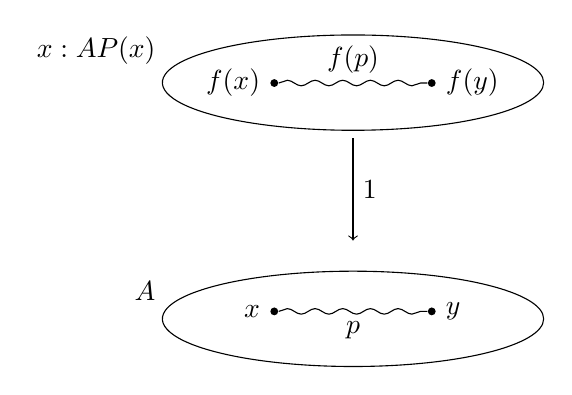
\begin{tikzpicture}[yscale=.5,xscale=2]
        \draw (0,0) arc (-90:170:8ex) node[anchor=south east] {$A$} arc (170:270:8ex);
        \draw (0,6) arc (-90:170:8ex) node[anchor=south east] {$\sm{x:A} P(x)$} arc (170:270:8ex);
        \draw[->] (0,5.8) -- node[auto] {$\proj1$} (0,3.2);
        \node[circle,fill,inner sep=1pt,label=left:{$x$}] (b1) at (-.5,1.4) {};
        \node[circle,fill,inner sep=1pt,label=right:{$y$}] (b2) at (.5,1.4) {};
        \draw[decorate,decoration={snake,amplitude=1}] (b1) -- node[auto,swap] {$p$} (b2);
        \node[circle,fill,inner sep=1pt,label=left:{$f(x)$}] (b1) at (-.5,7.2) {};
        \node[circle,fill,inner sep=1pt,label=right:{$f(y)$}] (b2) at (.5,7.2) {};
        \draw[decorate,decoration={snake,amplitude=1}] (b1) -- node[auto] {$f(p)$} (b2);
    \end{tikzpicture}
\end{center}

We \emph{can} obtain such a thing from \cref{lem:map}.
Given $f:\prd{x:A} P(x)$, we can define a non-dependent function $f':A\to \sm{x:A} P(x)$ by setting $f'(x)\defeq (x,f(x))$, and then consider $\ap{f'}{p} : f'(x) = f'(y)$.
Since $\proj1 \circ f' \jdeq \idfunc[A]$, by \cref{lem:ap-functor} we have $\ap{\proj1}{\ap{f'}{p}} = p$; thus $\ap{f'}{p}$ does ``lie over'' $p$ in this sense.
However, it is not obvious from the \emph{type} of $\ap{f'}{p}$ that it lies over any specific path in $A$ (in this case, $p$), which is sometimes important.

The solution is to use the transport lemma.
By \cref{thm:path-lifting} we have a canonical path $\mathsf{lift}(u,p)$ from $(x,u)$ to $(y,\trans p u)$ which lies over $p$.
Thus, any path from $u:P(x)$ to $v:P(y)$ lying over $p$ should factor through $\mathsf{lift}(u,p)$, essentially uniquely, by a path from $\trans p u$ to $v$ lying entirely in the fiber $P(y)$.
Thus, up to equivalence, it makes sense to define ``a path from $u$ to $v$ lying over $p:x=y$'' to mean a path $\trans p u = v$ in $P(y)$.
And, indeed, we can show that dependent functions produce such paths.

\begin{lem}[依值映射]
    \label{lem:mapdep}
    \indexdef{应用!依值函数到一个路径}%
    \indexdef{路径!依值函数的应用}%
    \indexdef{函数!依值!应用到路径}%
    \indexdef{动作!路径的依值函数的}%
    提供 $f:\prd{x: A} P(x)$; 然后有一个映射
    \[\apdfunc f : \prd{p:x=y}\big(\id[P(y)]{\trans p{f(x)}}{f(y)}\big).\]
\end{lem}

\begin{proof}[第一个证明]
    令 $D:\prd{x,y:A} (\id{x}{y}) \to \type$ 为一个如下定义的类型族
    \begin{equation*}
        D(x,y,p)\defeq \trans p {f(x)}= f(y).
    \end{equation*}
    然后 $D(x,x,\refl{x})$ 是 $\trans{(\refl{x})}{f(x)}= f(x)$.
    但是因为 $\trans{(\refl{x})}{f(x)}\jdeq f(x)$, 得到 $D(x,x,\refl{x})\jdeq (f(x)= f(x))$.
    因此, 有这个饿函数
    \begin{equation*}
        d\defeq\lam{x} \refl{f(x)}:\prd{x:A} D(x,x,\refl{x})
    \end{equation*}
    现在路径归纳给出对于每个 $p:x= y$ 有 $\apdfunc f(p):\trans p{f(x)}= f(y)$ .
\end{proof}

\begin{proof}[第二个证明]
    通过归纳, 可以假设 $p$ 是 $\refl x$.
    这个情况下, 所需的等式 $\trans{(\refl{x})}{f(x)}= f(x)$ 命题上成立.
\end{proof}

We will refer generally to paths which ``lie over other paths'' in this sense as \emph{dependent paths}.
\indexsee{dependent!path}{path, dependent}%
\index{path!dependent}%
They will play an increasingly important role starting in \cref{cha:hits}.
In \cref{sec:computational} we will see that for a few particular kinds of type families, there are equivalent ways to represent the notion of dependent paths that are sometimes more convenient.

现在回顾\cref{sec:pi-types}, 非依值类型函数 $f:A\to B$ 是依值函数 $f:\prd{x:A} P(x)$ 在 $P$ 是静态类型族 $P(x) \defeq B$ 的特殊情况.
这种情况下, $\apdfunc{f}$ 和 $\apfunc{f}$ 是密切相关的, 因为如下定理:

\begin{lem}
    \label{thm:trans-trivial}
    如果 $P:A\to\type$ 定义为 $P(x) \defeq B$ 对于固定的 $B:\type$, 那么对于任何 $x,y:A$ 和 $p:x=y$ 和 $b:B$ 有路径
    \[ \transconst Bpb : \transfib P p b = b. \]
\end{lem}
\begin{proof}[第一个证明]
    固定 $b:B$, 然后令 $D:\prd{x,y:A} (\id{x}{y}) \to \type$ 为一个类型族, 定义为
    \[ D(x,y,p) \defeq (\transfib P p b = b). \]
    然后 $D(x,x,\refl x)$ is $(\transfib P{\refl{x}}{b} = b)$, 通过运输的计算规则与 $(b=b)$ 判断等同.
    因此, 有这个函数
    \[ d \defeq \lam{x} \refl{b} : \prd{x:A} D(x,x,\refl x). \]
    现在路径归纳可以给出所需的元素
    \narrowequation{
        \prd{x,y:A}{p:x=y}(\transfib P p b = b).}
\end{proof}
\begin{proof}[第二个证明]
    通过归纳, 可以假设 $y$ 是 $x$ 而且 $p$ 是 $\refl x$.
    但是 $\transfib P {\refl x} b \jdeq b$, 所以这种情况下必须证明 $b=b$, 为此可以使用 $\refl{b}$.
\end{proof}

因此, 对于任何 $x,y:A$ 和 $p:x=y$ 和 $f:A\to B$, 通过分别连接 $\transconst Bp{f(x)}$ 和它的反转, 得到函数
\begin{align}
    \big(f(x) = f(y)\big) &\to \big(\trans{p}{f(x)} = f(y)\big)\label{eq:ap-to-apd}
    \qquad\text{和} \\
    \big(\trans{p}{f(x)} = f(y)\big) &\to \big(f(x) = f(y)\big).\label{eq:apd-to-ap}
\end{align}
事实上, 这些函数反向等价(它的意义会在\cref{sec:basics-equivalences}引入), 并且它们关联了 $\apfunc f (p)$ 和 $\apdfunc f (p)$.

\begin{lem}
    \label{thm:apd-const}
    对于 $f:A\to B$ 和 $p:\id[A]xy$, 有
    \[ \apdfunc f(p) = \transconst B p{f(x)} \ct \apfunc f (p). \]
\end{lem}
\begin{proof}[第一个证明]
    令 $D:\prd{x,y:A} (\id xy) \to \type$ 为类型族, 定义为
    \[ D(x,y,p) \defeq \big(\apdfunc f (p) = \transconst Bp{f(x)} \ct \apfunc f (p)\big). \]
    因此有
    \[D(x,x,\refl x) \jdeq \big(\apdfunc f (\refl x) = \transconst B{\refl x}{f(x)} \ct \apfunc f ({\refl x})\big).\]
    通过定义, 这个类型中出现的三个路径都是 $\refl{f(x)}$, 所以有
    \[ \refl{\refl{f(x)}} : D(x,x,\refl x). \]
    于是, 路径归纳给出所需的元素 $\prd{x,y:A}{p:x=y} D(x,y,p)$.
\end{proof}
\begin{proof}[第二个证明]
    通过归纳, 足以假定 $y$ 是 $x$ 而且 $p$ 是 $\refl x$.
    这个情况下, 需要证明的是 $\refl{f(x)} = \refl{f(x)} \ct \refl{f(x)}$, 判断上为真.
\end{proof}

因为 $\apdfunc{f}$ 和 $\apfunc{f}$ 的类型不同, 使用不同的符号会更清晰.
% We may sometimes use a notation $\apd f p$ for $\apdfunc{f}(p)$, which is similar to the notation $\ap f p$ for $\apfunc{f}(p)$.

\index{函数!依值|)}%

至此, 希望读者开始找到一些通过恒等类型的归纳做证明的感觉.
从现在开始不再给出两种风格的证明, 而是使用更清晰和使用的 (大部分情况是更简明的第二种).
这里有一些实用的运输定理; 留给读者做证明 (用两种风格).

\begin{lem}
    \label{thm:transport-concat}
    给定 $P:A\to\type$ 和 $p:\id[A]xy$ 与 $q:\id[A]yz$ 并且 $u:P(x)$, 有
    \[ \trans{q}{\trans{p}{u}} = \trans{(p\ct q)}{u}. \]
\end{lem}

\begin{lem}
    \label{thm:transport-compose}
    对于函数 $f:A\to B$ 和类型族 $P:B\to\type$, 和任意 $p:\id[A]xy$ 与 $u:P(f(x))$, 有
    \[ \transfib{P\circ f}{p}{u} = \transfib{P}{\apfunc f(p)}{u}. \]
\end{lem}

\begin{lem}
    \label{thm:ap-transport}
    对于 $P,Q:A\to \type$ 和函数的族 $f:\prd{x:A} P(x)\to Q(x)$, 和任意 $p:\id[A]xy$ 与 $u:P(x)$, 有
    \[ \transfib{Q}{p}{f_x(u)} = f_y(\transfib{P}{p}{u}). \]
\end{lem}

\index{type!family of|)}%
\index{transport|)}

\section{Homotopies and equivalences}
\label{sec:basics-equivalences}
\index{homotopy|(defstyle}%

So far, we have seen how the identity type $\id[A]xy$ can be regarded as a type of \emph{identifications}, \emph{paths}, or \emph{equivalences} between two elements $x$ and~$y$ of a type $A$.
Now we investigate the appropriate notions of ``identification'' or ``sameness'' between \emph{functions} and between \emph{types}.
In \cref{sec:compute-pi,sec:compute-universe}, we will see that homotopy type theory allows us to identify these with instances of the identity type, but before we can do that we need to understand them in their own right.

Traditionally, we regard two functions as the same if they take equal values on all inputs.
Under the propositions-as-types interpretation, this suggests that two functions $f$ and $g$ (perhaps dependently typed) should be the same if the type $\prd{x:A} (f(x)=g(x))$ is inhabited.
Under the homotopical interpretation, this dependent function type consists of \emph{continuous} paths or \emph{functorial} equivalences, and thus may be regarded as the type of \emph{homotopies} or of \emph{natural isomorphisms}.\index{isomorphism!natural}
We will adopt the topological terminology for this.

\begin{defn} \label{defn:homotopy}
  Let $f,g:\prd{x:A} P(x)$ be two sections of a type family $P:A\to\type$.
  A \define{homotopy}
  from $f$ to $g$ is a dependent function of type
  \begin{equation*}
    (f\htpy g) \defeq \prd{x:A} (f(x)=g(x)).
  \end{equation*}
\end{defn}

Note that a homotopy is not the same as an identification $(f=g)$.
However, in \cref{sec:compute-pi} we will introduce an axiom making homotopies and identifications ``equivalent''.

The following proofs are left to the reader.

\begin{lem}\label{lem:homotopy-props}
  Homotopy is an equivalence relation on each dependent function type $\prd{x:A} P(x)$.
  That is, we have elements of the types
  \begin{gather*}
    \prd{f:\prd{x:A} P(x)} (f\htpy f)\\
    \prd{f,g:\prd{x:A} P(x)} (f\htpy g) \to (g\htpy f)\\
    \prd{f,g,h:\prd{x:A} P(x)} (f\htpy g) \to (g\htpy h) \to (f\htpy h).
  \end{gather*}
\end{lem}

% This is judgmental and is \cref{ex:composition}.
% \begin{lem}
%   Composition is associative and unital up to homotopy.
%   That is:
%   \begin{enumerate}
%   \item If $f:A\to B$ then $f\circ \idfunc[A]\htpy f\htpy \idfunc[B]\circ f$.
%   \item If $f:A\to B, g:B\to C$ and $h:C\to D$ then $h\circ (g\circ f) \htpy (h\circ g)\circ f$.
%   \end{enumerate}
% \end{lem}

\index{functoriality of functions in type theory@``functoriality'' of functions in type theory}%
\index{continuity of functions in type theory@``continuity'' of functions in type theory}%
Just as functions in type theory are automatically ``functors'', homotopies are automatically
\index{naturality of homotopies@``naturality'' of homotopies}%
``natural transformations''.
We will state and prove this only for non-dependent functions $f,g:A\to B$; in \cref{ex:dep-htpy-natural} we ask the reader to generalize it to dependent functions.

Recall that for $f:A\to B$ and $p:\id[A]xy$, we may write $\ap f p$ to mean $\apfunc{f} (p)$.

\begin{lem}\label{lem:htpy-natural}
  Suppose $H:f\htpy g$ is a homotopy between functions $f,g:A\to B$ and let $p:\id[A]xy$.  Then we have
  \begin{equation*}
    H(x)\ct\ap{g}{p}=\ap{f}{p}\ct H(y).
  \end{equation*}
  We may also draw this as a commutative diagram:\index{diagram}
  \begin{align*}
    \xymatrix{
      f(x) \ar@{=}[r]^{\ap fp} \ar@{=}[d]_{H(x)} & f(y) \ar@{=}[d]^{H(y)} \\
      g(x) \ar@{=}[r]_{\ap gp} & g(y)
    }
  \end{align*}
\end{lem}
\begin{proof}
  By induction, we may assume $p$ is $\refl x$.
  Since $\apfunc{f}$ and $\apfunc g$ compute on reflexivity, in this case what we must show is
  \[ H(x) \ct \refl{g(x)} = \refl{f(x)} \ct H(x). \]
  But this follows since both sides are equal to $H(x)$.
\end{proof}

\begin{cor}\label{cor:hom-fg}
  Let $H : f \htpy \idfunc[A]$ be a homotopy, with $f : A \to A$. Then for any $x : A$ we have \[ H(f(x)) = \ap f{H(x)}. \]
  % The above path will be denoted by $\com{H}{f}{x}$.
\end{cor}
\noindent
Here $f(x)$ denotes the ordinary application of $f$ to $x$, while $\ap f{H(x)}$ denotes $\apfunc{f}(H(x))$.
\begin{proof}
By naturality of $H$, the following diagram of paths commutes:
\begin{align*}
\xymatrix@C=3pc{
ffx \ar@{=}[r]^-{\ap f{Hx}} \ar@{=}[d]_{H(fx)} & fx \ar@{=}[d]^{Hx} \\
fx \ar@{=}[r]_-{Hx} & x
}
\end{align*}
That is, $\ap f{H x} \ct H x = H(f x) \ct H x$.
We can now whisker by $\opp{(H x)}$ to cancel $H x$, obtaining
\[ \ap f{H x}
= \ap f{H x} \ct H x \ct \opp{(H x)}
= H(f x) \ct H x \ct \opp{(H x)}
= H(f x)
\]
as desired (with some associativity paths suppressed).
\end{proof}

Of course, like the functoriality of functions (\cref{lem:ap-functor}), the equality in \cref{lem:htpy-natural} is a path which satisfies its own coherence laws, and so on.

\index{homotopy|)}%

\index{equivalence|(}%
Moving on to types, from a traditional perspective one may say that a function $f:A\to B$ is an \emph{isomorphism} if there is a function $g:B\to A$ such that both composites $f\circ g$ and $g\circ f$ are pointwise equal to the identity, i.e.\ such that $f \circ g \htpy \idfunc[B]$ and $g\circ f \htpy \idfunc[A]$.
\indexsee{homotopy!equivalence}{equivalence}%
A homotopical perspective suggests that this should be called a \emph{homotopy equivalence}, and from a categorical one, it should be called an \emph{equivalence of (higher) groupoids}.
However, when doing proof-relevant mathematics,
\index{mathematics!proof-relevant}%
the corresponding type
\begin{equation}
  \sm{g:B\to A} \big((f \circ g \htpy \idfunc[B]) \times (g\circ f \htpy \idfunc[A])\big)\label{eq:qinvtype}
\end{equation}
is poorly behaved.
For instance, for a single function $f:A\to B$ there may be multiple unequal inhabitants of~\eqref{eq:qinvtype}.
(This is closely related to the observation in higher category theory that often one needs to consider \emph{adjoint} equivalences\index{adjoint!equivalence} rather than plain equivalences.)
For this reason, we give~\eqref{eq:qinvtype} the following historically accurate, but slightly de\-rog\-a\-to\-ry-sounding name instead.

\begin{defn}\label{defn:quasi-inverse}
  For a function $f:A\to B$, a \define{quasi-inverse}
  \indexdef{quasi-inverse}%
  \indexsee{function!quasi-inverse of}{quasi-inverse}%
  of $f$ is a triple $(g,\alpha,\beta)$ consisting of a function $g:B\to A$ and homotopies
$\alpha:f\circ g\htpy \idfunc[B]$ and $\beta:g\circ f\htpy \idfunc[A]$.
\end{defn}

\symlabel{qinv}
Thus,~\eqref{eq:qinvtype} is \emph{the type of quasi-inverses of $f$}; we may denote it by $\qinv(f)$.

\begin{eg}\label{eg:idequiv}
  \index{identity!function}%
  \index{function!identity}%
  The identity function $\idfunc[A]:A\to A$ has a quasi-inverse given by $\idfunc[A]$ itself, together with homotopies defined by $\alpha(y) \defeq \refl{y}$ and $\beta(x) \defeq \refl{x}$.
\end{eg}

\begin{eg}\label{eg:concatequiv}
  For any $p:\id[A]xy$ and $z:A$, the functions
  \begin{align*}
    (p\ct \blank)&:(\id[A]yz) \to (\id[A]xz) \qquad\text{and}\\
    (\blank \ct p)&:(\id[A]zx) \to (\id[A]zy)
  \end{align*}
  have quasi-inverses given by $(\opp p \ct \blank)$ and $(\blank \ct \opp p)$, respectively; see \cref{ex:equiv-concat}.
\end{eg}

\begin{eg}\label{thm:transportequiv}
  For any $p:\id[A]xy$ and $P:A\to\type$, the function
  \[\transfib{P}{p}{\blank}:P(x) \to P(y)\]
  has a quasi-inverse given by $\transfib{P}{\opp p}{\blank}$; this follows from \narrowbreak \cref{thm:transport-concat}.
\end{eg}

\symlabel{basics-isequiv}\symlabel{basics:iso}
In general, we will only use the word \emph{isomorphism}
\index{isomorphism!of sets}
(and similar words such as \emph{bijection}, and the associated notation $A\cong B$)
\index{bijection}
in the special case when the types $A$ and $B$ ``behave like sets'' (see \cref{sec:basics-sets}).
In this case, the type~\eqref{eq:qinvtype} is unproblematic.
We will reserve the word \emph{equivalence} for an improved notion $\isequiv (f)$ with the following properties:%
\begin{enumerate}
\item For each $f:A\to B$ there is a function $\qinv(f) \to \isequiv (f)$.\label{item:be1}
\item Similarly, for each $f$ we have $\isequiv (f) \to \qinv(f)$; thus the two are logically equivalent (see \cref{sec:pat}).\label{item:be2}
\item For any two inhabitants $e_1,e_2:\isequiv(f)$ we have $e_1=e_2$.\label{item:be3}
\end{enumerate}
In \cref{cha:equivalences} we will see that there are many different definitions of $\isequiv(f)$ which satisfy these three properties, but that all of them are equivalent.
For now, to convince the reader that such things exist, we mention only the easiest such definition:
\begin{equation}\label{eq:isequiv-invertible}
  \isequiv(f) \;\defeq\;
  \Parens{\sm{g:B\to A} (f\circ g \htpy \idfunc[B])}
  \times
  \Parens{\sm{h:B\to A} (h\circ f \htpy \idfunc[A])}.
\end{equation}
We can show~\ref{item:be1} and~\ref{item:be2} for this definition now.
A function $\qinv(f) \to \isequiv (f)$ is easy to define by taking $(g,\alpha,\beta)$ to $(g,\alpha,g,\beta)$.
In the other direction, given $(g,\alpha,h,\beta)$, let $\gamma$ be the composite homotopy
\[ g \overset{\beta}{\htpy} h\circ f\circ g \overset{\alpha}{\htpy} h, \]
meaning that $\gamma(x) \defeq \opp{\beta(g(x))} \ct \ap{h}{\alpha(x)}$.
Now define $\beta':g\circ f\htpy \idfunc[A]$ by $\beta'(x) \defeq \gamma(f(x)) \ct \beta(x)$.
Then $(g,\alpha,\beta'):\qinv(f)$.

Property~\ref{item:be3} for this definition is not too hard to prove either, but it requires identifying the identity types of cartesian products and dependent pair types, which we will discuss in \cref{sec:compute-cartprod,sec:compute-sigma}.
Thus, we postpone it as well; see \cref{sec:biinv}.
At this point, the main thing to take away is that there is a well-behaved type which we can pronounce as ``$f$ is an equivalence'', and that we can prove $f$ to be an equivalence by exhibiting a quasi-inverse to it.
In practice, this is the most common way to prove that a function is an equivalence.

In accord with the proof-relevant philosophy,
\index{mathematics!proof-relevant}%
\emph{an equivalence} from $A$ to $B$ is defined to be a function $f:A\to B$ together with an inhabitant of $\isequiv (f)$, i.e.\ a proof that it is an equivalence.
We write $(\eqv A B)$ for the type of equivalences from $A$ to $B$, i.e.\ the type
\begin{equation}\label{eq:eqv}
  (\eqv A B) \defeq \sm{f:A\to B} \isequiv(f).
\end{equation}
Property~\ref{item:be3} above will ensure that if two equivalences are equal as functions (that is, the underlying elements of $A\to B$ are equal), then they are also equal as equivalences (see \cref{sec:compute-sigma}).
Thus, we often abuse notation and blur the distinction between equivalences and their underlying functions.
For instance, if we have a function $f:A\to B$ and we know that $e:\isequiv(f)$, we may write $f:\eqv A B$, rather than $\tup{f}{e}$.
Or conversely, if we have an equivalence $g:\eqv A B$, we may write $g(a)$ when given $a:A$, rather than $(\proj1 g)(a)$.

We conclude by observing:

\begin{lem}\label{thm:equiv-eqrel}
  Type equivalence is an equivalence relation on \type.
  More specifically:
  \begin{enumerate}
  \item For any $A$, the identity function $\idfunc[A]$ is an equivalence; hence $\eqv A A$.
  \item For any $f:\eqv A B$, we have an equivalence $f^{-1} : \eqv B A$.
  \item For any $f:\eqv A B$ and $g:\eqv B C$, we have $g\circ f : \eqv A C$.
  \end{enumerate}
\end{lem}
\begin{proof}
  The identity function is clearly its own quasi-inverse; hence it is an equivalence.

  If $f:A\to B$ is an equivalence, then it has a quasi-inverse, say $f^{-1}:B\to A$.
  Then $f$ is also a quasi-inverse of $f^{-1}$, so $f^{-1}$ is an equivalence $B\to A$.

  Finally, given $f:\eqv A B$ and $g:\eqv B C$ with quasi-inverses $f^{-1}$ and $g^{-1}$, say, then for any $a:A$ we have $f^{-1} g^{-1} g f a = f^{-1} f a = a$, and for any $c:C$ we have $g f f^{-1} g^{-1} c = g g^{-1} c = c$.
  Thus $f^{-1} \circ g^{-1}$ is a quasi-inverse to $g\circ f$, hence the latter is an equivalence.
\end{proof}

\index{equivalence|)}%

\section{The higher groupoid structure of type formers}
\label{sec:computational}
In \cref{cha:typetheory}, we introduced many ways to form new types: cartesian products, disjoint unions, dependent products, dependent sums, etc.
In \cref{sec:equality,sec:functors,sec:fibrations}, we saw that \emph{all} types in homotopy type theory behave like spaces or higher groupoids.
Our goal in the rest of the chapter is to make explicit how this higher structure behaves in the case of the particular types defined in \cref{cha:typetheory}.

It turns out that for many types $A$, the equality types $\id[A]xy$ can be characterized, up to equivalence, in terms of whatever data was used to construct $A$.
For example, if $A$ is a cartesian product $B\times C$, and $x\jdeq (b,c)$ and $y\jdeq(b',c')$, then we have an equivalence
\begin{equation}\label{eq:prodeqv}
  \eqv{\big((b,c)=(b',c')\big)}{\big((b=b')\times (c=c')\big)}.
\end{equation}
In more traditional language, two ordered pairs are equal just when their components are equal (but the equivalence~\eqref{eq:prodeqv} says rather more than this).
The higher structure of the identity types can also be expressed in terms of these equivalences; for instance, concatenating two equalities between pairs corresponds to pairwise concatenation.

Similarly, when a type family $P:A\to\type$ is built up fiberwise using the type forming rules from \cref{cha:typetheory}, the operation $\transfib{P}{p}{\blank}$ can be characterized, up to homotopy, in terms of the corresponding operations on the data that went into $P$.
For instance, if $P(x) \jdeq B(x)\times C(x)$, then we have
\[\transfib{P}{p}{(b,c)} = \big(\transfib{B}{p}{b},\transfib{C}{p}{c}\big).\]

Finally, the type forming rules are also functorial, and if a function $f$ is built from this functoriality, then the operations $\apfunc f$ and $\apdfunc f$ can be computed based on the corresponding ones on the data going into $f$.
For instance, if $g:B\to B'$ and $h:C\to C'$ and we define $f:B\times C \to B'\times C'$ by $f(b,c)\defeq (g(b),h(c))$, then modulo the equivalence~\eqref{eq:prodeqv}, we can identify $\apfunc f$ with ``$(\apfunc g,\apfunc h)$''.

The next few sections (\crefrange{sec:compute-cartprod}{sec:compute-nat}) will be devoted to stating and proving theorems of this sort for all the basic type forming rules, with one section for each basic type former.
Here we encounter a certain apparent deficiency in currently available type theories;
as will become clear in later chapters, it would seem to be more convenient and intuitive if these characterizations of identity types, transport, and so on were \emph{judgmental}\index{judgmental equality} equalities.
However, in the theory presented in \cref{cha:typetheory}, the identity types are defined uniformly for all types by their induction principle, so we cannot ``redefine'' them to be different things at different types.
Thus, the characterizations for particular types to be discussed in this chapter are, for the most part, \emph{theorems} which we have to discover and prove, if possible.

Actually, the type theory of \cref{cha:typetheory} is insufficient to prove the desired theorems for two of the type formers: $\Pi$-types and universes.
For this reason, we are forced to introduce axioms into our type theory, in order to make those ``theorems'' true.
Type-theoretically, an \emph{axiom} (c.f.~\cref{sec:axioms}) is an ``atomic'' element that is declared to inhabit some specified type, without there being any rules governing its behavior other than those pertaining to the type it inhabits.
\index{axiom!versus rules}%

\index{function extensionality}%
\indexsee{extensionality, of functions}{function extensionality}
\index{univalence axiom}%
The axiom for $\Pi$-types (\cref{sec:compute-pi}) is familiar to type theorists: it is called \emph{function extensionality}, and states (roughly) that if two functions are homotopic in the sense of \cref{sec:basics-equivalences}, then they are equal.
The axiom for universes (\cref{sec:compute-universe}), however, is a new contribution of homotopy type theory due to Voevodsky: it is called the \emph{univalence axiom}, and states (roughly) that if two types are equivalent in the sense of \cref{sec:basics-equivalences}, then they are equal.
We have already remarked on this axiom in the introduction; it will play a very important role in this book.%
\footnote{We have chosen to introduce these principles as axioms, but there are potentially other ways to formulate a type theory in which they hold.
  See the Notes to this chapter.}

It is important to note that not \emph{all} identity types can be ``determined'' by induction over the construction of types.
Counterexamples include most nontrivial higher inductive types (see \cref{cha:hits,cha:homotopy}).
For instance, calculating the identity types of the types $\Sn^n$ (see \cref{sec:circle}) is equivalent to calculating the higher homotopy groups of spheres, a deep and important field of research in algebraic topology.

\section{Cartesian product types}
\label{sec:compute-cartprod}
\index{type!product|(}%
Given types $A$ and $B$, consider the cartesian product type $A \times B$.
For any elements $x,y:A\times B$ and a path $p:\id[A\times B]{x}{y}$, by functoriality we can extract paths $\ap{\proj1}p:\id[A]{\proj1(x)}{\proj1(y)}$ and $\ap{\proj2}p:\id[B]{\proj2(x)}{\proj2(y)}$.
Thus, we have a function
\begin{equation}\label{eq:path-prod}
  (\id[A\times B]{x}{y}) \to (\id[A]{\proj1(x)}{\proj1(y)}) \times (\id[B]{\proj2(x)}{\proj2(y)}).
\end{equation}

\begin{thm}\label{thm:path-prod}
  For any $x$ and $y$, the function~\eqref{eq:path-prod} is an equivalence.
\end{thm}

Read logically, this says that two pairs are equal just if they are equal
componentwise.  Read category-theoretically, this says that the
morphisms in a product groupoid are pairs of morphisms.  Read
homotopy-theoretically, this says that the paths in a product
space are pairs of paths.

\begin{proof}
  We need a function in the other direction:
  \begin{equation}
    (\id[A]{\proj1(x)}{\proj1(y)}) \times (\id[B]{\proj2(x)}{\proj2(y)}) \to (\id[A\times B]{x}{y}). \label{eq:path-prod-inverse}
  \end{equation}
  By the induction rule for cartesian products, we may assume that $x$ and $y$ are both pairs, i.e.\ $x\jdeq (a,b)$ and $y\jdeq (a',b')$ for some $a,a':A$ and $b,b':B$.
  In this case, what we want is a function
  \begin{equation*}
    (\id[A]{a}{a'}) \times (\id[B]{b}{b'}) \to \big(\id[A\times B]{(a,b)}{(a',b')}\big).
  \end{equation*}
  Now by induction for the cartesian product in its domain, we may assume given $p:a=a'$ and $q:b=b'$.
  And by two path inductions, we may assume that $a\jdeq a'$ and $b\jdeq b'$ and both $p$ and $q$ are reflexivity.
  But in this case, we have $(a,b)\jdeq(a',b')$ and so we can take the output to also be reflexivity.

  It remains to prove that~\eqref{eq:path-prod-inverse} is quasi-inverse to~\eqref{eq:path-prod}.
  This is a simple sequence of inductions, but they have to be done in the right order.

  In one direction, let us start with $r:\id[A\times B]{x}{y}$.
  We first do a path induction on $r$ in order to assume that $x\jdeq y$ and $r$ is reflexivity.
  In this case, since $\apfunc{\proj1}$ and $\apfunc{\proj2}$ are defined by path induction,~\eqref{eq:path-prod} takes $r\jdeq \refl{x}$ to the pair $(\refl{\proj1x},\refl{\proj2x})$.
  Now by induction on $x$, we may assume $x\jdeq (a,b)$, so that this is $(\refl a, \refl b)$.
  Thus,~\eqref{eq:path-prod-inverse} takes it by definition to $\refl{(a,b)}$, which (under our current assumptions) is $r$.

  In the other direction, if we start with $s:(\id[A]{\proj1(x)}{\proj1(y)}) \times (\id[B]{\proj2(x)}{\proj2(y)})$, then we first do induction on $x$ and $y$ to assume that they are pairs $(a,b)$ and $(a',b')$, and then induction on $s:(\id[A]{a}{a'}) \times (\id[B]{b}{b'})$ to reduce it to a pair $(p,q)$ where $p:a=a'$ and $q:b=b'$.
  Now by induction on $p$ and $q$, we may assume they are reflexivities $\refl a$ and $\refl b$, in which case~\eqref{eq:path-prod-inverse} yields $\refl{(a,b)}$ and then~\eqref{eq:path-prod} returns us to $(\refl a,\refl b)\jdeq (p,q)\jdeq s$.
\end{proof}

In particular, we have shown that~\eqref{eq:path-prod} has an inverse~\eqref{eq:path-prod-inverse}, which we may denote by
\symlabel{defn:pairpath}
\[
\pairpath : (\id{\proj{1}(x)}{\proj{1}(y)}) \times (\id{\proj{2}(x)}{\proj{2}(y)}) \to (\id x y).
\]
Note that a special case of this yields the propositional uniqueness principle\index{uniqueness!principle, propositional!for product types} for products: $z = (\proj1(z),\proj2(z))$.

It can be helpful to view \pairpath as a \emph{constructor} or \emph{introduction rule} for $\id x y$, analogous to the ``pairing'' constructor of $A\times B$ itself, which introduces the pair $(a,b)$ given $a:A$ and $b:B$.
From this perspective, the two components of~\eqref{eq:path-prod}:
\begin{align*}
  \projpath{1} &: (\id{x}{y}) \to (\id{\proj{1}(x)}{\proj{1} (y)})\\
  \projpath{2} &: (\id{x}{y}) \to (\id{\proj{2}(x)}{\proj{2} (y)})
\end{align*}
are \emph{elimination} rules.
Similarly, the two homotopies which witness~\eqref{eq:path-prod-inverse} as quasi-inverse to~\eqref{eq:path-prod} consist, respectively, of \emph{propositional computation rules}:
\index{computation rule!propositional!for identities between pairs}%
\begin{align*}
  {\projpath{1}{(\pairpath(p, q)})}
  &= %_{(\id{\proj{1} x}{\proj{1} y})}
  {p} \\
  {\projpath{2}{(\pairpath(p,q)})}
  &= %_{(\id{\proj{2} x}{\proj{2} y})}
  {q}
\end{align*}
for $p:\id{\proj{1} x}{\proj{1} y}$ and $q:\id{\proj{2} x}{\proj{2} y}$,
and a \emph{propositional uniqueness principle}:
\index{uniqueness!principle, propositional!for identities between pairs}%
\[
\id{r}{\pairpath(\projpath{1} (r), \projpath{2} (r)) }
\qquad\text{for } r : \id[A \times B] x y.
\]

We can also characterize the reflexivity, inverses, and composition of paths in $A\times B$ componentwise:
\begin{align*}
  {\refl{(z : A \times B)}}
  &= {\pairpath (\refl{\proj{1} z},\refl{\proj{2} z})} \\
  {\opp{p}}
  &= {\pairpath \big(\opp{\projpath{1} (p)},\, \opp{\projpath{2} (p)}\big)} \\
  {{p \ct q}}
  &= {\pairpath \big({\projpath{1} (p)} \ct {\projpath{1} (q)},\,{\projpath{2} (p)} \ct {\projpath{2} (q)}\big)}.
\end{align*}
Or, written differently:
\begin{alignat*}{2}
  \projpath{i}(\refl{(z : A \times B)}) &= \refl{\proj{i} z} &\qquad (i=1,2)\\
  \pairpath(\opp p, \opp q) &= \opp{\pairpath(p,q)}\\
  \pairpath(p\ct q, p'\ct q') &= \pairpath(p,p') \ct \pairpath(q,q').
\end{alignat*}
All of these equations can be derived by using path induction on the given paths and then returning reflexivity.
The same is true for the rest of the higher groupoid structure considered in \cref{sec:equality}, although it begins to get tedious to insert enough other coherence paths to yield an equation that will typecheck.
For instance, if we denote the inverse of the path in \cref{thm:omg}\ref{item:omg4} by $\ctassoc(p,q,r)$ and the last path displayed above by $\pairct(p,q,p',q')$, then for any $u,v,z,w:A\times B$ and $p,q,r,p',q',r'$ of appropriate types we have
\begin{equation*}
  \begin{array}{l}
    \pairct(p\ct q, r, p'\ct q', r') \\
    \ct\;  (\pairct(p,q,p',q') \rightwhisker \pairpath(r,r')) \\
    \ct\;  \ctassoc(\pairpath(p,p'),\pairpath(q,q'),\pairpath(r,r'))\\
    =
    \begin{array}[t]{l}
      \apfunc{\pairpath}({\pairpath(\ctassoc(p,q,r),\ctassoc(p',q',r'))})\\
      \ct\; \pairct(p, q\ct r, p', q'\ct r')\\
      \ct\; (\pairpath(p,p') \leftwhisker \pairct(q,r,q',r')).
    \end{array}
  \end{array}
\end{equation*}
Fortunately, we will never have to use any such higher-dimensional coherences.

\index{transport!in product types}%
We now consider transport in a pointwise product of type families.
Given type families $ A, B : Z \to \type$, we abusively write $A\times B:Z\to \type$ for the type family defined by $(A\times B)(z) \defeq A(z) \times B(z)$.
Now given $p : \id[Z]{z}{w}$ and $x : A(z) \times B(z)$, we can transport $x$ along $p$ to obtain an element of $A(w)\times B(w)$.

\begin{thm}\label{thm:trans-prod}
  In the above situation, we have
  \[
  \id[A(w) \times B(w)]
  {\transfib{A\times B}px}
  {(\transfib{A}{p}{\proj{1}x}, \transfib{B}{p}{\proj{2}x})}.
  \]
\end{thm}
\begin{proof}
  By path induction, we may assume $p$ is reflexivity, in which case we have
  \begin{align*}
    \transfib{A\times B}px&\jdeq x\\
    \transfib{A}{p}{\proj{1}x}&\jdeq \proj1x\\
    \transfib{B}{p}{\proj{2}x}&\jdeq \proj2x.
  \end{align*}
  Thus, it remains to show $x = (\proj1 x, \proj2x)$.
  But this is the propositional uniqueness principle for product types, which, as we remarked above, follows from \cref{thm:path-prod}.
\end{proof}

Finally, we consider the functoriality of $\apfunc{}$ under cartesian products.
Suppose given types $A,B,A',B'$ and functions $g:A\to A'$ and $h:B\to B'$; then we can define a function $f:A\times B\to A'\times B'$ by $f(x) \defeq (g(\proj1x),h(\proj2x))$.

\begin{thm}\label{thm:ap-prod}
  In the above situation, given $x,y:A\times B$ and $p:\proj1x=\proj1y$ and $q:\proj2x=\proj2y$, we have
  \[ \id[(f(x)=f(y))]{\ap{f}{\pairpath(p,q)}} {\pairpath(\ap{g}{p},\ap{h}{q})}. \]
\end{thm}
\begin{proof}
  Note first that the above equation is well-typed.
  On the one hand, since $\pairpath(p,q):x=y$ we have $\ap{f}{\pairpath(p,q)}:f(x)=f(y)$.
  On the other hand, since $\proj1(f(x))\jdeq g(\proj1x)$ and $\proj2(f(x))\jdeq h(\proj2x)$, we also have $\pairpath(\ap{g}{p},\ap{h}{q}):f(x)=f(y)$.

  Now, by induction, we may assume $x\jdeq(a,b)$ and $y\jdeq(a',b')$, in which case we have $p:a=a'$ and $q:b=b'$.
  Thus, by path induction, we may assume $p$ and $q$ are reflexivity, in which case the desired equation holds judgmentally.
\end{proof}

\index{type!product|)}%

\section{\texorpdfstring{$\Sigma$}{Σ}-types}
\label{sec:compute-sigma}
\index{type!dependent pair|(}%
Let $A$ be a type and $P:A\to\type$ a type family.
Recall that the $\Sigma$-type, or dependent pair type, $\sm{x:A} P(x)$ is a generalization of the cartesian product type.
Thus, we expect its higher groupoid structure to also be a generalization of the previous section.
In particular, its paths should be pairs of paths, but it takes a little thought to give the correct types of these paths.

Suppose that we have a path $p:w=w'$ in $\sm{x:A}P(x)$.
Then we get $\ap{\proj{1}}{p}:\proj{1}(w)=\proj{1}(w')$.
However, we cannot directly ask whether $\proj{2}(w)$ is identical to $\proj{2}(w')$ since they don't have to be in the same type.
But we can transport\index{transport} $\proj{2}(w)$ along the path $\ap{\proj{1}}{p}$, and this does give us an element of the same type as $\proj{2}(w')$.
By path induction, we do in fact obtain a path $\trans{\ap{\proj{1}}{p}}{\proj{2}(w)}=\proj{2}(w')$.

Recall from the discussion preceding \cref{lem:mapdep} that
\narrowequation{
  \trans{\ap{\proj{1}}{p}}{\proj{2}(w)}=\proj{2}(w')
}
can be regarded as the type of paths from $\proj2(w)$ to $\proj2(w')$ which lie over the path $\ap{\proj1}{p}$ in $A$.
\index{fibration}%
\index{total!space}%
Thus, we are saying that a path $w=w'$ in the total space determines (and is determined by) a path $p:\proj1(w)=\proj1(w')$ in $A$ together with a path from $\proj2(w)$ to $\proj2(w')$ lying over $p$, which seems sensible.

\begin{rmk}
  Note that if we have $x:A$ and $u,v:P(x)$ such that $(x,u)=(x,v)$, it does not follow that $u=v$.
  All we can conclude is that there exists $p:x=x$ such that $\trans p u = v$.
  This is a well-known source of confusion for newcomers to type theory, but it makes sense from a topological viewpoint: the existence of a path $(x,u)=(x,v)$ in the total space of a fibration between two points that happen to lie in the same fiber does not imply the existence of a path $u=v$ lying entirely \emph{within} that fiber.
\end{rmk}

The next theorem states that we can also reverse this process.
Since it is a direct generalization of \cref{thm:path-prod}, we will be more concise.

\begin{thm}\label{thm:path-sigma}
Suppose that $P:A\to\type$ is a type family over a type $A$ and let $w,w':\sm{x:A}P(x)$. Then there is an equivalence
\begin{equation*}
\eqvspaced{(w=w')}{\dsm{p:\proj{1}(w)=\proj{1}(w')} \trans{p}{\proj{2}(w)}=\proj{2}(w')}.
\end{equation*}
\end{thm}

\begin{proof}
We define a function
\begin{equation*}
f : \prd{w,w':\sm{x:A}P(x)} (w=w') \to \dsm{p:\proj{1}(w)=\proj{1}(w')} \trans{p}{\proj{2}(w)}=\proj{2}(w')
\end{equation*}
by path induction, with
\begin{equation*}
f(w,w,\refl{w})\defeq(\refl{\proj{1}(w)},\refl{\proj{2}(w)}).
\end{equation*}
We want to show that $f$ is an equivalence.

In the reverse direction, we define
\begin{narrowmultline*}
  g : \prd{w,w':\sm{x:A}P(x)}
      \Parens{\sm{p:\proj{1}(w)=\proj{1}(w')}\trans{p}{\proj{2}(w)}=\proj{2}(w')}
      \to
      \narrowbreak
      (w=w')
\end{narrowmultline*}
by first inducting on $w$ and $w'$, which splits them into $(w_1,w_2)$ and
$(w_1',w_2')$ respectively, so it suffices to show
\begin{equation*}
\Parens{\sm{p:w_1 = w_1'}\trans{p}{w_2}=w_2'} \to ((w_1,w_2)=(w_1',w_2')).
\end{equation*}
Next, given a pair $\sm{p:w_1 = w_1'}\trans{p}{w_2}=w_2'$, we can
use $\Sigma$-induction to get $p : w_1 = w_1'$ and $q :
\trans{p}{w_2}=w_2'$.  Inducting on $p$, we have $q :
\trans{(\refl{w_1})}{w_2}=w_2'$, and it suffices to show
$(w_1,w_2)=(w_1,w_2')$.  But $\trans{(\refl{w_1})}{w_2} \jdeq w_2$, so
inducting on $q$ reduces the goal to
$(w_1,w_2)=(w_1,w_2)$, which we can prove with $\refl{(w_1,w_2)}$.

Next we show that $f(g(r))=r$ for all $w$, $w'$ and
$r$, where $r$ has type
\[\dsm{p:\proj{1}(w)=\proj{1}(w')} (\trans{p}{\proj{2}(w)}=\proj{2}(w')).\]
First, we break apart the pairs $w$, $w'$, and $r$ by pair induction, as in the
definition of $g$, and then use two path inductions to reduce both components
of $r$ to \refl{}.  Then it suffices to show that
$f (g(\refl{w_1},\refl{w_2})) = (\refl{w_1},\refl{w_2})$, which is true by definition.

Similarly, to show that $g(f(p))=p$ for all $w$, $w'$,
and $p : w = w'$, we can do path induction on $p$, and then pair induction to
split $w$, at which point it suffices to show that
$g(f (\refl{(w_1,w_2)})) = \refl{(w_1,w_2)}$, which is true by
definition.

Thus, $f$ has a quasi-inverse, and is therefore an equivalence.
\end{proof}

As we did in the case of cartesian products, we can deduce a propositional uniqueness principle as a special case.

\begin{cor}\label{thm:eta-sigma}
  \index{uniqueness!principle, propositional!for dependent pair types}%
  For $z:\sm{x:A} P(x)$, we have $z = (\proj1(z),\proj2(z))$.
\end{cor}
\begin{proof}
  We have $\refl{\proj1(z)} : \proj1(z) = \proj1(\proj1(z),\proj2(z))$, so by \cref{thm:path-sigma} it will suffice to exhibit a path $\trans{(\refl{\proj1(z)})}{\proj2(z)} = \proj2(\proj1(z),\proj2(z))$.
  But both sides are judgmentally equal to $\proj2(z)$.
\end{proof}

Like with binary cartesian products, we can think of
the backward direction of \cref{thm:path-sigma} as
an introduction form (\pairpath{}{}), the forward direction as
elimination forms (\projpath{1} and \projpath{2}), and the equivalence
as giving a propositional computation rule and uniqueness principle for these.

Note that the lifted path $\mathsf{lift}(u,p)$  of $p:x=y$ at $u:P(x)$ defined in \cref{thm:path-lifting} may be identified with the special case of the introduction form
\[\pairpath(p,\refl{\trans p u}):(x,u) = (y,\trans p u).\]
\index{transport!in dependent pair types}%
This appears in the statement of action of transport on $\Sigma$-types, which is also a generalization of the action for binary cartesian products:

\begin{thm}\label{transport-Sigma}
  Suppose we have type families
  %
  \begin{equation*}
    P:A\to\type
    \qquad\text{and}\qquad
    Q:\Parens{\sm{x:A} P(x)}\to\type.
  \end{equation*}
  %
  Then we can construct the type family over $A$ defined by
  \begin{equation*}
    x \mapsto \sm{u:P(x)} Q(x,u).
  \end{equation*}
  For any path $p:x=y$ and any $(u,z):\sm{u:P(x)} Q(x,u)$ we have
  \begin{equation*}
    \trans{p}{u,z}=\big(\trans{p}{u},\,\trans{\pairpath(p,\refl{\trans pu})}{z}\big).
  \end{equation*}
\end{thm}

\begin{proof}
Immediate by path induction.
\end{proof}

We leave it to the reader to state and prove a generalization of
\cref{thm:ap-prod} (see \cref{ex:ap-sigma}), and to characterize
the reflexivity, inverses, and composition of $\Sigma$-types
componentwise.

\index{type!dependent pair|)}%

\section{The unit type}
\label{sec:compute-unit}
\index{type!unit|(}%
有时平凡的事情也很重要, 所以简单提一下单元类型~\unit.

\begin{thm}\label{thm:path-unit}
  对于任何 $x,y:\unit$, 有 $\eqv{(x=y)}{\unit}$.
\end{thm}

也许会从 $x$ 和 $y$ 上的 $\unit$-归纳开始证明, 化简问题为 $\eqv{(\ttt=\ttt)}{\unit}$.
然而, 会卡住在这个点上, 无法在 $p:\ttt=\ttt$ 上作路径归纳.
因此, 改为尽可能地使用通用的 $x$ 和 $y$, 最后才用归纳化简它们到 $\ttt$.

\begin{proof}
  函数 $(x=y)\to\unit$ 很容易定义, 对于任何输入都返回 \ttt.
  反过来, 对于任何 $x,y:\unit$ 可以通过归纳假定 $x\jdeq \ttt\jdeq y$.
  这种情况下有 $\refl{\ttt}:x=y$, 得到常量函数 $\unit\to(x=y)$.

  为了展示它们互逆, 首先考虑元素 $u:\unit$.
  可以假定 $u\jdeq\ttt$, 而它也是这个组合 $\unit \to (x=y)\to\unit$ 的结果.

  另一变, 给定 $p:x=y$.
  通过路径归纳, 假定 $x\jdeq y$ 和 $p$ 是 $\refl x$.
  然后假定 $x$ 是 \ttt, 这种情况下, 组合 $(x=y) \to \unit\to(x=y)$ 传入 $p$ 返回 $\refl x$, 即~$p$.
\end{proof}

特别地, 任何两个 $\unit$ 的元素是相等的.
留给读者用表达式来形式该等价的构造, 消去, 计算, 和唯一性规则.
\index{传输!单元类型}%
\unit 的传输引理就是常量类型族的传输引理 (\cref{thm:trans-trivial}).

\index{类型!单元|)}%

\section{\texorpdfstring{$\Pi$}{Π}-types and the function extensionality axiom}
\label{sec:compute-pi}
\index{type!dependent function|(}%
\index{type!function|(}%
\index{homotopy|(}%
Given a type $A$ and a type family $B : A \to \type$, consider the dependent function type $\prd{x:A}B(x)$.
We expect the type $f=g$ of paths from $f$ to $g$ in $\prd{x:A} B(x)$ to be equivalent to
the type of pointwise paths:\index{pointwise!equality of functions}
\begin{equation}
  \eqvspaced{(\id{f}{g})}{\Parens{\prd{x:A} (\id[B(x)]{f(x)}{g(x)})}}.\label{eq:path-forall}
\end{equation}
From a traditional perspective, this would say that two functions which are equal at each point are equal as functions.
\index{continuity of functions in type theory@``continuity'' of functions in type theory}%
From a topological perspective, it would say that a path in a function space is the same as a continuous homotopy.
\index{functoriality of functions in type theory@``functoriality'' of functions in type theory}%
And from a categorical perspective, it would say that an isomorphism in a functor category is a natural family of isomorphisms.

Unlike the case in the previous sections, however, the basic type theory presented in \cref{cha:typetheory} is insufficient to prove~\eqref{eq:path-forall}.
All we can say is that there is a certain function
\begin{equation}\label{eq:happly}
  \happly : (\id{f}{g}) \to \prd{x:A} (\id[B(x)]{f(x)}{g(x)})
\end{equation}
which is easily defined by path induction.
For the moment, therefore, we will assume:

\begin{axiom}[Function extensionality]\label{axiom:funext}
  \indexsee{axiom!function extensionality}{function extensionality}%
  \indexdef{function extensionality}%
  For any $A$, $B$, $f$, and $g$, the function~\eqref{eq:happly} is an equivalence.
\end{axiom}

We will see in later chapters that this axiom follows both from univalence (see \cref{sec:compute-universe,sec:univalence-implies-funext}) and from an interval type (see \cref{sec:interval} and \cref{ex:funext-from-interval}).

In particular, \cref{axiom:funext} implies that~\eqref{eq:happly} has a quasi-inverse
\[
\funext : \Parens{\prd{x:A} (\id{f(x)}{g(x)})} \to {(\id{f}{g})}.
\]
This function is also referred to as ``function extensionality''.
As we did with $\pairpath$ in \cref{sec:compute-cartprod}, we can regard $\funext$ as an \emph{introduction rule} for the type $\id f g$.
From this point of view, $\happly$ is the \emph{elimination rule}, while the homotopies witnessing $\funext$ as quasi-inverse to $\happly$ become a propositional computation rule\index{computation rule!propositional!for identities between functions}
\[
\id{\happly({\funext{(h)}},x)}{h(x)} \qquad\text{for }h:\prd{x:A} (\id{f(x)}{g(x)})
\]
and a propositional uniqueness principle\index{uniqueness!principle!for identities between functions}:
\[
\id{p}{\funext (x \mapsto \happly(p,{x}))} \qquad\text{for } p: \id f g.
\]

We can also compute the identity, inverses, and composition in $\Pi$-types; they are simply given by pointwise operations:\index{pointwise!operations on functions}.
\begin{align*}
\refl{f} &= \funext(x \mapsto \refl{f(x)}) \\
\opp{\alpha} &= \funext (x \mapsto \opp{\happly (\alpha,x)})  \\
{\alpha} \ct \beta &= \funext (x \mapsto {\happly({\alpha},x) \ct \happly({\beta},x)}).
\end{align*}
The first of these equalities follows from the definition of $\happly$, while the second and third are easy path inductions.

Since the non-dependent function type $A\to B$ is a special case of the dependent function type $\prd{x:A} B(x)$ when $B$ is independent of $x$, everything we have said above applies in non-dependent cases as well.
\index{transport!in function types}%
The rules for transport, however, are somewhat simpler in the non-dependent case.
Given a type $X$, a path $p:\id[X]{x_1}{x_2}$, type families $A,B:X\to \type$, and a function $f : A(x_1) \to B(x_1)$,  we have
\begin{align}\label{eq:transport-arrow}
  \transfib{A\to B}{p}{f} &=
  \Big(x \mapsto \transfib{B}{p}{f(\transfib{A}{\opp p}{x})}\Big)
\end{align}
where $A\to B$ denotes abusively the type family $X\to \type$ defined by
\[(A\to B)(x) \defeq (A(x)\to B(x)).\]
In other words, when we transport a function $f:A(x_1)\to B(x_1)$ along a path $p:x_1=x_2$, we obtain the function $A(x_2)\to B(x_2)$ which transports its argument backwards along $p$ (in the type family $A$), applies $f$, and then transports the result forwards along $p$ (in the type family $B$).
This can be proven easily by path induction.

\index{transport!in dependent function types}%
Transporting dependent functions is similar, but more complicated.
Suppose given $X$ and $p$ as before, type families $A:X\to \type$ and $B:\prd{x:X} (A(x)\to\type)$, and also a dependent function $f : \prd{a:A(x_1)} B(x_1,a)$.
Then for $a:A(x_2)$, we have
\begin{narrowmultline*}
  \transfib{\Pi_A(B)}{p}{f}(a) = \narrowbreak
  \Transfib{\widehat{B}}{\opp{(\pairpath(\opp{p},\refl{ \trans{\opp p}{a} }))}}{f(\transfib{A}{\opp p}{a})}
\end{narrowmultline*}
where $\Pi_A(B)$ and $\widehat{B}$ denote respectively the type families
\begin{equation}\label{eq:transport-arrow-families}
\begin{array}{rclcl}
\Pi_A(B) &\defeq& \big(x\mapsto \prd{a:A(x)} B(x,a) \big) &:& X\to \type\\
\widehat{B} &\defeq& \big(w \mapsto B(\proj1w,\proj2w) \big) &:& \big(\sm{x:X} A(x)\big) \to \type.
\end{array}
\end{equation}
If these formulas look a bit intimidating, don't worry about the details.
The basic idea is just the same as for the non-dependent function type: we transport the argument backwards, apply the function, and then transport the result forwards again.

Now recall that for a general type family $P:X\to\type$, in \cref{sec:functors} we defined the type of \emph{dependent paths} over $p:\id[X]xy$ from $u:P(x)$ to $v:P(y)$ to be $\id[P(y)]{\trans{p}{u}}{v}$.
When $P$ is a family of function types, there is an equivalent way to represent this which is often more convenient.
\index{path!dependent!in function types}

\begin{lem}\label{thm:dpath-arrow}
  Given type families $A,B:X\to\type$ and $p:\id[X]xy$, and also $f:A(x)\to B(x)$ and $g:A(y)\to B(y)$, we have an equivalence
  \[ \eqvspaced{ \big(\trans{p}{f} = {g}\big) } { \prd{a:A(x)}  (\trans{p}{f(a)} = g(\trans{p}{a})) }. \]
  Moreover, if $q:\trans{p}{f} = {g}$ corresponds under this equivalence to $\widehat q$, then for $a:A(x)$, the path
  \[ \happly(q,\trans p a) : (\trans p f)(\trans p a) = g(\trans p a)\]
  is equal to the concatenated path $i\ct j\ct k$, where
  \begin{itemize}
  \item $i:(\trans p f)(\trans p a) = \trans p {f (\trans {\opp p}{\trans p a})}$ comes from~\eqref{eq:transport-arrow},
  \item $j:\trans p {f (\trans {\opp p}{\trans p a})} = \trans p {f(a)}$ comes from \cref{thm:transport-concat,thm:omg}, and
  \item $k:\trans p {f(a)}= g(\trans p a)$ is $\widehat{q}(a)$.
  \end{itemize}
\end{lem}
\begin{proof}
  By path induction, we may assume $p$ is reflexivity, in which case the desired equivalence reduces to function extensionality.
  The second statement then follows by the computation rule for function extensionality.
\end{proof}

In general, it happens quite frequently that we want to consider a concatenation of paths each of which arises from some previously proven lemmas or hypothesized objects, and it can be rather tedious to describe this by giving a name to each path in the concatenation as we did in the second statement above.
Thus, we adopt a convention of writing such concatenations in the familiar mathematical style of ``chains of equalities with reasons'', and allow ourselves to omit reasons that the reader can easily fill in.
For instance, the path $i\ct j\ct k$ from \cref{thm:dpath-arrow} would be written like this:
  \begin{align*}
    (\trans p f)(\trans p a)
    &= \trans p {f (\trans {\opp p}{\trans p a})}
    \tag{by~\eqref{eq:transport-arrow}}\\
    &= \trans p {f(a)}\\
    &= g(\trans p a).
    \tag{by $\widehat{q}$}
  \end{align*}
In ordinary mathematics, such a chain of equalities would be merely proving that two things are equal.
We are enhancing this by using it to describe a \emph{particular} path between them.

As usual, there is a version of \cref{thm:dpath-arrow} for dependent functions that is similar, but more complicated.
\index{path!dependent!in dependent function types}

\begin{lem}\label{thm:dpath-forall}
  Given type families $A:X\to\type$ and $B:\prd{x:X} A(x)\to\type$ and $p:\id[X]xy$, and also $f:\prd{a:A(x)} B(x,a)$ and $g:\prd{a:A(y)} B(y,a)$, we have an equivalence
  \[ \eqvspaced{ \big(\trans{p}{f} = {g}\big) } { \Parens{\prd{a:A(x)}  \transfib{\widehat{B}}{\pairpath(p,\refl{\trans pa})}{f(a)} = g(\trans{p}{a}) } } \]
  with $\widehat{B}$ as in~\eqref{eq:transport-arrow-families}.
\end{lem}

We leave it to the reader to prove this and to formulate a suitable computation rule.

\index{homotopy|)}%
\index{type!dependent function|)}%
\index{type!function|)}%

\section{Universes and the univalence axiom}
\label{sec:compute-universe}
\index{type!universe|(}%
\index{equivalence|(}%
Given two types $A$ and $B$, we may consider them as elements of some universe type \type, and thereby form the identity type $\id[\type]AB$.
As mentioned in the introduction, \emph{univalence} is the identification of $\id[\type]AB$ with the type $(\eqv AB)$ of equivalences from $A$ to $B$, which we described in \cref{sec:basics-equivalences}.
We perform this identification by way of the following canonical function.

\begin{lem}\label{thm:idtoeqv}
  For types $A,B:\type$, there is a certain function,
  \begin{equation}\label{eq:uidtoeqv}
    \idtoeqv : (\id[\type]AB) \to (\eqv A B),
  \end{equation}
  defined in the proof.
\end{lem}
\begin{proof}
  We could construct this directly by induction on equality, but the following description is more convenient.
  \index{identity!function}%
  \index{function!identity}%
  Note that the identity function $\idfunc[\type]:\type\to\type$ may be regarded as a type family indexed by the universe \type; it assigns to each type $X:\type$ the type $X$ itself.
  (When regarded as a fibration, its total space is the type $\sm{A:\type}A$ of ``pointed types''; see also \cref{sec:object-classification}.)
  Thus, given a path $p:A =_\type B$, we have a transport\index{transport} function $\transf{p}:A \to B$.
  We claim that $\transf{p}$ is an equivalence.
  But by induction, it suffices to assume that $p$ is $\refl A$, in which case $\transf{p} \jdeq \idfunc[A]$, which is an equivalence by \cref{eg:idequiv}.
  Thus, we can define $\idtoeqv(p)$ to be $\transf{p}$ (together with the above proof that it is an equivalence).
\end{proof}

We would like to say that \idtoeqv is an equivalence.
However, as with $\happly$ for function types, the type theory described in \cref{cha:typetheory} is insufficient to guarantee this.
Thus, as we did for function extensionality, we formulate this property as an axiom: Voevodsky's \emph{univalence axiom}.

\begin{axiom}[Univalence]\label{axiom:univalence}
  \indexdef{univalence axiom}%
  \indexsee{axiom!univalence}{univalence axiom}%
  For any $A,B:\type$, the function~\eqref{eq:uidtoeqv} is an equivalence.
\end{axiom}

In particular, therefore, we have
  \[
\eqv{(\id[\type]{A}{B})}{(\eqv A B)}.
\]

Technically, the univalence axiom is a statement about a particular universe type $\UU$.
If a universe $\UU$ satisfies this axiom, we say that it is \define{univalent}.
\indexdef{type!universe!univalent}%
\indexdef{univalent universe}%
Except when otherwise noted (e.g.\ in \cref{sec:univalence-implies-funext}) we will assume that \emph{all} universes are univalent.

\begin{rmk}
  It is important for the univalence axiom that we defined $\eqv AB$ using a ``good'' version of $\isequiv$ as described in \cref{sec:basics-equivalences}, rather than (say) as $\sm{f:A\to B} \qinv(f)$.
  See \cref{ex:qinv-univalence}.
\end{rmk}

In particular, univalence means that \emph{equivalent types may be identified}.
As we did in previous sections, it is useful to break this equivalence into:
%
\symlabel{ua}
\begin{itemize}
\item An introduction rule for {(\id[\type]{A}{B})}, denoted $\ua$ for ``univalence axiom'':
  \[
  \ua : ({\eqv A B}) \to (\id[\type]{A}{B}).
  \]
\item The elimination rule, which is $\idtoeqv$,
  \[
  \idtoeqv \jdeq \transfibf{X \mapsto X} : (\id[\type]{A}{B}) \to (\eqv A B).
  \]
\item The propositional computation rule\index{computation rule!propositional!for univalence},
  \[
  \transfib{X \mapsto X}{\ua(f)}{x} = f(x).
  \]
\item The propositional uniqueness principle: \index{uniqueness!principle, propositional!for univalence}
  for any $p : \id A B$,
  \[
  \id{p}{\ua(\transfibf{X \mapsto X}(p))}.
  \]
\end{itemize}
%
We can also identify the reflexivity, concatenation, and inverses of equalities in the universe with the corresponding operations on equivalences:
\begin{align*}
  \refl{A} &= \ua(\idfunc[A]) \\
  \ua(f) \ct \ua(g) &= \ua(g\circ f) \\
  \opp{\ua(f)} &= \ua(f^{-1}).
\end{align*}
The first of these follows because $\idfunc[A] = \idtoeqv(\refl{A})$ by definition of \idtoeqv, and \ua is the inverse of \idtoeqv.
For the second, if we define $p \defeq \ua(f)$ and $q\defeq \ua(g)$, then we have
\[ \ua(g\circ f) = \ua(\idtoeqv(q) \circ \idtoeqv(p)) = \ua(\idtoeqv(p\ct q)) = p\ct q\]
using \cref{thm:transport-concat} and the definition of $\idtoeqv$.
The third is similar.

The following observation, which is a special case of \cref{thm:transport-compose}, is often useful when applying the univalence axiom.

\begin{lem}\label{thm:transport-is-ap}
  For any type family $B:A\to\type$ and $x,y:A$ with a path $p:x=y$ and $u:B(x)$, we have
  \begin{align*}
    \transfib{B}{p}{u} &= \transfib{X\mapsto X}{\apfunc{B}(p)}{u}\\
    &= \idtoeqv(\apfunc{B}(p))(u).
  \end{align*}
\end{lem}

\index{equivalence|)}%
\index{type!universe|)}%

\section{Identity type}
\label{sec:compute-paths}
\index{type!identity|(}%
Just as the type \id[A]{a}{a'} is characterized up to isomorphism, with
a separate ``definition'' for each $A$, there is no simple
characterization of the type \id[{\id[A]{a}{a'}}]{p}{q} of paths between
paths $p,q : \id[A]{a}{a'}$.
However, our other general classes of theorems do extend to identity types, such as the fact that they respect equivalence.

\begin{thm}\label{thm:paths-respects-equiv}
  If $f : A \to B$ is an equivalence, then for all $a,a':A$, so is
  \[\apfunc{f} : (\id[A]{a}{a'}) \to (\id[B]{f(a)}{f(a')}).\]
\end{thm}
\begin{proof}
  Let $\opp f$ be a quasi-inverse of $f$, with homotopies
  %
  \begin{equation*}
    \alpha:\prd{b:B} (f(\opp f(b))=b)
    \qquad\text{and}\qquad
    \beta:\prd{a:A} (\opp f(f(a)) = a).
  \end{equation*}
  %
  The quasi-inverse of $\apfunc{f}$ is, essentially,
  \[\apfunc{\opp f} : (\id{f(a)}{f(a')}) \to (\id{\opp f(f(a))}{\opp f(f(a'))}).\]
  However, in order to obtain an element of $\id[A]{a}{a'}$ from $\apfunc{\opp f}(q)$, we must concatenate with the paths $\opp{\beta_a}$ and $\beta_{a'}$ on either side.
  To show that this gives a quasi-inverse of $\apfunc{f}$, on one hand we must show that for any $p:\id[A]{a}{a'}$ we have
  \[ \opp{\beta_a} \ct \apfunc{\opp f}(\apfunc{f}(p)) \ct \beta_{a'} = p. \]
  This follows from the functoriality of $\apfunc{}$ and the naturality of homotopies, \cref{lem:ap-functor,lem:htpy-natural}.
  On the other hand, we must show that for any $q:\id[B]{f(a)}{f(a')}$ we have
  \[ \apfunc{f}\big( \opp{\beta_a} \ct \apfunc{\opp f}(q) \ct \beta_{a'} \big) = q. \]
  The proof of this is a little more involved, but each step is again an application of \cref{lem:ap-functor,lem:htpy-natural} (or simply canceling inverse paths):
  \begin{align*}
    \apfunc{f}\big( \narrowamp\opp{\beta_a} \ct \apfunc{\opp f}(q) \ct \beta_{a'} \big) \narrowbreak
    &= \opp{\alpha_{f(a)}} \ct {\alpha_{f(a)}} \ct
    \apfunc{f}\big( \opp{\beta_a} \ct \apfunc{\opp f}(q) \ct \beta_{a'} \big)
    \ct \opp{\alpha_{f(a')}} \ct {\alpha_{f(a')}}\\
    &= \opp{\alpha_{f(a)}} \ct
    \apfunc f \big(\apfunc{\opp f}\big(\apfunc{f}\big( \opp{\beta_a} \ct \apfunc{\opp f}(q) \ct \beta_{a'} \big)\big)\big)
    \ct {\alpha_{f(a')}}\\
    &= \opp{\alpha_{f(a)}} \ct
    \apfunc f \big(\beta_a \ct \opp{\beta_a} \ct \apfunc{\opp f}(q) \ct \beta_{a'} \ct \opp{\beta_{a'}} \big)
    \ct {\alpha_{f(a')}}\\
    &= \opp{\alpha_{f(a)}} \ct
    \apfunc f (\apfunc{\opp f}(q))
    \ct {\alpha_{f(a')}}\\
    &= q.\qedhere
  \end{align*}
\end{proof}

Thus, if for some type $A$ we have a full characterization of $\id[A]{a}{a'}$, the type $\id[{\id[A]{a}{a'}}]{p}{q}$ is determined as well.
For example:
\begin{itemize}
\item Paths $p = q$, where $p,q : \id[A \times B]{w}{w'}$, are equivalent to pairs of paths
  \[\id[{\id[A]{\proj{1} w}{\proj{1} w'}}]{\projpath{1}{p}}{\projpath{1}{q}}
  \quad\text{and}\quad
  \id[{\id[B]{\proj{2} w}{\proj{2} w'}}]{\projpath{2}{p}}{\projpath{2}{q}}.
  \]
\item Paths $p = q$, where $p,q : \id[\prd{x:A} B(x)]{f}{g}$, are equivalent to homotopies
  \[\prd{x:A} (\id[f(x)=g(x)] {\happly(p)(x)}{\happly(q)(x)}).\]
\end{itemize}

\index{transport!in identity types}%
Next we consider transport in families of paths, i.e.\ transport in $C:A\to\type$ where each $C(x)$ is an identity type.
The simplest case is when $C(x)$ is a type of paths in $A$ itself, perhaps with one endpoint fixed.

\begin{lem}\label{cor:transport-path-prepost}
  For any $A$ and $a:A$, with $p:x_1=x_2$, we have
  %
  \begin{align*}
    \transfib{x \mapsto (\id{a}{x})} {p} {q} &= q \ct p
    & &\text{for $q:a=x_1$,}\\
    \transfib{x \mapsto (\id{x}{a})} {p} {q} &= \opp {p} \ct q
    & &\text{for $q:x_1=a$,}\\
    \transfib{x \mapsto (\id{x}{x})} {p} {q} &= \opp{p} \ct q \ct p
    & &\text{for $q:x_1=x_1$.}
  \end{align*}
\end{lem}
\begin{proof}
  Path induction on $p$, followed by the unit laws for composition.
\end{proof}

In other words, transporting with ${x \mapsto \id{c}{x}}$ is post-composition, and transporting with ${x \mapsto \id{x}{c}}$ is contravariant pre-composition.
These may be familiar as the functorial actions of the covariant and contravariant hom-functors $\hom(c, {\blank})$ and $\hom({\blank},c)$ in category theory.

Similarly, we can prove the following more general form of \cref{cor:transport-path-prepost}, which is related to \cref{thm:transport-compose}.

\begin{thm}\label{thm:transport-path}
  For $f,g:A\to B$, with $p : \id[A]{a}{a'}$ and $q : \id[B]{f(a)}{g(a)}$, we have
  \begin{equation*}
    \id[f(a') = g(a')]{\transfib{x \mapsto \id[B]{f(x)}{g(x)}}{p}{q}}
    {\opp{(\apfunc{f}{p})} \ct q \ct \apfunc{g}{p}}.
  \end{equation*}
\end{thm}

Because $\apfunc{(x \mapsto x)}$ is the identity function and $\apfunc{(x \mapsto c)}$ (where $c$ is a constant) is $p \mapsto\refl{c}$, \cref{cor:transport-path-prepost} is a special case.
A yet more general version is when $B$ can be a family of types indexed on $A$:

\begin{thm}\label{thm:transport-path2}
  Let $B : A \to \type$ and $f,g : \prd{x:A} B(x)$, with $p : \id[A]{a}{a'}$ and $q : \id[B(a)]{f(a)}{g(a)}$.
  Then we have
  \begin{equation*}
    \transfib{x \mapsto \id[B(x)]{f(x)}{g(x)}}{p}{q} =
    \opp{(\apdfunc{f}(p))} \ct \apfunc{(\transfibf{B}{p})}(q) \ct \apdfunc{g}(p).
  \end{equation*}
\end{thm}

Finally, as in \cref{sec:compute-pi}, for families of identity types there is another equivalent characterization of dependent paths.
\index{path!dependent!in identity types}

\begin{thm}\label{thm:dpath-path}
  For $p:\id[A]a{a'}$ with $q:a=a$ and $r:a'=a'$, we have
  \[ \eqvspaced{ \big(\transfib{x\mapsto (x=x)}{p}{q} = r \big) }{ \big( q \ct p = p \ct r \big). } \]
\end{thm}
\begin{proof}
  Path induction on $p$, followed by the fact that composing with the unit equalities $q\ct 1 = q$ and $r = 1\ct r$ is an equivalence.
\end{proof}

There are more general equivalences involving the application of functions, akin to \cref{thm:transport-path,thm:transport-path2}.

\index{type!identity|)}%

\section{Coproducts}
\label{sec:compute-coprod}
\index{type!coproduct|(}%
\index{encode-decode method|(}%
So far, most of the type formers we have considered have been what are called \emph{negative}.
\index{type!negative}\index{negative!type}%
\index{polarity}%
Intuitively, this means that their elements are determined by their behavior under the elimination rules: a (dependent) pair is determined by its projections, and a (dependent) function is determined by its values.
The identity types of negative types can almost always be characterized straightforwardly, along with all of their higher structure, as we have done in \crefrange{sec:compute-cartprod}{sec:compute-pi}.
The universe is not exactly a negative type, but its identity types behave similarly: we have a straightforward characterization (univalence) and a description of the higher structure.
Identity types themselves, of course, are a special case.

We now consider our first example of a \emph{positive} type former.
\index{type!positive}\index{positive!type}%
Again informally, a positive type is one which is ``presented'' by certain constructors, with the universal property of a presentation\index{presentation!of a positive type by its constructors} being expressed by its elimination rule.
(Categorically speaking, a positive type has a ``mapping out'' universal property, while a negative type has a ``mapping in'' universal property.)
Because computing with presentations is, in general, an uncomputable problem, for positive types we cannot always expect a straightforward characterization of the identity type.
However, in many particular cases, a characterization or partial characterization does exist, and can be obtained by the general method that we introduce with this example.

(Technically, our chosen presentation of cartesian products and $\Sigma$-types is also positive.
However, because these types also admit a negative presentation which differs only slightly, their identity types have a direct characterization that does not require the method to be described here.)

Consider the coproduct type $A+B$, which is ``presented'' by the injections $\inl:A\to A+B$ and $\inr:B\to A+B$.
Intuitively, we expect that $A+B$ contains exact copies of $A$ and $B$ disjointly, so that we should have
\begin{align}
  {(\inl(a_1)=\inl(a_2))}&\eqvsym {(a_1=a_2)} \label{eq:inlinj}\\
  {(\inr(b_1)=\inr(b_2))}&\eqvsym {(b_1=b_2)}\\
  {(\inl(a)= \inr(b))} &\eqvsym {\emptyt}. \label{eq:inlrdj}
\end{align}
We prove this as follows.
Fix an element $a_0:A$; we will characterize the type family
\begin{equation}
  (x\mapsto (\inl(a_0)=x)) : A+B \to \type.\label{eq:sumcodefam}
\end{equation}
A similar argument would characterize the analogous family $x\mapsto (x = \inr(b_0))$ for any $b_0:B$.
Together, these characterizations imply~\eqref{eq:inlinj}--\eqref{eq:inlrdj}.

In order to characterize~\eqref{eq:sumcodefam}, we will define a type family $\code:A+B\to\type$ and show that $\prd{x:A+B} (\eqv{(\inl(a_0)=x)}{\code(x)})$.
Since we want to conclude~\eqref{eq:inlinj} from this, we should have $\code(\inl(a)) = (a_0=a)$, and since we also want to conclude~\eqref{eq:inlrdj}, we should have $\code (\inr(b)) = \emptyt$.
The essential insight is that we can use the recursion principle of $A+B$ to \emph{define} $\code:A+B\to\type$ by these two equations:
\begin{align*}
  \code(\inl(a)) &\defeq (a_0=a),\\
  \code(\inr(b)) &\defeq \emptyt.
\end{align*}
This is a very simple example of a proof technique that is used quite a
bit when doing homotopy theory in homotopy type theory; see
e.g.\ \cref{sec:pi1-s1-intro,sec:general-encode-decode}.
%
We can now show:

\begin{thm}\label{thm:path-coprod}
  For all $x:A+B$ we have $\eqv{(\inl(a_0)=x)}{\code(x)}$.
\end{thm}
\begin{proof}
  The key to the following proof is that we do it for all points $x$ together, enabling us to use the elimination principle for the coproduct.
  We first define a function
  \[ \encode : \prd{x:A+B}{p:\inl(a_0)=x} \code(x) \]
  by transporting reflexivity along $p$:
  \[ \encode(x,p) \defeq \transfib{\code}{p}{\refl{a_0}}. \]
  Note that $\refl{a_0} : \code(\inl(a_0))$, since $\code(\inl(a_0))\jdeq (a_0=a_0)$ by definition of \code.
  Next, we define a function
  \[ \decode : \prd{x:A+B}{c:\code(x)} (\inl(a_0)=x). \]
  To define $\decode(x,c)$, we may first use the elimination principle of $A+B$ to divide into cases based on whether $x$ is of the form $\inl(a)$ or the form $\inr(b)$.

  In the first case, where $x\jdeq \inl(a)$, then $\code(x)\jdeq (a_0=a)$, so that $c$ is an identification between $a_0$ and $a$.
  Thus, $\apfunc{\inl}(c):(\inl(a_0)=\inl(a))$ so we can define this to be $\decode(\inl(a),c)$.

  In the second case, where $x\jdeq \inr(b)$, then $\code(x)\jdeq \emptyt$, so that $c$ inhabits the empty type.
  Thus, the elimination rule of $\emptyt$ yields a value for $\decode(\inr(b),c)$.

  This completes the definition of \decode; we now show that $\encode(x,{\blank})$ and $\decode(x,{\blank})$ are quasi-inverses for all $x$.
  On the one hand, suppose given $x:A+B$ and $p:\inl(a_0)=x$; we want to show
  \narrowequation{
    \decode(x,\encode(x,p)) = p.
  }
  But now by (based) path induction, it suffices to consider $x\jdeq\inl(a_0)$ and $p\jdeq \refl{\inl(a_0)}$:
  \begin{align*}
    \decode(x,\encode(x,p))
    &\jdeq \decode(\inl(a_0),\encode(\inl(a_0),\refl{\inl(a_0)}))\\
    &\jdeq \decode(\inl(a_0),\transfib{\code}{\refl{\inl(a_0)}}{\refl{a_0}})\\
    &\jdeq \decode(\inl(a_0),\refl{a_0})\\
    &\jdeq \apfunc{\inl}(\refl{a_0})\\
    &\jdeq \refl{\inl(a_0)}\\
    &\jdeq p.
  \end{align*}
  On the other hand, let $x:A+B$ and $c:\code(x)$; we want to show $\encode(x,\decode(x,c))=c$.
  We may again divide into cases based on $x$.
  If $x\jdeq\inl(a)$, then $c:a_0=a$ and $\decode(x,c)\jdeq \apfunc{\inl}(c)$, so that
  \begin{align}
    \encode(x,\decode(x,c))
    &\jdeq \transfib{\code}{\apfunc{\inl}(c)}{\refl{a_0}}
    \notag\\
    &= \transfib{a\mapsto (a_0=a)}{c}{\refl{a_0}}
    \tag{by \cref{thm:transport-compose}}\\
    &= \refl{a_0} \ct c
    \tag{by \cref{cor:transport-path-prepost}}\\
    &= c. \notag
  \end{align}
  Finally, if $x\jdeq \inr(b)$, then $c:\emptyt$, so we may conclude anything we wish.
\end{proof}

\noindent
Of course, there is a corresponding theorem if we fix $b_0:B$ instead of $a_0:A$.

In particular, \cref{thm:path-coprod} implies that for any $a : A$ and $b : B$ there are functions
%
\[ \encode(\inl(a), {\blank}) : (\inl(a_0)=\inl(a)) \to (a_0=a)\]
%
and
%
\[ \encode(\inr(b), {\blank}) : (\inl(a_0)=\inr(b)) \to \emptyt. \]
%
The second of these states
``$\inl(a_0)$ is not equal to $\inr(b)$'', i.e.\ the images of \inl and \inr are disjoint. The traditional reading of the first one, where identity types are viewed as propositions, is just injectivity of $\inl$.  The
full homotopical statement of \cref{thm:path-coprod} gives more information: the types $\inl(a_0)=\inl(a)$ and
$a_0=a$ are actually equivalent, as are $\inr(b_0)=\inr(b)$ and $b_0=b$.

\begin{rmk}\label{rmk:true-neq-false}
In particular, since the two-element type $\bool$ is equivalent to $\unit+\unit$, we have $\bfalse\neq\btrue$.
\end{rmk}

This proof illustrates a general method for describing path spaces, which we will use often.  To characterize a path space, the first step is to define a comparison fibration ``$\code$'' that provides a more explicit description of the paths.  There are several different methods for proving that such a comparison fibration is equivalent to the paths (we show a few different proofs of the same result in \cref{sec:pi1-s1-intro}).  The one we have used here is called the \define{encode-decode method}:
\indexdef{encode-decode method}
the key idea is to define $\decode$ generally for all instances of the fibration (i.e.\ as a function $\prd{x:A+B} \code(x) \to (\inl(a_0)=x)$), so that path induction can be used to analyze $\decode(x,\encode(x,p))$.

\index{transport!in coproduct types}%
As usual, we can also characterize the action of transport in coproduct types.
Given a type~$X$, a path $p:\id[X]{x_1}{x_2}$, and type families $A,B:X\to\type$, we have
\begin{align*}
  \transfib{A+B}{p}{\inl(a)} &= \inl (\transfib{A}{p}{a}),\\
  \transfib{A+B}{p}{\inr(b)} &= \inr (\transfib{B}{p}{b}),
\end{align*}
where as usual, $A+B$ in the superscript denotes abusively the type family $x\mapsto A(x)+B(x)$.
The proof is an easy path induction.

\index{encode-decode method|)}%
\index{type!coproduct|)}%

\section{Natural numbers}
\label{sec:compute-nat}
\index{natural numbers|(}%
\index{encode-decode method|(}%
We use the encode-decode method to characterize the path space of the natural numbers, which are also a positive type.
In this case, rather than fixing one endpoint, we characterize the two-sided path space all at once.
Thus, the codes for identities are a type family
\[\code:\N\to\N\to\type,\]
defined by double recursion over \N as follows:
\begin{align*}
  \code(0,0) &\defeq \unit\\
  \code(\suc(m),0) &\defeq \emptyt\\
  \code(0,\suc(n)) &\defeq \emptyt\\
  \code(\suc(m),\suc(n)) &\defeq \code(m,n).
\end{align*}
We also define by recursion a dependent function $r:\prd{n:\N} \code(n,n)$, with
\begin{align*}
  r(0) &\defeq \ttt\\
  r(\suc(n)) &\defeq r(n).
\end{align*}

\begin{thm}\label{thm:path-nat}
  For all $m,n:\N$ we have $\eqv{(m=n)}{\code(m,n)}$.
\end{thm}
\begin{proof}
  We define
  \[ \encode : \prd{m,n:\N} (m=n) \to \code(m,n) \]
  by transporting, $\encode(m,n,p) \defeq \transfib{\code(m,{\blank})}{p}{r(m)}$.
  And we define
  \[ \decode : \prd{m,n:\N} \code(m,n) \to (m=n) \]
  by double induction on $m,n$.
  When $m$ and $n$ are both $0$, we need a function $\unit \to (0=0)$, which we define to send everything to $\refl{0}$.
  When $m$ is a successor and $n$ is $0$ or vice versa, the domain $\code(m,n)$ is \emptyt, so the eliminator for \emptyt suffices.
  And when both are successors, we can define $\decode(\suc(m),\suc(n))$ to be the composite
  %
  \begin{narrowmultline*}
    \code(\suc(m),\suc(n))\jdeq\code(m,n)
    \xrightarrow{\decode(m,n)} \narrowbreak
    (m=n)
    \xrightarrow{\apfunc{\suc}}
    (\suc(m)=\suc(n)).
  \end{narrowmultline*}
  %
  Next we show that $\encode(m,n)$ and $\decode(m,n)$ are quasi-inverses for all $m,n$.

  On one hand, if we start with $p:m=n$, then by induction on $p$ it suffices to show
  \[\decode(n,n,\encode(n,n,\refl{n}))=\refl{n}.\]
  But $\encode(n,n,\refl{n}) \jdeq r(n)$, so it suffices to show that $\decode(n,n,r(n)) =\refl{n}$.
  We can prove this by induction on $n$.
  If $n\jdeq 0$, then $\decode(0,0,r(0)) =\refl{0}$ by definition of \decode.
  And in the case of a successor, by the inductive hypothesis we have $\decode(n,n,r(n)) = \refl{n}$, so it suffices to observe that $\apfunc{\suc}(\refl{n}) \jdeq \refl{\suc(n)}$.

  On the other hand, if we start with $c:\code(m,n)$, then we proceed by double induction on $m$ and $n$.
  If both are $0$, then $\decode(0,0,c) \jdeq \refl{0}$, while $\encode(0,0,\refl{0})\jdeq r(0) \jdeq \ttt$.
  Thus, it suffices to recall from \cref{sec:compute-unit} that every inhabitant of $\unit$ is equal to \ttt.
  If $m$ is $0$ but $n$ is a successor, or vice versa, then $c:\emptyt$, so we are done.
  And in the case of two successors, we have
  \begin{multline*}
    \encode(\suc(m),\suc(n),\decode(\suc(m),\suc(n),c))\\
    \begin{aligned}
    &= \encode(\suc(m),\suc(n),\apfunc{\suc}(\decode(m,n,c)))\\
    &= \transfib{\code(\suc(m),{\blank})}{\apfunc{\suc}(\decode(m,n,c))}{r(\suc(m))}\\
    &= \transfib{\code(\suc(m),\suc({\blank}))}{\decode(m,n,c)}{r(\suc(m))}\\
    &= \transfib{\code(m,{\blank})}{\decode(m,n,c)}{r(m)}\\
    &= \encode(m,n,\decode(m,n,c))\\
    &= c
  \end{aligned}
  \end{multline*}
  using the inductive hypothesis.
\end{proof}

In particular, we have
\begin{equation}\label{eq:zero-not-succ}
  \encode(\suc(m),0) : (\suc(m)=0) \to \emptyt
\end{equation}
which shows that ``$0$ is not the successor of any natural number''.
We also have the composite
\begin{narrowmultline}\label{eq:suc-injective}
  (\suc(m)=\suc(n))
  \xrightarrow{\encode} \narrowbreak
  \code(\suc(m),\suc(n))
  \jdeq \code(m,n) \xrightarrow{\decode} (m=n)
\end{narrowmultline}
which shows that the function $\suc$ is injective.
\index{successor}%

We will study more general positive types in \cref{cha:induction,cha:hits}.
In \cref{cha:homotopy}, we will see that the same technique used here to characterize the identity types of coproducts and \nat can also be used to calculate homotopy groups of spheres.

\index{encode-decode method|)}%
\index{natural numbers|)}%

\section{Example: equality of structures}
\label{sec:equality-of-structures}
We now consider one example to illustrate the interaction between the groupoid structure on a type and the type
formers.  In the introduction we remarked that one of the
advantages of univalence is that two isomorphic things are interchangeable,
in the sense that every property or construction involving one also
applies to the other.  Common ``abuses of notation''\index{abuse!of notation} become formally
true.  Univalence itself says that equivalent types are equal, and
therefore interchangeable, which includes e.g.\  the common practice of identifying isomorphic sets.  Moreover, when we define other
mathematical objects as sets, or even general types, equipped with structure or properties, we
can derive the correct notion of equality for them from univalence.  We will illustrate this
point with a significant example in \cref{cha:category-theory}, where we
define the basic notions of category theory in such a way that equality
of categories is equivalence, equality of functors is natural
isomorphism, etc. See in particular \cref{sec:sip}.
 In this section, we describe a very simple example, coming from algebra.

For simplicity, we use \emph{semigroups} as our example, where a
semigroup is a type equipped with an associative ``multiplication''
operation.  The same ideas apply to other algebraic structures, such as
monoids, groups, and rings.
Recall from \cref{sec:sigma-types,sec:pat} that the definition of a kind of mathematical structure should be interpreted as defining the type of such structures as a certain iterated $\Sigma$-type.
In the case of semigroups this yields the following.

\begin{defn}
Given a type $A$, the type \semigroupstr{A} of \define{semigroup structures}
\indexdef{semigroup!structure}%
\index{structure!semigroup}%
\index{associativity!of semigroup operation}%
with carrier\index{carrier} $A$ is defined by
\[
\semigroupstr{A} \defeq \sm{m:A \to A \to A} \prd{x,y,z:A} m(x,m(y,z)) = m(m(x,y),z).
\]
%
A \define{semigroup}
\indexdef{semigroup}%
is a type together with such a structure:
%
\[
\semigroup \defeq \sm{A:\type} \semigroupstr A
\]
\end{defn}

\noindent
In the next two sections, we describe two ways in which univalence makes
it easier to work with such semigroups.

\subsection{Lifting equivalences}

\index{lifting!equivalences}%
When working loosely, one might say that a bijection between sets $A$
and $B$ ``obviously'' induces an isomorphism between semigroup
structures on $A$ and semigroup structures on $B$.  With univalence,
this is indeed obvious, because given an equivalence between types $A$
and $B$, we can automatically derive a semigroup structure on $B$ from
one on $A$, and moreover show that this derivation is an equivalence of
semigroup structures.  The reason is that \semigroupstrsym\ is a family
of types, and therefore has an action on paths between types given by
$\mathsf{transport}$:
\[
\transfibf{\semigroupstrsym}{(\ua(e))} : \semigroupstr{A} \to \semigroupstr{B}.
\]
Moreover, this map is an equivalence, because
$\transfibf{C}(\alpha)$ is always an equivalence with inverse
$\transfibf{C}{(\opp \alpha)}$, see \cref{thm:transport-concat,thm:omg}.

While the univalence axiom\index{univalence axiom} ensures that this map exists, we need to use
facts about $\mathsf{transport}$ proven in the preceding sections to
calculate what it actually does. Let $(m,a)$ be a semigroup structure on
$A$, and we investigate the induced semigroup structure on $B$ given by
\[
\transfib{\semigroupstrsym}{\ua(e)}{(m,a)}.
\]
First, because
\semigroupstr{X} is defined to be a $\Sigma$-type, by
\cref{transport-Sigma},
\[
\transfib{\semigroupstrsym}{\ua(e)}{(m,a)} = (m',a')
\]
where $m'$ is an induced multiplication operation on $B$
\begin{flalign*}
& m' : B \to B \to B \\
& m'(b_1,b_2) \defeq \transfib{X \mapsto (X \to X \to X)}{\ua(e)}{m}(b_1,b_2)
\end{flalign*}
and $a'$ an induced proof that $m'$ is associative.
We have, again by \cref{transport-Sigma},
\begin{equation}\label{eq:transport-semigroup-step1}
  \begin{aligned}
{}&a' :     \mathsf{Assoc}(B,m')\\
  &a' \defeq \transfib{(X,m) \mapsto \mathsf{Assoc}(X,m)}{(\pairpath(\ua(e),\refl{m'}))}{a},
  \end{aligned}
\end{equation}
where $\mathsf{Assoc}(X,m)$ is the type $\prd{x,y,z:X} m(x,m(y,z)) = m(m(x,y),z)$.
By function extensionality, it suffices to investigate the behavior of $m'$ when
applied to arguments $b_1,b_2 : B$. By applying
\eqref{eq:transport-arrow} twice, we have that $m'(b_1,b_2)$ is equal to
%
\begin{narrowmultline*}
  \transfibf{X \mapsto X}\big(
      \ua(e), \narrowbreak
      m(\transfib{X \mapsto X}{\opp{\ua(e)}}{b_1},
        \transfib{X \mapsto X}{\opp{\ua(e)}}{b_2}
       )
   \big).
\end{narrowmultline*}
%
Then, because $\ua$ is quasi-inverse to $\transfibf{X\mapsto X}$, this is equal to
\[
e(m(\opp{e}(b_1), \opp{e}(b_2))).
\]
Thus, given two elements of $B$, the induced multiplication $m'$
sends them to $A$ using the equivalence $e$, multiplies them in $A$, and
then brings the result back to $B$ by $e$, just as one would expect.

Moreover, though we do not show the proof, one can calculate that the
induced proof that $m'$ is associative (see \eqref{eq:transport-semigroup-step1})
is equal to a function sending
$b_1,b_2,b_3 : B$ to a path given by the following steps:
\begin{equation}
  \label{eq:transport-semigroup-assoc}
  \begin{aligned}
    m'(m'(b_1,b_2),b_3)
    &= e(m(\opp{e}(m'(b_1,b_2)),\opp{e}(b_3))) \\
    &= e(m(\opp{e}(e(m(\opp{e}(b_1),\opp{e}(b_2)))),\opp{e}(b_3))) \\
    &= e(m(m(\opp{e}(b_1),\opp{e}(b_2)),\opp{e}(b_3))) \\
    &= e(m(\opp{e}(b_1),m(\opp{e}(b_2),\opp{e}(b_3)))) \\
    &= e(m(\opp{e}(b_1),\opp{e}(e(m(\opp{e}(b_2),\opp{e}(b_3)))))) \\
    &= e(m(\opp{e}(b_1),\opp{e}(m'(b_2,b_3)))) \\
    &= m'(b_1,m'(b_2,b_3)).
\end{aligned}
\end{equation}
These steps use the proof $a$ that $m$ is associative and the inverse
laws for~$e$.  From an algebra perspective, it may seem strange to
investigate the identity of a proof that an operation is associative,
but this makes sense if we think of $A$ and $B$ as general spaces, with
non-trivial homotopies between paths.  In \cref{cha:logic}, we will
introduce the notion of a \emph{set}, which is a type with only trivial
homotopies, and if we consider semigroup structures on sets, then any
two such associativity proofs are automatically equal.

\subsection{Equality of semigroups}
\label{sec:equality-semigroups}

Using the equations for path spaces discussed in the previous sections,
we can investigate when two semigroups are equal. Given semigroups
$(A,m,a)$ and $(B,m',a')$, by \cref{thm:path-sigma}, the type of paths
\narrowequation{
  (A,m,a) =_\semigroup (B,m',a')
}
is equal to the type of pairs
\begin{align*}
p_1 &: A =_{\type} B \qquad\text{and}\\
p_2 &: \transfib{\semigroupstrsym}{p_1}{(m,a)} = {(m',a')}.
\end{align*}
By univalence, $p_1$ is $\ua(e)$ for some equivalence $e$. By
\cref{thm:path-sigma}, function extensionality, and the above analysis of
transport in the type family $\semigroupstrsym$, $p_2$ is equivalent to a pair
of proofs, the first of which shows that
\begin{equation*} \label{eq:equality-semigroup-mult}
\prd{y_1,y_2:B} e(m(\opp{e}(y_1), \opp{e}(y_2))) = m'(y_1,y_2)
\end{equation*}
and the second of which shows that $a'$ is equal to the induced
associativity proof constructed from $a$ in
\eqref{eq:transport-semigroup-assoc}.  But by cancellation of inverses
\eqref{eq:equality-semigroup-mult} is equivalent to
\[
\prd{x_1,x_2:A} e(m(x_1, x_2)) = m'(e(x_1),e(x_2)).
\]
This says that $e$ commutes with the binary operation, in the sense
that it takes multiplication in $A$ (i.e.\ $m$) to multiplication in $B$
(i.e.\ $m'$).  A similar rearrangement is possible for the equation relating
$a$ and $a'$.  Thus, an equality of semigroups consists exactly of an
equivalence on the carrier types that commutes with the semigroup
structure.

For general types, the proof of associativity is thought of as part of
the structure of a semigroup.  However, if we restrict to set-like types
(again, see \cref{cha:logic}), the
equation relating $a$ and $a'$ is trivially true.  Moreover, in this
case, an equivalence between sets is exactly a bijection.  Thus, we have
arrived at a standard definition of a \emph{semigroup isomorphism}:\index{isomorphism!semigroup} a
bijection on the carrier sets that preserves the multiplication
operation.  It is also possible to use the category-theoretic definition
of isomorphism, by defining a \emph{semigroup homomorphism}\index{homomorphism!semigroup} to be a map
that preserves the multiplication, and arrive at the conclusion that equality of
semigroups is the same as two mutually inverse homomorphisms; but we
will not show the details here; see \cref{sec:sip}.

The conclusion is that, thanks to univalence, semigroups are equal
precisely when they are isomorphic as algebraic structures. As we will see in \cref{sec:sip}, the
conclusion applies more generally: in homotopy type theory, all constructions of
mathematical structures automatically respect isomorphisms, without any
tedious proofs or abuse of notation.

\section{Universal properties}
\label{sec:universal-properties}
\index{universal!property|(}%
By combining the path computation rules described in the preceding sections, we can show that various type forming operations satisfy the expected universal properties, interpreted in a homotopical way as equivalences.
For instance, given types $X,A,B$, we have a function
\index{type!product}%
\begin{equation}\label{eq:prod-ump-map}
  (X\to A\times B) \to (X\to A)\times (X\to B)
\end{equation}
defined by $f \mapsto (\proj1 \circ f, \proj2\circ f)$.

\begin{thm}\label{thm:prod-ump}
  \index{universal!property!of cartesian product}%
  \eqref{eq:prod-ump-map} is an equivalence.
\end{thm}
\begin{proof}
  We define the quasi-inverse by sending $(g,h)$ to $\lam{x}(g(x),h(x))$.
  (Technically, we have used the induction principle for the cartesian product $(X\to A)\times (X\to B)$, to reduce to the case of a pair.
  From now on we will often apply this principle without explicit mention.)

  Now given $f:X\to A\times B$, the round-trip composite yields the function
  \begin{equation}
    \lam{x} (\proj1(f(x)),\proj2(f(x))).\label{eq:prod-ump-rt1}
  \end{equation}
  By \cref{thm:path-prod}, for any $x:X$ we have $(\proj1(f(x)),\proj2(f(x))) = f(x)$.
  Thus, by function extensionality, the function~\eqref{eq:prod-ump-rt1} is equal to $f$.

  On the other hand, given $(g,h)$, the round-trip composite yields the pair $(\lam{x} g(x),\lam{x} h(x))$.
  By the uniqueness principle for functions, this is (judgmentally) equal to $(g,h)$.
\end{proof}

In fact, we also have a dependently typed version of this universal property.
Suppose given a type $X$ and type families $A,B:X\to \type$.
Then we have a function
\begin{equation}\label{eq:prod-umpd-map}
  \Parens{\prd{x:X} (A(x)\times B(x))} \to \Parens{\prd{x:X} A(x)} \times \Parens{\prd{x:X} B(x)}
\end{equation}
defined as before by $f \mapsto (\proj1 \circ f, \proj2\circ f)$.

\begin{thm}\label{thm:prod-umpd}
  \eqref{eq:prod-umpd-map} is an equivalence.
\end{thm}
\begin{proof}
  Left to the reader.
\end{proof}

Just as $\Sigma$-types are a generalization of cartesian products, they satisfy a generalized version of this universal property.
Jumping right to the dependently typed version, suppose we have a type $X$ and type families $A:X\to \type$ and $P:\prd{x:X} A(x)\to\type$.
Then we have a function
\index{type!dependent pair}%
\begin{equation}
  \label{eq:sigma-ump-map}
  \Parens{\prd{x:X}\dsm{a:A(x)} P(x,a)} \to
  \Parens{\sm{g:\prd{x:X} A(x)} \prd{x:X} P(x,g(x))}.
\end{equation}
Note that if we have $P(x,a) \defeq B(x)$ for some $B:X\to\type$, then~\eqref{eq:sigma-ump-map} reduces to~\eqref{eq:prod-umpd-map}.

\begin{thm}\label{thm:ttac}
  \index{universal!property!of dependent pair type}%
  \eqref{eq:sigma-ump-map} is an equivalence.
\end{thm}
\begin{proof}
  As before, we define a quasi-inverse to send $(g,h)$ to the function $\lam{x} (g(x),h(x))$.
  Now given $f:\prd{x:X} \sm{a:A(x)} P(x,a)$, the round-trip composite yields the function
  \begin{equation}
    \lam{x} (\proj1(f(x)),\proj2(f(x))).\label{eq:prod-ump-rt2}
  \end{equation}
  Now for any $x:X$, by \cref{thm:eta-sigma} (the uniqueness principle for $\Sigma$-types) we have
  %
  \begin{equation*}
    (\proj1(f(x)),\proj2(f(x))) = f(x).
  \end{equation*}
  %
  Thus, by function extensionality,~\eqref{eq:prod-ump-rt2} is equal to $f$.
  On the other hand, given $(g,h)$, the round-trip composite yields $(\lam {x} g(x),\lam{x} h(x))$, which is judgmentally equal to $(g,h)$ as before.
\end{proof}

\index{axiom!of choice!type-theoretic}
This is noteworthy because the propositions-as-types interpretation of~\eqref{eq:sigma-ump-map} is ``the axiom of choice''.
If we read $\Sigma$ as ``there exists'' and $\Pi$ (sometimes) as ``for all'', we can pronounce:
\begin{itemize}
\item $\prd{x:X} \sm{a:A(x)} P(x,a)$ as ``for all $x:X$ there exists an $a:A(x)$ such that $P(x,a)$'', and
\item $\sm{g:\prd{x:X} A(x)} \prd{x:X} P(x,g(x))$ as ``there exists a choice function $g:\prd{x:X} A(x)$ such that for all $x:X$ we have $P(x,g(x))$''.
\end{itemize}
Thus, \cref{thm:ttac} says that not only is the axiom of choice ``true'', its antecedent is actually equivalent to its conclusion.
(On the other hand, the classical\index{mathematics!classical} mathematician may find that~\eqref{eq:sigma-ump-map} does not carry the usual meaning of the axiom of choice, since we have already specified the values of $g$, and there are no choices left to be made.
We will return to this point in \cref{sec:axiom-choice}.)

The above universal property for pair types is for ``mapping in'', which is familiar from the category-theoretic notion of products.
However, pair types also have a universal property for ``mapping out'', which may look less familiar.
In the case of cartesian products, the non-dependent version simply expresses
the cartesian closure adjunction\index{adjoint!functor}:
\[ \eqvspaced{\big((A\times B) \to C\big)}{\big(A\to (B\to C)\big)}.\]
The dependent version of this is formulated for a type family $C:A\times B\to \type$:
\[ \eqvspaced{\Parens{\prd{w:A\times B} C(w)}}{\Parens{\prd{x:A}{y:B} C(x,y)}}. \]
Here the right-to-left function is simply the induction principle for $A\times B$, while the left-to-right is evaluation at a pair.
We leave it to the reader to prove that these are quasi-inverses.
There is also a version for $\Sigma$-types:
\begin{equation}
  \eqvspaced{\Parens{\prd{w:\sm{x:A} B(x)} C(w)}}{\Parens{\prd{x:A}{y:B(x)} C(x,y)}}.\label{eq:sigma-lump}
\end{equation}
Again, the right-to-left function is the induction principle.

Some other induction principles are also part of universal properties of this sort.
For instance, path induction is the right-to-left direction of an equivalence as follows:
\index{type!identity}%
\index{universal!property!of identity type}%
\begin{equation}
  \label{eq:path-lump}
  \eqvspaced{\Parens{\prd{x:A}{p:a=x} B(x,p)}}{B(a,\refl a)}
\end{equation}
for any $a:A$ and type family $B:\prd{x:A} (a=x) \to\type$.
However, inductive types with recursion, such as the natural numbers, have more complicated universal properties; see \cref{cha:induction}.

\index{type!limit}%
\index{type!colimit}%
\index{limit!of types}%
\index{colimit!of types}%
Since \cref{thm:prod-ump} expresses the usual universal property of a cartesian product (in an appropriate homotopy-theoretic sense), the categorically inclined reader may well wonder about other limits and colimits of types.
In \cref{ex:coprod-ump} we ask the reader to show that the coproduct type $A+B$ also has the expected universal property, and the nullary cases of $\unit$ (the terminal object) and $\emptyt$ (the initial object) are easy.
\index{type!empty}%
\index{type!unit}%
\indexsee{initial!type}{type, empty}%
\indexsee{terminal!type}{type, unit}%

\indexdef{pullback}%
For pullbacks, the expected explicit construction works: given $f:A\to C$ and $g:B\to C$, we define
\begin{equation}
  A\times_C B \defeq \sm{a:A}{b:B} (f(a)=g(b)).\label{eq:defn-pullback}
\end{equation}
In \cref{ex:pullback} we ask the reader to verify this.
Some more general homotopy limits can be constructed in a similar way, but for colimits we will need a new ingredient; see \cref{cha:hits}.

\index{universal!property|)}%


%%%%%%%%%%%%%%%%%%%%%%%%%%%
\sectionNotes

The definition of identity types, with their induction principle, is due to Martin-L\"of \cite{Martin-Lof-1972}.
\index{intensional type theory}%
\index{extensional!type theory}%
\index{type theory!intensional}%
\index{type theory!extensional}%
\index{reflection rule}%
As mentioned in the notes to \cref{cha:typetheory}, our identity types are those that belong to \emph{intensional} type theory, rather than \emph{extensional} type theory.
In general, a notion of equality is said to be ``intensional'' if it distinguishes objects based on their particular definitions, and ``extensional'' if it does not distinguish between objects that have the same ``extension'' or ``observable behavior''.
In the terminology of Frege, an intensional equality compares \emph{sense}, while an extensional one compares only \emph{reference}.
We may also speak of one equality being ``more'' or ``less'' extensional than another, meaning that it takes account of fewer or more intensional aspects of objects, respectively.

\emph{Intensional} type theory is so named because its \emph{judgmental} equality, $x\jdeq y$, is a very intensional equality: it says essentially that $x$ and $y$ ``have the same definition'', after we expand the defining equations of functions.
By contrast, the propositional equality type $\id xy$ is more extensional, even in the axiom-free intensional type theory of \cref{cha:typetheory}: for instance, we can prove by induction that $n+m=m+n$ for all $m,n:\N$, but we cannot say that $n+m\jdeq m+n$ for all $m,n:\N$, since the \emph{definition} of addition treats its arguments asymmetrically.
We can make the identity type of intensional type theory even more extensional by adding axioms such as function extensionality (two functions are equal if they have the same behavior on all inputs, regardless of how they are defined) and univalence (which can be regarded as an extensionality property for the universe: two types are equal if they behave the same in all contexts).
The axioms of function extensionality, and univalence in the special case of mere propositions (``propositional extensionality''), appeared already in the first type theories of Russell and Church.

As mentioned before, \emph{extensional} type theory includes also a ``reflection rule'' saying that if $p:x=y$, then in fact $x\jdeq y$.
Thus extensional type theory is so named because it does \emph{not} admit any purely \emph{intensional} equality: the reflection rule forces the judgmental equality to coincide with the more extensional identity type.
Moreover, from the reflection rule one may deduce function extensionality (at least in the presence of a judgmental uniqueness principle for functions).
However, the reflection rule also implies that all the higher groupoid structure collapses (see \cref{ex:equality-reflection}), and hence is inconsistent with the univalence axiom (see \cref{thm:type-is-not-a-set}).
Therefore, regarding univalence as an extensionality property, one may say that intensional type theory permits identity types that are ``more extensional'' than extensional type theory does.

The proofs of symmetry (inversion) and transitivity (concatenation) for equalities are well-known in type theory.
The fact that these make each type into a 1-groupoid (up to homotopy) was exploited in~\cite{hs:gpd-typethy} to give the first ``homotopy'' style semantics for type theory.

The actual homotopical interpretation, with identity types as path spaces, and type families as fibrations, is due to \cite{AW}, who used the formalism of Quillen model categories.  An interpretation in (strict) $\infty$-groupoids\index{.infinity-groupoid@$\infty$-groupoid} was also given in the thesis \cite{mw:thesis}.
For a construction of \emph{all} the higher operations and coherences of an $\infty$-groupoid in type theory, see~\cite{pll:wkom-type} and~\cite{bg:type-wkom}.

\index{proof!assistant!Coq@\textsc{Coq}}%
Operations such as $\transfib{P}{p}{\blank}$ and $\apfunc{f}$, and one good notion of equivalence, were first studied extensively in type theory by Voevodsky, using the proof assistant \Coq.
Subsequently, many other equivalent definitions of equivalence have been found, which are compared in \cref{cha:equivalences}.

The ``computational'' interpretation of identity types, transport, and so on described in \cref{sec:computational} has been emphasized by~\cite{lh:canonicity}.
They also described a ``1-truncated'' type theory (see \cref{cha:hlevels}) in which these rules are judgmental equalities.
The possibility of extending this to the full untruncated theory is a subject of current research.

\index{function extensionality}%
The naive form of function extensionality which says that ``if two functions are pointwise equal, then they are equal'' is a common axiom in type theory, going all the way back to \cite{PM2}.
Some stronger forms of function extensionality were considered in~\cite{garner:depprod}.
The version we have used, which identifies the identity types of function types up to equivalence, was first studied by Voevodsky, who also proved that it is implied by the naive version (and by univalence; see \cref{sec:univalence-implies-funext}).

\index{univalence axiom}%
The univalence axiom is also due to Voevodsky.
It was originally motivated by semantic considerations in the simplicial set model; see~\cite{klv:ssetmodel}.
A similar axiom motivated by the groupoid model was proposed by Hofmann and Streicher~\cite{hs:gpd-typethy} under the name ``universe extensionality''.
It used quasi-inverses~\eqref{eq:qinvtype} rather than a good notion of ``equivalence'', and hence is correct (and equivalent to univalence) only for a universe of 1-types (see \cref{defn:1type}).

In the type theory we are using in this book, function extensionality and univalence have to be assumed as axioms, i.e.\ elements asserted to belong to some type but not constructed according to the rules for that type.
While serviceable, this has a few drawbacks.
For instance, type theory is formally better-behaved if we can base it entirely on rules rather than asserting axioms.
It is also sometimes inconvenient that the theorems of \crefrange{sec:compute-cartprod}{sec:compute-nat} are only propositional equalities (paths) or equivalences, since then we must explicitly mention whenever we pass back and forth across them.
One direction of current research in homotopy type theory is to describe a type system in which these rules are \emph{judgmental} equalities, solving both of these problems at once.
So far this has only been done in some simple cases, although preliminary results such as~\cite{lh:canonicity} are promising.
There are also other potential ways to introduce univalence and function extensionality into a type theory, such as having a sufficiently powerful notion of ``higher quotients'' or ``higher inductive-recursive types''.

The simple conclusions in \crefrange{sec:compute-coprod}{sec:compute-nat} such as ``$\inl$ and $\inr$ are injective and disjoint'' are well-known in type theory, and the construction of the function \encode is the usual way to prove them.
The more refined approach we have described, which characterizes the entire identity type of a positive type (up to equivalence), is a more recent development; see e.g.~\cite{ls:pi1s1}.

\index{axiom!of choice!type-theoretic}%
The type-theoretic axiom of choice~\eqref{eq:sigma-ump-map} was noticed in William Howard's original paper~\cite{howard:pat} on the propositions-as-types correspondence, and was studied further by Martin-L\"of with the introduction of his dependent type theory.  It is mentioned as a ``distributivity law'' in Bourbaki's set theory \cite{Bourbaki}.\index{Bourbaki}%

For a more comprehensive (and formalized) discussion of pullbacks and more general homotopy limits in homotopy type theory, see~\cite{AKL13}.
Limits\index{limit!of types} of diagrams over directed graphs\index{graph} are the easiest general sort of limit to formalize; the problem with diagrams over categories (or more generally $(\infty,1)$-categories)
\index{.infinity1-category@$(\infty,1)$-category}%
\indexsee{category!.infinity1-@$(\infty,1)$-}{$(\infty,1)$-category}%
is that in general, infinitely many coherence conditions are involved in the notion of (homotopy coherent) diagram.\index{diagram}
Resolving this problem is an important open question\index{open!problem} in homotopy type theory.
\sectionExercises

\begin{ex}\label{ex:basics:concat}
Show that the three obvious proofs of \cref{lem:concat} are pairwise equal.
\end{ex}

\begin{ex}\label{ex:eq-proofs-commute}
Show that the three equalities of proofs constructed in the previous exercise form a commutative triangle.
In other words, if the three definitions of concatenation are denoted by $(p \mathbin{\ct_1} q)$, $(p\mathbin{\ct_2} q)$, and $(p\mathbin{\ct_3} q)$, then the concatenated equality
\[(p\mathbin{\ct_1} q) = (p\mathbin{\ct_2} q) = (p\mathbin{\ct_3} q)\]
is equal to the equality $(p\mathbin{\ct_1} q) = (p\mathbin{\ct_3} q)$.
\end{ex}

\begin{ex}\label{ex:fourth-concat}
Give a fourth, different, proof of \cref{lem:concat}, and prove that it is equal to the others.
\end{ex}

\begin{ex}\label{ex:npaths}
Define, by induction on $n$, a general notion of \define{$n$-dimensional path}\index{path!n-@$n$-} in a type $A$, simultaneously with the type of boundaries for such paths.
\end{ex}

\begin{ex}\label{ex:ap-to-apd-equiv-apd-to-ap}
Prove that the functions~\eqref{eq:ap-to-apd} and~\eqref{eq:apd-to-ap} are inverse equivalences.
    % and that they take $\apfunc f(p)$ to $\apdfunc f (p)$ and vice versa. (that was \cref{thm:apd-const})
\end{ex}

\begin{ex}\label{ex:equiv-concat}
Prove that if $p:x=y$, then the function $(p\ct \blank):(y=z) \to (x=z)$ is an equivalence.
\end{ex}

\begin{ex}\label{ex:ap-sigma}
State and prove a generalization of \cref{thm:ap-prod} from cartesian products to $\Sigma$-types.
\end{ex}

\begin{ex}\label{ex:ap-coprod}
State and prove an analogue of \cref{thm:ap-prod} for coproducts.
\end{ex}

\begin{ex}\label{ex:coprod-ump}
\index{universal!property!of coproduct}%
Prove that coproducts have the expected universal property,
\[ \eqv{(A+B \to X)}{(A\to X)\times (B\to X)}. \]
Can you generalize this to an equivalence involving dependent functions?
\end{ex}

\begin{ex}\label{ex:sigma-assoc}
Prove that $\Sigma$-types are ``associative'',
\index{associativity!of Sigma-types@of $\Sigma$-types}%
in that for any $A:\UU$ and families $B:A\to\UU$ and $C:(\sm{x:A} B(x))\to\UU$, we have
\[\eqvspaced{\Parens{\sm{x:A}{y:B(x)} C(\pairr{x,y})}}{\Parens{\sm{p:\sm{x:A}B(x)} C(p)}}. \]
\end{ex}

\begin{ex}\label{ex:pullback}
A (homotopy) \define{commutative square}
\indexdef{commutative!square}%
\begin{equation*}
    \vcenter{\xymatrix{
        P\ar[r]^h\ar[d]_k &
        A\ar[d]^f\\
        B\ar[r]_g &
        C
    }}
\end{equation*}
consists of functions $f$, $g$, $h$, and $k$ as shown, together with a path $f \circ h= g \circ k$.
Note that this is exactly an element of the pullback $(P\to A) \times_{P\to C} (P\to B)$ as defined in~\eqref{eq:defn-pullback}.
A commutative square is called a (homotopy) \define{pullback square}
\indexdef{pullback}%
if for any $X$, the induced map
\[ (X\to P) \to (X\to A) \times_{(X\to C)} (X\to B) \]
is an equivalence.
Prove that the pullback $P \defeq A\times_C B$ defined in~\eqref{eq:defn-pullback} is the corner of a pullback square.
\end{ex}

\begin{ex}\label{ex:pullback-pasting}
Suppose given two commutative squares
\begin{equation*}
    \vcenter{\xymatrix{
        A\ar[r]\ar[d] &
        C\ar[r]\ar[d] &
        E\ar[d]\\
        B\ar[r] &
        D\ar[r] &
        F
    }}
\end{equation*}
and suppose that the right-hand square is a pullback square.
Prove that the left-hand square is a pullback square if and only if the outer rectangle is a pullback square.
\end{ex}

\begin{ex}\label{ex:eqvboolbool}
Show that $\eqv{(\eqv\bool\bool)}{\bool}$.
\end{ex}

\begin{ex}\label{ex:equality-reflection}
Suppose we add to type theory the \emph{equality reflection rule} which says that if there is an element $p:x=y$, then in fact $x\jdeq y$.
Prove that for any $p:x=x$ we have $p\jdeq \refl{x}$.
(This implies that every type is a \emph{set} in the sense to be introduced in \cref{sec:basics-sets}; see \cref{sec:hedberg}.)
\end{ex}

\begin{ex}\label{ex:strengthen-transport-is-ap}
Show that \cref{thm:transport-is-ap} can be strengthened to
\[\transfib{B}{p}{{\blank}} =_{B(x)\to B(y)} \idtoeqv(\apfunc{B}(p))\]
without using function extensionality.
(In this and other similar cases, the apparently weaker formulation has been chosen for readability and consistency.)
\end{ex}

\begin{ex}\label{ex:strong-from-weak-funext}
Suppose that rather than function extensionality (\cref{axiom:funext}), we suppose only the existence of an element
\[ \funext : \prd{A:\UU}{B:A\to \UU}{f,g:\prd{x:A} B(x)} (f\htpy g) \to (f=g) \]
(with no relationship to $\happly$ assumed).
Prove that in fact, this is sufficient to imply the whole function extensionality axiom (that $\happly$ is an equivalence).
This is due to Voevodsky; its proof is tricky and may require concepts from later chapters.
\end{ex}

\begin{ex}\label{ex:equiv-functor-types}\
\begin{enumerate}
    \item Show that if $\eqv{A}{A'}$  and $\eqv{B}{B'}$, then $\eqv{(A\times B)}{(A'\times B')}$.
    \item Give two proofs of this fact, one using univalence and one not using it, and show that the two proofs are equal.
    \item Formulate and prove analogous results for the other type formers: $\Sigma$, $\to$, $\Pi$, and $+$.
\end{enumerate}
\end{ex}

\begin{ex}\label{ex:dep-htpy-natural}
State and prove a version of \cref{lem:htpy-natural} for dependent functions.
\end{ex}
% Local Variables:
% TeX-master: "hott-online"
% End:
